\documentclass{report}


%% IF YOU HAVE FONTS INSTALLED
%\usepackage{mtpro2}
%\usepackage{mathtime}
% \usepackage[style=trad-plain,backref=true,url=false,isbn=false,alldates=year,sortcites=true,maxnames=9]{biblatex}
% \addbibresource{dg-special.bib}
% \addbibresource{dg.bib}
% \renewbibmacro{in:}{%
%   \ifentrytype{article}{}{\printtext{\bibstring{in}\intitlepunct}}}
\usepackage{geometry}
\usepackage{amssymb}
\usepackage{latexsym, amsmath, amscd,amsthm}
\usepackage{ifpdf}
\ifpdf
	\usepackage{thmtools}
	\usepackage{newtxtext,newtxmath}
\fi
\usepackage{mathtools}
\usepackage{graphicx}
% \usepackage[percent]{overpic}
%\usepackage{pdfsync}
% \usepackage{units}
\usepackage{tikz}
\usetikzlibrary{cd}
% \usepackage{diagbox}
\usepackage{xcolor}
\definecolor{linkblue}{HTML}{003d73}
\definecolor{linkgreen}{HTML}{006161}
\definecolor{linkred}{HTML}{a11950}
\usepackage{hyperref}
\hypersetup{ 
	pdftitle={Introduction to Differential Manifolds},
	pdfauthor={Clayton Shonkwiler},
	pdfsubject={differential geometry},
	pdfkeywords={manifolds, vector fields, differential forms, Lie groups, homogeneous spaces, Riemannian geometry},
	colorlinks=true,
	linkcolor=linkblue,
	citecolor=linkgreen,
	urlcolor=linkred
}
\PassOptionsToPackage{caption=false,labelformat=empty}{subfig}
\usepackage[lofdepth]{subfig}
% \usepackage[export]{adjustbox}
% \usepackage{algorithm}
% \usepackage{algorithmicx}
% \usepackage{algpseudocode}
% \usepackage{booktabs}
% \usepackage{authblk}
\usepackage{enumitem}

\usepackage{chirun}

% \usepackage{supertabular,multicol,ifthen,multirow}
%
% \usepackage{array}
% \newcolumntype{L}[1]{>{\raggedright\let\newline\\\arraybackslash\hspace{0pt}}m{#1}}
% \newcolumntype{C}[1]{>{\centering\let\newline\\\arraybackslash\hspace{0pt}}m{#1}}
% \newcolumntype{R}[1]{>{\raggedleft\let\newline\\\arraybackslash\hspace{0pt}}m{#1}}

% \usepackage{cite}
\usepackage[nameinlink,capitalize]{cleveref}

% \makeatletter
% \let\mcnewpage=\newpage
% \newcommand{\TrickSupertabularIntoMulticols}{%
% \renewcommand\newpage{%
%     \if@firstcolumn%
%         \hrule width\linewidth height0pt%
%             \columnbreak%
%         \else%
%           \mcnewpage%
%         \fi%
% }%
% }
% \makeatother

\graphicspath{{./figs/}}

%\usepackage{clrscode}

% \def\figdir{figs/}
% \graphicspath{\figdir}

\crefname{figure}{Figure}{Figures}



\newtheorem{theorem}{Theorem}[section]
\newtheorem{lemma}[theorem]{Lemma}
\newtheorem{proposition}[theorem]{Proposition}
\newtheorem{corollary}[theorem]{Corollary}
\newtheorem*{mainthm}{Theorem~\ref*{thm:main}}

\theoremstyle{definition}
\newtheorem{definition}[theorem]{Definition}
\newtheorem{example}[theorem]{Example}
\newtheorem{conjecture}[theorem]{Conjecture}
\newtheorem{remark}[theorem]{Remark}
\newtheorem{exercise}[theorem]{Exercise}
\newtheorem*{notation}{Notation}
\newtheorem*{claim}{Claim}

\newcommand{\R}{\mathbb{R}}
\newcommand{\C}{\mathbb{C}}
\newcommand{\I}{\mathbf{i}}
\newcommand{\Z}{\mathbb{Z}}
\newcommand{\quat}{\mathbb{H}}
\newcommand{\RP}{\mathbb{RP}}
\newcommand{\SO}{\operatorname{SO}}
\newcommand{\U}{\operatorname{U}}
\newcommand{\SU}{\operatorname{SU}}
\newcommand{\Mat}{\operatorname{Mat}}
\newcommand{\Sp}{\operatorname{Sp}}
\newcommand{\Spin}{\operatorname{Spin}}
\newcommand{\dVol}{\operatorname{dVol}}
\newcommand{\sgn}{\operatorname{sgn}}
\newcommand{\hdr}{H_{\text{dR}}}
\newcommand{\im}{\operatorname{im}}
\newcommand{\ext}[1]{%
    {\def\tmp{#1}
    \ifx\tmp\empty
        {\textstyle\bigwedge}
    \else
        {\textstyle\bigwedge\!\!^{#1}}
    \fi}}

\ifpdf
	\newcommand{\from}{\co\!\!}
\else
	\newcommand{\from}{\co\!}
\fi
\def\co{\colon\thinspace}


\ifpdf
	\renewcommand{\theenumi}{(\roman{enumi})}
	\renewcommand{\labelenumi}{(\roman{enumi})}
\fi

\newcommand{\seqnum}[1]{\href{http://oeis.org/#1}{#1}}
\newcommand{\ent}[3]{E_{#1,#2}^{(#3)}}

% \let\oldReturn\Return
% \renewcommand{\Return}{\State\oldReturn}

\newcommand{\crefrangeconjunction}{--}


% %% BibLaTeX junk
% %-----------------
%
% % Change backref style
% \DefineBibliographyStrings{english}{%
%   backrefpage = {$\uparrow$},% originally "cited on page"
%   backrefpages = {$\uparrow$},% originally "cited on pages"
%   page = {p\adddot},
%   pages = {pp\adddot},
% }
%
% % Drop fields from output
% \DeclareSourcemap{
%   \maps{
%     \map{
%       \step[fieldset=pagetotal, null]
% 	  \step[fieldset=pubstate, null]
%     }
%   }
% }
%
% % New eprint types
% \DeclareFieldFormat{eprint:urn}{%
%   \mkbibacro{URN}\addcolon\space
%   \ifhyperref
%     {\href{https://nbn-resolving.org/urn:#1}{\nolinkurl{#1}}}
%     {\nolinkurl{#1}}}
% \DeclareFieldAlias{eprint:URN}{eprint:urn}
% \DeclareFieldFormat{eprint:hal}{%
%   \mkbibacro{HAL}\addcolon\space
%   \ifhyperref
%     {\href{https://hal.science/#1}{\nolinkurl{#1}}}
%     {\nolinkurl{#1}}}
% \DeclareFieldAlias{eprint:HAL}{eprint:hal}
% \DeclareFieldFormat{eprint:numdam}{%
%   Numdam\addcolon\space
%   \ifhyperref
%     {\href{http://www.numdam.org/item/#1}{\nolinkurl{#1}}}
%     {\nolinkurl{#1}}}
% \DeclareFieldAlias{eprint:Numdam}{eprint:numdam}
% \DeclareFieldFormat{eprint:ark}{%
%   \mkbibacro{ARK}\addcolon\space
%   \ifhyperref
%     {\href{https://n2t.net/ark:#1}{\nolinkurl{#1}}}
%     {\nolinkurl{#1}}}
% \DeclareFieldAlias{eprint:ARK}{eprint:ark}
% \DeclareFieldFormat{eprint:zbl}{%
%   Zbl\addcolon\space
%   \ifhyperref
%     {\href{https://zbmath.org/#1}{\nolinkurl{#1}}}
%     {\nolinkurl{#1}}}
% \DeclareFieldAlias{eprint:Zbl}{eprint:zbl}
% \DeclareFieldFormat{eprint:mr}{%
%   \mkbibacro{MR}\addcolon\space
%   \ifhyperref
%     {\href{https://mathscinet.ams.org/mathscinet-getitem?mr=#1}{\nolinkurl{#1}}}
%     {\nolinkurl{#1}}}
% \DeclareFieldAlias{eprint:MR}{eprint:mr}
%
% %-----------------



\hyphenation{pa-ram-e-tri-za-tion}

\tikzset{my node/.style = {shape=circle, fill=black, inner sep = 1.5pt, outer sep = 0pt}}


\setlength{\parskip}{3pt}


% \newenvironment{coordinates}[1]{
% 	\nobreak\vfil\penalty0\vfilneg\vtop\bgroup
% 	\begin{center} \begin{normalsize} #1 \end{normalsize} \end{center}
%
% 		\ttfamily \begin{tiny}\begin{center}
% 	}{
% 		\end{center}\end{tiny}\par
% 		\xdef\tpd{\the\prevdepth}\egroup\prevdepth=\tpd
% 	}

\title{Introduction to Differential Manifolds}
\author{Clayton Shonkwiler}
% \affil{Department of Mathematics, Colorado State University, Fort Collins, CO, USA}

\date{}

% \renewcommand\Affilfont{\itshape\small}

% \setcounter{MaxMatrixCols}{20}

\bibliographystyle{plain}

\begin{document}



\maketitle

\chapter{Manifolds and Vector Fields}

% !TEX root = ../dg.tex

\section{Manifolds and Maps}

The title of this course is ``Introduction to Differential Manifolds,'' which suggests that these \emph{differential manifolds} (or sometimes \emph{differentiable manifolds}), whatever they are, will probably be important. So what is a differential manifold? The name should suggest the answer: they are spaces in which we know what differentiation is supposed to mean. I actually prefer the term \emph{smooth manifold}, so that is what I will use going forward, though this will often just get shortened to \emph{manifold}.

In practice, the idea is to leverage the fact that we already (hopefully!) know how to do calculus in $\R^n$ (this is exactly what MATH 261 is all about), and to translate those techniques to more general spaces. The key insight here is that differentiation is a local operation: to compute a derivative at a point (whether it's a gradient, curl, divergence, directional derivative, whatever), you really only need to know what's going on in a tiny open neighborhood of that point. 

So to get a space on which we can compute derivatives, it's enough to have a space which is ``locally Euclidean'' or ``locally like $\R^n$,'' and this is what manifolds are. Roughly speaking, this means that around any point in a manifold you can find a small open set which looks just like an open set in some $\R^n$, and then we can do calculus on the manifold by translating in a neighborhood of a point to the corresponding set in $\R^n$, where we know what to do.

This is all to say that the point of defining manifolds in the way we are about to (which is extremely non-obvious and unintuitive!) is that these are precisely the spaces in which a suitable generalization of multivariable calculus makes sense.

So what does ``locally like $\R^n$'' actually mean? Here's a standard definition:

\begin{definition}\label{def:manifold}
	A \emph{smooth manifold of dimension $n$} is a Hausdorff, second-countable topological space $M$ together with a family of injective maps $\phi_\alpha\from U_\alpha \to M$ from open sets $U_\alpha \subseteq \R^n$ so that:
	\begin{enumerate}
		\item \label{it:manifold def cover}$\bigcup_\alpha \phi_\alpha(U_\alpha) = M$ (that is, the images of the maps $\phi_\alpha$ cover all of $M$);
		\item \label{it:manifold def overlap}For any $\alpha, \beta$ so that $\phi_\alpha(U_\alpha) \cap \phi_\beta(U_\beta) = W \neq \emptyset$, the sets $\phi_\alpha^{-1}(W)$ and $\phi_\beta^{-1}(W)$ are open sets in $\R^n$ and the maps $\phi_\beta^{-1} \circ \phi_\alpha$ and $\phi_\alpha^{-1} \circ \phi_\beta$ (when restricted to these open sets) are smooth.
		\item \label{it:manifold def maximal}The family $\{(U_\alpha, \phi_\alpha)\}$ is maximal with respect to \ref{it:manifold def cover} and \ref{it:manifold def overlap}.
	\end{enumerate}
	The pairs $(U_\alpha, \phi_\alpha)$ are called \emph{coordinate charts} and the (maximal) collection $\{(U_\alpha, \phi_\alpha)\}$ is called an \emph{atlas}.	
\end{definition}

See \cref{fig:chart} for a visualization of \ref{it:manifold def overlap}, showing the map $\phi_\beta^{-1} \circ \phi_\alpha$ from $\phi_\alpha^{-1}(W) \subseteq \R^n$ to $\phi_\beta^{-1}(W) \subseteq \R^n$.

\begin{figure}[htbp]
	\centering
		\includegraphics[height=3in]{chart}
	\caption{Transition maps.}
	\label{fig:chart}
\end{figure}

\begin{remark}
	In \ref{it:manifold def overlap} above, ``smooth'' means ``infinitely differentiable'' or, in shorthand, $C^\infty$. What I'm calling \emph{smooth manifolds} are sometimes also called $C^\infty$ \emph{manifolds}. More generally we can talk about $C^\alpha$ manifolds for any integer $\alpha \geq 0$, where we just modify \ref{it:manifold def overlap} to require the maps $\phi_\beta^{-1} \circ \phi_\alpha$ and $\phi_\alpha^{-1} \circ \phi_\beta$ to be $C^\alpha$.\footnote{Recall that a continuous map is $C^\alpha$ if it has $\alpha$ continuous derivatives.} In the special case $\alpha = 0$, this is just a requirement that these maps be continuous, and $C^0$ manifolds are often called \emph{topological manifolds}.
\end{remark}

\begin{example}
	The maximal family containing $(\R^n, \operatorname{id})$ makes $\R^n$ into a smooth manifold.
\end{example}

Of course, most interesting manifolds are not $\R^n$, but the idea of \ref{it:manifold def cover} from \cref{def:manifold} is that you can cover any manifold by a bunch of little open sets (namely, the $\phi_\alpha(U_\alpha)$) that are essentially identical to open sets in $\R^n$ (namely, the $U_\alpha$),\footnote{In topological terms, $U_\alpha$ and $\phi_\alpha(U_\alpha)$ are homeomorphic.} so you can essentially do any local calculation in $\R^n$. It's also very important that the $n$ is always the same here: if $m \neq n$, we're not allowed to have some points with neighborhoods that look like $\R^m$ and some other points whose neighborhoods look like $\R^n$.

If the idea is to use the coordinate charts to transport calculations from the manifold to $\R^n$, then a thing you should be very worried about is that, if a point lies in two different charts, then there are two different ways to do this and they might not be compatible. This is the point of \ref{it:manifold def overlap}: whether you do your calculations in $U_\alpha$ or $U_\beta$, the two are related by a smooth map, so you can easily translate between the two calculations using the change-of-variables formula. Indeed, the usual English-language gloss of \ref{it:manifold def overlap} is that ``transition functions are smooth.''

Finally, \ref{it:manifold def maximal} is a technical condition that in practice is not important. The point of it is simply to ensure uniqueness: if you had a collection of coordinate charts satisfying \ref{it:manifold def cover} and \ref{it:manifold def overlap}, and I took your collection and added some new charts while still satisfying \ref{it:manifold def overlap}, it would be kind of silly to say that you and I were talking about different manifolds. Taking maximal families gives uniqueness since your collection of charts and my collection of charts live in the same maximal family.

% Add discussion that a smooth structure is basically a decision of what should be $C^\infty(M)$, and that, if you don't include \ref{it:manifold def maximal}, then you get ``different'' smooth structures with the same collection of smooth functions.

However, it is certainly possible to have distinct maximal collections on the same space (if there is one that is in some sense standard, then any others are sometimes called ``exotic smooth structures''). At least two Fields Medals have been awarded primarily for finding examples of exotic smooth structures: to John Milnor in 1962 (for finding exotic 7-spheres~\cite{milnorManifoldsHomeomorphic7sphere1956}; it turns out there are exactly 28 distinct smooth structures on $S^7$~\cite{kervaireGroupsHomotopySpheres1963a}) and to Simon Donaldson in 1986 (for finding exotic $\R^4$s~\cite{freedmanTopologyFourdimensionalManifolds1982,donaldsonApplicationGaugeTheory1983,gompfThreeExotic1983}; it turns out there are uncountably many distinct smooth structures on $\R^4$~\cite{taubesGaugeTheoryAsymptotically1987}). It remains an open problem called the \emph{smooth 4-dimensional Poincaré conjecture} whether there are non-standard differentiable structures on $S^4$.

\begin{remark}
	We often mimic the $\R^n$ notation and indicate the dimension of a manifold $M$ with a superscript; i.e., $M^n$ means that $M$ is an $n$-dimensional manifold, not that we are taking the Cartesian product $M \times M \times \dots \times M$.
\end{remark}

\begin{example}
	$S^n$ the unit sphere in $\R^{n+1}$ is a manifold. Specifically, I claim that the maximal family containing $\{(R^n, \phi_N), (R^n, \phi_S)\}$ makes $S^n$ into an $n$-dimensional manifold, where $\phi_N$ and $\phi_S$ are inverse stereographic projection from the north and south poles, respectively. 
	
	Specifically, with $\vec{x} = (x_1, \dots , x_n) \in \R^n$, define
	\[
		\phi_N(\vec{x}) := \frac{1}{1+\|\vec{x}\|^2}\left(2x_1, \dots , 2x_n, -1+\|\vec{x}\|^2\right)
	\]
	and
	\[
		\phi_S(\vec{x}) := \frac{1}{1+\|\vec{x}\|^2}\left(2x_1, \dots , 2x_n, 1-\|\vec{x}\|^2\right).
	\]
	
	Then $\phi_N$ is the map that sends $\vec{x} \in \R^n$ to the point on the sphere which lies on the line segment connecting $(x_1,\dots , x_n, 0) \in \R^{n+1}$ to the north pole $(0, \dots , 0, 1) \in S^n \subset \R^{n+1}$; see \cref{fig:stereo}. 
	
	\begin{figure}[htbp]
		\centering
			\includegraphics[height=2in]{stereo}
		\caption{Inverse stereographic projection.}
		\label{fig:stereo}
	\end{figure}

To prove the claim, we need to show that \ref{it:manifold def cover} and \ref{it:manifold def overlap} from \cref{def:manifold} are satisfied (\ref{it:manifold def maximal} is automatically satisfied, since we're taking the maximal family containing $\{(\R^n, \phi_N), (\R^n, \phi_S)\}$). 

If we let $N = (0,\dots , 0, 1)$ be the north pole and $S = (0,\dots , 0, -1)$ the south pole, then $\phi_N(\R^n) = S^n \backslash\{N\}$ and $\phi_S(\R^n) = S^n \backslash\{S\}$ and the union is all of $S^n$, so \ref{it:manifold def cover} is satisfied.

For \ref{it:manifold def overlap}, observe that
\[
	W = \phi_N(\R^n) \cap \phi_S(\R^n) = S^n \backslash\{N,S\},
\]
so 
\[
	\phi_N^{-1}(W) = \R^n \backslash\{0\},
\]
which is certainly open, and likewise for $\phi_S^{-1}(W) = \R^n \backslash\{0\}$. So we need to verify that $\phi_N^{-1} \circ \phi_S$ and $\phi_S^{-1} \circ \phi_N$ are smooth as functions on $\R^n \backslash\{0\}$.

The inverse of $\phi_N$ is stereographic projection 
\[
	\phi_N^{-1}(\vec{y}) := \frac{1}{1-y_{n+1}} (y_1, \dots , y_n)
\]
(check this!) so we see that
\[
	(\phi_N^{-1} \circ \phi_S)(\vec{x}) = \frac{1}{\|\vec{x}\|^2}\vec{x}
\]
is reflection through the unit sphere in $\R^n$, which is smooth away from the origin. And similarly for $\phi_S^{-1} \circ \phi_N$.
\end{example}

As already mentioned, the point of manifolds is that they are spaces in which we can do calculus, so we should be able to say what it means for a map between manifolds to be differentiable. Hopefully it's already starting to become clear what the strategy is: we can talk about differentiability at a point, and then both the point in the domain and the point it maps to in the range lie in coordinate charts that are like open sets in Euclidean spaces. So then locally our map just looks like a map between Euclidean spaces, where we already know what it means for a map to be differentiable.

\begin{definition}\label{def:differentiable}
	Let $M^m$ and $N^n$ be manifolds. A continuous map $f\from M \to N$ is \emph{differentiable} at $p \in M$ if, given a coordinate chart $\psi\from V \subseteq \R^n \to N$ containing $f(p)$, there exists a coordinate chart $\phi\from U \subseteq \R^m \to M$ containing $p$ so that $f(\phi(U)) \subseteq \psi(V)$ and 
	\[
		\psi^{-1} \circ f \circ \phi\from U \subseteq \R^m \to \R^n
	\]
	is differentiable at $\phi^{-1}(p)$ (see \cref{fig:differentiable}). The map $f$ is differentiable on an open set in $M$ if it is differentiable at every point in that set.
\end{definition}

\begin{figure}[htbp]
	\centering
		\includegraphics[height=2in]{differentiability}
	\caption{Locally converting a map between manifolds to a map between open sets in Euclidean spaces, where we know what differentiability means.}
	\label{fig:differentiable}
\end{figure}

% Add discussion of why \ref{it:manifold def overlap} implies that if there is \emph{some} coordinate chart in which $\psi^{-1} \circ f \circ \phi$ is smooth, then it will be smooth in \emph{every} coordinate chart.

\begin{example}
	Consider the antipodal map $\alpha \from S^n \to S^n$ given by $\alpha(\vec{y}) = -\vec{y}$. Then, so long as $\vec{y}$ is not the south pole, $\alpha(\vec{y}) = -\vec{y} \in \phi_N(\R^n)$ so we can take $\psi = \phi_N$ and $V = \R^n$. Moreover, $\vec{y} \in \phi_S(\R^n)$ so we can $\phi = \phi_S$ and $U = \R^n$, since $\alpha(\phi_S(\R^n)) = S^n \backslash\{N\} = \phi_N(\R^n)$. Then a straightforward calculation shows that
	\[
		(\phi_N^{-1} \circ \alpha \circ \phi_S)(\vec{x}) = -\vec{x},
	\]
	which is definitely differentiable everywhere (as a map $\R^n \to \R^n$). 
	
	Of course, if $\vec{y} = S$, we can swap the roles of $\phi_N$ and $\phi_S$ in the above, and we conclude that $\alpha$ is differentiable everywhere on $S^n$.
\end{example}

While we've given the definition of a manifold and of a differentiable map in this section, we generally try to use them directly as little as possible. They are hard to handle and fairly unintuitive, so we will quickly be looking for alternative ways of characterizing manifolds and differentiable maps.

% !TEX root = ../dg.tex

\section{Tangent Vectors}

Notice that there's nothing in \cref{def:manifold} that says that a manifold has to live inside some bigger Euclidean space. This is in contrast to a typical undergraduate differential geometry course (like MATH 474 here at CSU), which is typically focused on surfaces in $\R^3$. 

Of course, many manifolds (like spheres) do naturally live in some Euclidean space, and it turns out that the Whitney embedding theorem~\cite{whitneySelfintersectionsSmoothnmanifold1944,whitneySingularitiesSmoothnmanifold1944} guarantees that all manifolds \emph{can} be embedded in some Euclidean space, but this embedding is not necessarily going to be pleasant to work with. If you've encountered them before, it is often much easier to work with projective spaces and Grassmannians \emph{without} embedding them anywhere in particular.

Since our manifolds don't necessarily live inside a Euclidean space, we have to be a bit careful about what a tangent vector at a point is supposed to be. In particular, a tangent vector at a point lives in a different universe than the point itself: the point is a point in the manifold, but the tangent vector does \emph{not} live on the manifold. This is clear even on a sphere in Euclidean space: the tangent vector to a point on the sphere does not live on the sphere! However, in Euclidean space we can kind of cheat and think of both the point and the tangent vector as both living inside the ambient Euclidean space. In general, we can't get away with this.

Now even in Euclidean space you have to be a little careful with this mixing of point and tangent vector: the tangent vector can't be any \emph{arbitrary} vector in the ambient Euclidean space: it has to lie in the \emph{tangent space} at the point, which we usually visualize as some plane which is tangent to the sphere at the point. But if we're not in Euclidean space, things are even worse: if there's supposed to be some subspace which is ``tangent at a point,'' where does it even live? Surely not in the manifold itself, but we're not thinking of the manifold as sitting inside some bigger space, so there's no ``outside'' where it can be.

This is a surprisingly nontrivial issue, requiring us to construct some abstract vector space which doesn't really live anywhere in particular. The construction is fairly non-obvious, and feels like a sneaky trick the first few times you encounter it. This is one of those situations where it seems like you're turning a concept inside-out; at least for me, the first time I encountered the following way of thinking, it made me feel uncomfortable in a similar way to when I first encountered the natural embedding of a vector space into its double dual. I will say that at some point my brain switched from ``this is weird and awkward'' to ``this is obviously the right way to do it'' and I think most differential geometers have had similar experiences, so this is something you can eventually develop intuition for.

% Add something about how ``varying the input a little bit'' can really only mean moving along some curve through the point.

Given that preamble, what's the idea? We're going to work by analogy with a way of thinking about vectors in $\R^n$ that's slightly different from what you may be used to. In words, we'll identify a vector $\vec{v} \in \R^n$ with the operator on differentiable functions which gives the directional derivative (in the direction of $\vec{v}$) of a function. 

That's a little vague, so let's try to characterize a tangent vector $\vec{v}$ to a point $p \in \R^n$ in this way (here I'm using the notation $p$ rather than $\vec{p}$, because I'm just thinking of $p$ as a point in a manifold, not as an element of a vector space). Given $\vec{v}$, I claim we can find some smooth curve $\alpha\from (-\epsilon, \epsilon) \to \R^n$ with $\alpha(0) = p$ and $\alpha'(0) = \vec{v}$; see \cref{fig:tangent vector curve}. In coordinates, if
\[
	\alpha(t) = (x_1(t), \dots , x_n(t)) \quad \text{for } t \in (-\epsilon, \epsilon),
\]
where the coordinate functions $x_i\from (-\epsilon,\epsilon) \to \R$ are themselves smooth, then
\[
	\alpha'(0) = (x_1'(0), \dots , x_n'(0)) = \vec{v}.
\]

\begin{figure}[htbp]
	\centering
		\includegraphics[height=2in]{tangent-vector-curve}
	\caption{A curve through $p$ with velocity $\vec{v}$ at $p$.}
	\label{fig:tangent vector curve}
\end{figure}

(In this specific case, we could take $\alpha(t) = p + t\vec{v}$, but it turns out not to matter which curve satisfying $\alpha(0) = p$ and $\alpha'(0) = \vec{v}$ we take.)

Now, say $f: U \to \R$ is differentiable, where $U \subseteq \R^n$ is some neighborhood of $p$. Then the directional derivative of $f$ at $p$ in the direction of $\vec{v}$ is 
\[
	\left. \frac{d(f \circ \alpha)}{dt} \right|_{t=0} = \sum_{i=1}^n \left.\frac{\partial f}{\partial x_i}\right|_p \left. \frac{d x_i}{dt} \right|_{t=0} = \left(\sum_{i=1}^n x_i'(0) \frac{\partial}{\partial x_i}]\right)f
\]
by the Chain Rule. 

On the right hand side above, we've written the directional derivative as an operator $L = \sum_{i=1}^n x_i'(0) \frac{\partial}{\partial x_i}$ acting on $f$. Moreover, this operator depends uniquely on $\vec{v}$ and is a \emph{linear derivation}, meaning that:
\begin{enumerate}
	\item \label{it:linearity of vector field} $L(f + \lambda g) = L(f) + \lambda L(g)$ for all $f$ and $g$ differentiable in a neighborhood of $p$ and all $\lambda \in \R$;
	\item $L(f g) = f(p) L(g) + g(p) L(f)$ (i.e., the Product Rule).
\end{enumerate}

If it's not clear to you, it's worth looking at the above and convincing yourself that the operator $L$ didn't really depend on the choice of $\alpha$: it really only depends on $p$ and $\vec{v}$ (you may need to go back to the justification from MATH 517 that the directional derivative is well-defined).

The upshot is that, given a point $p$ and a tangent vector $\vec{v}$ at $p$, we get a directional derivative operator $L$. And, conversely, if we know how to compute a directional derivative, we (at least implicitly) know the direction, so this is really a bijective correspondence.

The benefit of thinking in this way is that we can talk about differential operators like $L$ on any manifold; after all, manifolds locally look like $\R^n$ by definition. So, with that long preamble in mind, here's the definition of a tangent vector:

\begin{definition}\label{def:tangent vector}
	Let $M^n$ be a manifold. A smooth function $\alpha\from (-\epsilon, \epsilon) \to M$ is a (smooth) curve in $M$. Suppose $\alpha(0) = p \in M$ and let $\mathcal{D}_p$ be the set of function on $M$ that are differentiable in a neighborhood of $p$. The \emph{tangent vector} to a curve $\alpha$ at $t=0$ is a function $\alpha'(0)\from \mathcal{D}_p \to \R$ given by
	\[
		\alpha'(0)f := \left. \frac{d(f\circ \alpha)}{dt} \right|_{t=0} = (f\circ \alpha)'(0).
	\] 
	A \emph{tangent vector at $p$} is the tangent vector at $t=0$ of some curve $\alpha\from (-\epsilon, \epsilon) \to M$ with $\alpha(0) = p$.
	
	The set of all tangent vectors at $p$ is the \emph{tangent space} to $M$ at $p$, denoted $T_pM$.
\end{definition}

This is a nice coordinate-free way of defining things, but it's not very useful for computations. We usually \emph{do} want to work in coordinates for computations (and certainly for any computations that we want to do on the computer), so let's see what all this means in local coordinates.

Say that $(U,\phi)$ is a coordinate chart containing $p \in M$ so that $\phi(\vec{0}) = p$, that $\alpha \from (-\epsilon , \epsilon) \to M$ is smooth with $\alpha(0) = p$, and that $f$ is a differentiable function in a neighborhood of $p$. Then
\[
	(\phi^{-1} \circ \alpha)(t) = (x_1(t), \dots , x_n(t))
\]
for some smooth functions $x_1 , \dots , x_n\from (-\epsilon, \epsilon) \to \R$. Then
\[
	\alpha'(0) f = \left. \frac{d(f \circ \alpha)}{dt} \right|_{t = 0} = \left. \frac{d}{dt} (f \circ \phi(x_1(t),\dots , x_n(t))) \right|_{t=0} = \left.\sum_{i=1}^n x_i'(0) \frac{\partial f}{\partial x_i}\right|_{\vec{0}} = \left( \left.\sum_{i=1}^n x_i'(0) \frac{\partial }{\partial x_i}\right|_{\vec{0}}\right)f,
\]
where I'm using a very common abuse of notation in the second expression to think of $f$ as being a function on the coordinate chart $U$, and hence a function of coordinates $x_1, \dots , x_n$ (of course, it's really $f \circ \phi$ which is a function of $x_1, \dots , x_n$, as we see in the middle expression).

This all means that we can write the tangent vector $\alpha'(0) \in T_pM$ in local coordinates as
\[
	\alpha'(0) = \sum_{i=1}^n x_i'(0) \left(\frac{\partial}{\partial x_i}\right)_{\vec{0}}.
\]
Since the $x_i'(0)$ are just scalars, what we're doing here is writing $\alpha'(0)$ in terms of the \emph{local coordinate basis} $\left\{\left(\frac{\partial}{\partial x_1}\right)_{\vec{0}}, \dots , \left(\frac{\partial}{\partial x_n}\right)_{\vec{0}}\right\}$ for $T_pM$ associated to the chart $(U,\phi)$.

\begin{remark}
	In practice, we will almost always drop the subscript $\vec{0}$ and just write the basis as $\left\{\frac{\partial}{\partial x_1}, \dots , \frac{\partial}{\partial x_n}\right\}$ and generic tangent vectors as $\sum_{i=1}^n a_i \frac{\partial}{\partial x_i}$.
\end{remark}

\begin{exercise}
	Suppose a point $p \in M$ lies in two different coordinate charts. How are the two different local coordinate bases related?
\end{exercise}

% Add example with tangent vectors on the sphere using stereographic projection.

It's extremely important to keep in mind that, if $p$ and $q$ are distinct points on $M$, then the tangent spaces $T_pM$ and $T_qM$ are \emph{completely different vector spaces} that in principle have nothing to do with each other (they're both vector spaces of the same dimension, and hence abstractly isomorphic, but that's essentially all we can know without more detailed information about the geometry of $M$).

Nonetheless, we often want to talk about all tangent spaces at once, so we smush them together:

\begin{definition}\label{def:tangent bundle}
	The \emph{tangent bundle} of a manifold $M$, denoted $TM$, is the (disjoint) union of tangent spaces
	\[
		TM := \bigsqcup_{p \in M} T_p M.
	\]
	Likewise, if $(T_pM)^\ast$ is the dual of $T_pM$, then the \emph{cotangent bundle} is the union of cotangent spaces
	\[
		T^\ast M := \bigsqcup_{p \in M} (T_pM)^\ast.
	\]
\end{definition}

Notice that there are natural projections $\pi: TM \to M$ and $\widetilde{\pi}: T^\ast M \to M$ which just record the base point; in other words, $\pi$ sends a tangent vector at a point to the point (formally, $TM$ and $T^\ast M$ are \emph{vector bundles}, and this projection is part of their definition).

\begin{theorem}\label{thm:tangent bundles are manifolds}
	If $M$ is an $n$-dimensional manifold, then $TM$ and $T^\ast M$ are $2n$-dimensional manifolds.
\end{theorem}

\begin{exercise}
	Prove \cref{thm:tangent bundles are manifolds}.
\end{exercise}

$T^\ast M$ is, in some sense, the most basic example of a \emph{symplectic manifold}. In physics and dynamical systems language, if $M$ is the \emph{configuration space}\footnote{Meaning it records the positions of particles; for example if we're doing dynamics of $n$ points on the circle, the configuration space is the $n$-torus $S^1 \times \dots \times S^1 = (S^1)^n$.} of a (classical) system, then $T^\ast M$ is \emph{phase space} or \emph{position-momentum space}: this is the natural setting of Hamiltonian mechanics.

\begin{example}
	$T \R^n \cong \R^n \times \R^n \cong \R^{2n}$.
\end{example}

\begin{example}
	$T S^1 \cong S^1 \times \R$, the infinite cylinder.
\end{example}

\begin{example}
	$TS^2$ is a \emph{non-trivial} bundle over $S^2$, meaning that it is \emph{not} homeomorphic to $S^2 \times \R^2$. In particular, one can show that $US^2$, which is the \emph{unit} tangent bundle (the subset of the tangent bundle consisting only of unit tangent vectors) is homeomorphic to $\SO(3) \cong \RP^3$, the real projective space, which is a circle bundle over $S^2$ different from the trivial circle bundle $S^2 \times S^1$. (For those that have taken graduate topology, $\pi_1(S^2 \times S^1) \cong \Z$, whereas $\pi_1(\RP^3) \cong \Z/2\Z$.)
\end{example}
% !TEX root = ../dg.tex

\section{The Differential}

In multivariable calculus, any differentiable map $f \from \R^m \to \R^n$ has a corresponding differential $df$.\footnote{You may have encountered this under the name \emph{Jacobian} rather than \emph{differential}; in the case $n=1$, this is [more or less] the gradient of the function.} While in a multivariable calculus setting we often think of $df$ as a map $\R^m \to \R^n$ as well (meaning it would have the same domain and codomain as $f$), or even more concretely as an $n \times m$ matrix, this is misleading.

In fact, if you were reading the first sentence of the previous paragraph very carefully, you may have noticed that it was not quite correct. Really, I should have said that any differentiable map has a corresponding differential \emph{at a point} $p$. There is no single ``differential'' for a non-linear map: we get different differentials in the neighborhood of each point in the domain.

So more accurately, if $p$ is in the domain of $f$, then we have a differential $df_p$ at $p$. Now, what is the domain of $df_p$? Recall, $df_p$ is supposed to be the best linear approximation of $f$ at $p$, so we're supposed to think of the inputs to $df_p$ as being slight perturbations of $p$. In other words, the domain of $df_p$ is really the tangent space $T_p \R^m$ (which is in a very precise sense the space of \emph{infinitesimal} perturbations of $p$).

Now, $T_p \R^m$ is isomorphic to $\R^m$, but not just in some abstract sense: the tangent bundle $T\R^m$ is trivial, meaning that $T \R^m \cong \R^m \times \R^m$, and a concrete trivialization is given by parallel translating a tangent vector from being based at $p$ to being based at the origin. This is the sense in which we can think of the domain of each $df_p$ as being the ``same'' $\R^m$.

But if $M$ is some more general $m$-dimensional manifold, then, while any tangent space $T_p M$ is still abstractly isomorphic to $\R^m$, the tangent bundle is likely not to be trivial, so we can't make any general identifications of different tangent spaces with the same $\R^m$. So if we want to generalize the notion of differential to manifolds, we need to be careful, even when thinking about functions on $\R^m$, to maintain the distinction between $\R^m$ (thought of an $m$-dimensional manifold) and $T_p \R^m$.

And what about the codomain of $df_p$? Again, we should think more conceptually about what the differential really does. Like all derivatives, the differential tells us something about how the change in an input to a function changes the output of the function. So the inputs to the differential will be tangent vectors at some point in the domain of $f$ (recording an infinitesimal change to the input, or equivalently an initial position [the point] and velocity [the tangent vector] of some path), and the outputs will be tangent vectors at the corresponding point in the range (recording the infinitesimal change in the output). Notice that $T_q \R^n$ is again isomorphic with $\R^n$ by parallel translation.

In other words, given a differentiable map $f \from \R^m \to \R^n$ and a point $p$ in the domain of $f$, the differential of $f$ at $p$ is a map $df_p \from T_p \R^m \to T_{f(p)}\R^n$, where domain and range are usually identified with $\R^m$ and $\R^n$ in a standard way. This, then, is the way of thinking about differentials which generalizes.

\begin{definition}\label{def:differential}
	Suppose $M^m$ and $N^n$ are smooth manifolds and $f \from M \to N$ is smooth. For each $p \in M$, define the \emph{differential} of $f$ at $p$, denoted $df_p\from T_p M \to T_{f(p)}N$, as follows: For any $v \in T_p M$, choose a smooth curve $\alpha \from (-\epsilon, \epsilon) \to M$ such that $\alpha(0) = p$ and $\alpha'(0) = v$. Let $\beta = f \circ \alpha$, which is a smooth curve in $N$. Then
	\[
		df_p(v) := \beta'(0).
	\]
\end{definition}

\begin{lemma}\label{lem:differential is well defined}
	This is a well-defined linear map.
\end{lemma}

\begin{exercise}
	Prove \Cref{lem:differential is well defined}.
\end{exercise}

In the special case that $f\from M \to \R$ is a smooth function, the differential of $f$ applied to a tangent vector $v$ is the same thing as computing the derivative of $f$ in the direction of $v$:

\begin{lemma}\label{lem:vector fields and differentials}
	Suppose $M$ is a manifold, $p \in M$, $v \in T_pM$, and that $f\from M \to \R$ is differentiable in a neighborhood of $p$. Then
	\[
		vf = df_p v.
	\]
\end{lemma}

\begin{proof}
	This is just a matter of unwinding definitions. Let $\alpha\from (-\epsilon, \epsilon) \to M$ be a smooth curve so that $\alpha(0) = p$ and $\alpha'(0) = v$. Then by definition the left hand side is
	\[
		(vf)(p) = (\alpha'(0)f)(p) = (f \circ \alpha)'(0).
	\]
	But this is exactly the definition of $df_p v$.
\end{proof}

Let's see what this means in local coordinates, which is how we'll actually compute in practice. Suppose $p \in M$ and $(V, \psi)$ is a local coordinate chart on $N$ containing $f(p)$. By \Cref{def:differentiable}, there exists some compatible chart $(U, \phi)$ on $M$ containing $p$ so that $f(\phi(U)) \subseteq \psi(V)$. Then the curve $\alpha$ on $M$ (or, really, its restriction to $\phi(U)$) gives a corresponding curve
\[
	(x_1(t), \dots , x_m(t)) = \phi^{-1} \circ \alpha(t)
\]
in $U \subseteq \R^m$, and similarly the curve $\beta$ on $N$ has a corresponding curve
\[
	(y_1(t), \dots , y_n(t)) = \psi^{-1} \circ \beta(t).
\]
See \Cref{fig:differential}.

\begin{figure}[htbp]
	\centering
		\includegraphics[height=2.5in]{differential}
	\caption{The differential in local coordinates}
	\label{fig:differential}
\end{figure}

Of course,
\[
	\psi^{-1} \circ \beta(t) = \psi^{-1} \circ f \circ \alpha(t) = \psi^{-1} \circ f \circ \phi(x_1(t), \dots , x_m(t)),
\]
so we can think of the $y_i$ as functions of the $x_j$, and the curve in $V$ can be written as
\[
	(y_1(x_1(t),\dots , x_m(t)), \dots , y_n(x_1(t), \dots , x_m(t))).
\]

Working in local coordinates means doing the computation at the level of the map $\psi^{-1} \circ f \circ \phi \from U \subseteq \R^m \to V \subseteq \R^n$, which has a corresponding differential
\[
	d(\psi^{-1} \circ f \circ \phi)_{(x_1(0),\dots , x_m(0))} \from T_{(x_1(0),\dots , x_m(0))} \R^m \to T_{(y_1(0), \dots , y_m(0))} \R^n.
\]
By definition, evaluating this differential on the tangent vector $(x_1'(0), \dots , x_m'(0)) \in T_{(x_1(0),\dots , x_m(0))}\R^m$ gives
\begin{align*}
	\left. \frac{d}{dt} \right|_{t=0} (y_1(x_1(t),\dots , x_m(t)), \dots , y_n(x_1(t),\dots , x_m(t))) & = \left( \sum_{j=1}^m \left.\frac{\partial y_1}{\partial x_j}\right|_{x} \left.\frac{d x_j}{dt} \right|_{t=0}, \dots , \sum_{j=1}^m \left.\frac{\partial y_n}{\partial x_j} \right|_x \left. \frac{d x_j}{dt} \right|_{t=0} \right) \\
	& = \left( \sum_{j=1}^m \left.\frac{\partial y_1}{\partial x_j}\right|_{x} x_j'(0), \dots , \sum_{j=1}^m \left.\frac{\partial y_n}{\partial x_j} \right|_x x_j'(0) \right) \\
	& = \begin{bmatrix} \frac{\partial y_1}{\partial x_1} & \cdots & \frac{\partial y_1}{\partial x_m} \\ \vdots & \ddots & \vdots \\ \frac{\partial y_n}{\partial x_1} & \cdots & \frac{\partial y_n}{\partial x_m} \end{bmatrix} \begin{bmatrix} x_1'(0) \\ \vdots \\ x_m'(0) \end{bmatrix} \\
	& = \begin{bmatrix} \frac{\partial y_i}{\partial x_j} \end{bmatrix}_{i,j} x'(0),
\end{align*}
where $\begin{bmatrix} \frac{\partial y_i}{\partial x_j} \end{bmatrix}_{i,j} $ is the $n \times m$ matrix of partials (i.e., the Jacobian).

So when we work in local coordinates, this is just standard multivariable calculus, as you would hope.

Just to reiterate, the differential (at a point) of a map between manifolds is going to input a tangent vector at a point in the domain and output a tangent vector at a point in the range. As a special case, suppose we have a smooth function on a manifold $M$; that is, a smooth map $f \from M \to \R$. Then, at a point $p \in M$, the differential $df_p \from T_p M \to T_{f(p)}\R$. Now, the tangent bundle to $\R$ is trivial, so we can identify $T_{f(p)}\R$ with $\R$ in a canonical way, and therefore think about $df_p$ as a linear map $T_pM \to \R$.

In other words, by way of this identification of $T_{f(p)} \R$ with $\R$, we can think of $df_p$ as a linear functional on the vector space $T_pM$. Or, in fancier language, $df_p$ is an element of the dual space $\left(T_pM\right)^\ast$. We'll come back to this later when we start talking about differential forms, but this gives a hint of why we might care about cotangent spaces and the cotangent bundle.

Just as in multivariable calculus, when we have a smooth map $f \from M \to N$, we can talk about critical points and critical values, and doing so is often quite important.

\begin{definition}\label{def:critical points}
	Let $f \from M \to N$ be smooth. A point $p \in M$ is a \emph{critical point} of $f$ if $df_p\from T_p M \to T_{f(p)}N$ is not surjective; then $f(p)$ is a \emph{critical value} of $f$. A point $q \in N$ which is not a critical value is a \emph{regular value} of $f$.
\end{definition}

\begin{example}[Cliché Example]
	Consider the function $f$ on the torus depicted in \Cref{fig:morse-torus}. In words, $f$ is the height function on this upright torus that just records the $z$-coordinate. I've shown the critical values in red, as well as a couple of regular values in green. Also, back on the torus I've shown the inverse images of the critical and regular values, as well as some tangent vectors to regular points and their images under the differential (in blue and purple), to hopefully convince you the differential really is surjective at these points.
	
	\begin{figure}[htbp]
		\centering
			\includegraphics[height=3in]{morse-torus}
		\caption{The height function on a torus.}
		\label{fig:morse-torus}
	\end{figure}
	
	Notice that there are basically three different types of critical points: a minimum, a maximum, and two saddle points. The differential can't possibly be surjective at a (local) minimum: there's no direction you could go which will cause the function to decrease, so the image of the differential has to miss an entire half of its codomain (and therefore, by linearity, everything except the origin). It's somewhat less geometrically clear that the saddle points are critical points, though in this case it's fairly easy to see once you realize the tangent plane to one of the saddle points is horizontal.
	
	A couple of other things to notice about this picture:
	\begin{enumerate}
		\item The inverse images of the two critical points coming from the saddle points contain plenty of regular points: indeed, the differential is surjective at any of the points in the inverse image \emph{except} the saddle point.
		
		\item The level sets of regular values are smooth (collections of) curves, either a single circle or two disjoint circles; in other words, they are smooth (possibly disconnected) 1-dimensional manifolds. The level sets of the critical points are either a single point (the minimum and maximum) or a wedge of two circles (like an $\infty$ symbol). In both cases, the result is not a smooth 1-manifold: a point is a 0-manifold and the wedge of two circles is not locally like a copy of $\R$ near the point where the two circles meet (which of course is exactly the saddle point).
	\end{enumerate}
\end{example}

\begin{remark}
	I call this a cliché example because it is the first picture everybody draws when they talk about Morse theory, which says that the topology of a manifold is in some sense encoded in the critical points of any sufficiently generic function on the manifold. Such functions are called \emph{Morse functions}, and the function in this example is a Morse function. In particular, Morse theory tells you that if you are traversing the manifold ``up'' according to a Morse function, the topology only changes when you pass a critical point. In this example, the topology changes from the empty set to a disk when we pass the minimum, then from a disk to a \includegraphics[height=.3in]{handle} (which is homotopic to a circle) when we pass the first saddle point, then to a punctured torus (which is homotopic to a wedge of circles) when we pass the second saddle point, and then finally the puncture is filled in when we pass the maximum. Something analogous happens in general.
\end{remark}

\begin{example}
	Consider the function $f(x,y,z) = z^2$ on the sphere (see \Cref{fig:sphere}). Again, I've shown critical values in red and orange and a regular value in green, and the corresponding level sets on the domain, as well as some tangent vectors to regular points and their images under the differential.
	
		\begin{figure}[htbp]
			\centering
				\includegraphics[height=2in]{morse-bott-sphere}
			\caption{A smooth function on the sphere which does not have isolated critical points.}
			\label{fig:sphere}
		\end{figure}
	
	Some new features:
	\begin{enumerate}
		\item The critical points aren't all isolated: the entire equator consists of critical points (which are all global minima).
		
		\item The inverse images of critical values aren't necessarily connected: the north and south poles both map to 1.
	\end{enumerate}
	
	Notice again that the level sets of regular values are (collections of) smooth curves. In this case one critical level set is also a smooth curve, and the other is not a curve at all.
	
	(This is not a Morse function because not all critical points are isolated, but it is a \emph{Morse–Bott function}, which is almost as good.)
	\end{example}
	
	After looking at these examples, hopefully the following theorem suggests itself:
	
	\begin{theorem}[Level Set Theorem]\label{thm:level set theorem}
		If $m \geq n$, $f \from M^m \to N^n$ is smooth, and $q \in N$ is a regular value of $f$, then $f^{-1}(q)$ is a smooth submanifold of $M$ of dimension $m-n$.
	\end{theorem}
	
	This theorem is basically an application of the Inverse Function Theorem, but before we work on proving it, let's look at some more examples.
	
	\begin{example}\label{ex:sphere as level set}
		Define $f \from \R^n \to \R$ by $f(x_1,\dots , x_n) = x_1^2 + \dots + x_n^2$. Then
		\[
			df_{(x_1, \dots , x_n)}= \begin{bmatrix} \frac{\partial f}{\partial x_1} & \cdots & \frac{\partial f}{\partial x_n} \end{bmatrix} = \begin{bmatrix} 2x_1 & \cdots & 2x_n \end{bmatrix}
		\]
		only fails to be full rank at the origin, so 0 is the only critical value, and for all $r > 0$ the level set $f^{-1}(r)$ is a smooth manifold of dimension $n-1$. But $f^{-1}(r)$ is nothing but the sphere of radius $\sqrt{r}$, so we've just given an alternative (and somehow conceptually prior) proof that spheres are manifolds.
	\end{example}
	
	\begin{example}[Relevant to frame theory]
		Let $\Mat_{d \times N}(\C)$ be the space of $d \times N$ complex matrices. This is trivially a $2dN$-dimensional manifold, since $\Mat_{d \times N} (\C) \cong \C^{dN}$, which is just a copy of $\R^{2dN}$ if you ignore the complex structure. Now, let $\mathcal{H}(d)$ be the space of $d \times d$ Hermitian matrices (i.e., $d \times d$ complex matrices $A$ so that $A^\ast = A$, where $A^\ast$ is the conjugate transpose of $A$) and define the map $\Phi\from \Mat_{d \times N}(\C) \to \mathcal{H}(d)$ by
		\[
			\Phi(A) = A A^\ast.
		\]
		(In frame theory, we would think of $A \in \Mat_{d \times N}(\C)$ as a frame and $A A^\ast$ as the corresponding frame operator.)
		
		I claim that the identity matrix $I_{d \times d} \in \mathcal{H}(d)$ is a regular value of $\Phi$ (\textbf{Exercise:} Prove this); assuming this, the theorem tells us that $\Phi^{-1}(I_{d \times d})$ is a smooth manifold of dimension
		\[
			2dN - d^2 = d(2N-d).
		\]
		
		(Notice that $A \in \Phi^{-1}(I_{d \times d})$ means that the rows of $A$ are Hermitian orthonormal. Since each row is a vector in $\C^N$, this means that we can think of $\Phi^{-1}(I_{d \times d})$ as the space of all [ordered] $d$-tuples of Hermitian orthonormal vectors in $\C^N$. This space is an example of a \emph{Stiefel manifold}, and usually denoted $\operatorname{St}_d(\C^N)$ or $V_d(\C^N)$. In frame theory, $\Phi^{-1}(I_{d \times d})$ is precisely the space of \emph{Parseval frames}.)
	\end{example}
	
	\begin{example}\label{ex:U(d) manifold}
		Let $N=d$ in the previous example. Then $\Phi^{-1}(I_{d \times d})$ is a smooth manifold of dimension $d^2$ that consists of those $d \times d$ complex matrices $A$ so that $AA^\ast = I_{d \times d}$. But this is precisely the unitary group $\U(d)$! So we've proved that $\U(d)$ is a $d^2$-dimensional manifold for any $d$.
	\end{example}
	
	\begin{remark}
		You can play the same game over $\R$ to show that real Stiefel manifolds and the orthogonal group $\operatorname{O}(d)$ are manifolds.
	\end{remark}

% !TEX root = ../dg.tex

\section{Immersions and Embeddings}

Let's work up to proving \Cref{thm:level set theorem}, including defining some more terminology.

\begin{definition}\label{def:immersion and embedding}
	Suppose $f \from M \to N$ is smooth. Then $f$ is an \emph{immersion} if $df_p$ is injective for all $p \in M$ (note that this implies $\dim(M) \leq \dim(N)$). 
	
	If $f$ is also a homeomorphism onto its image (continuous bijection with continuous inverse), then $f$ is an \emph{embedding}. The image of an embedding is a \emph{submanifold}. 
	
	If $f$ is bijective and $f^{-1}$ is smooth, then $f$ is a \emph{diffeomorphism}. $f$ is called a \emph{local diffeomorphism} at $p \in M$ if there exist neighborhoods $U$ of $p$ and $V$ of $f(p)$ so that $f \from U \to V$ is a diffeomorphism.
	
	Finally, we say that $f$ is a \emph{submersion} if $df_p$ is surjective for all $p \in M$.
\end{definition}

\begin{example}\label{ex:cusp}
	Define $\alpha \from \R \to \R^2$ by $\alpha(t) = (t^3, t^2)$ (see \Cref{fig:cusp}).
	
	\begin{figure}[htbp]
		\centering
			\includegraphics[height=1.5in]{cusp}
		\caption{The image of the map $\alpha$ from \Cref{ex:cusp}. The fact that it has a cusp suggests that it will fail to be an immersion, despite being injective and smooth.}
		\label{fig:cusp}
	\end{figure}
	
	This is not an immersion because $d\alpha_0 = \begin{bmatrix} \alpha_1'(0) \\ \alpha_2'(0) \end{bmatrix} = \begin{bmatrix} 0 \\ 0 \end{bmatrix}$ has rank 0. Intuitively, the problem is that the velocity is zero when $t=0$, even though the map overall is continuous and injective.
\end{example}

\begin{example}\label{ex:conic}
	Define $\beta \from \R \to \R^2$ by $\beta(t) = (t^3 - 4t, t^2 - 4)$, which is a deformation of the previous example (see \Cref{fig:conic}).
	
	\begin{figure}[htbp]
		\centering
			\includegraphics[height=1.5in]{conic}
		\caption{The image of the map $\beta$ from \Cref{ex:conic}. This map is an immersion, but not an embedding.}
		\label{fig:conic}
	\end{figure}
	
	Now the differential is given by
	\[
		d\beta_t = \begin{bmatrix} 3t^2 - 4 \\ 2t \end{bmatrix},
	\]
	which is never the zero matrix since the second entry being 0 implies $t=0$, and hence that the first entry is $-4$. Hence, $d\beta_t$ is always rank 1, and hence always injective, so $\beta$ is an immersion.
	
	However, $\beta$ is not an embedding because it is not injective: $\beta(-2) = (0,0) = \beta(2)$, so there is a double point at the origin.
\end{example}

\begin{example}\label{ex:coordinate charts are local diffeomorphisms}
	Suppose $(U,\phi)$ is a local coordinate chart on a manifold $M$ containing a point $p \in M$. Then $\phi \from U \subset \R^n \to M$ is a local diffeomorphism at $\phi^{-1}(p) \in U$. This just follows from the definition of a coordinate chart (\Cref{def:manifold}): $\phi$ maps $U$ bijectively onto $\phi(U)$, which is an open neighborhood of $p$, and both $\phi$ and $\phi^{-1}$ are smooth. (To be really pedantic, $(U, \operatorname{id})$ gives a global coordinate chart for the $n$-manifold $U$, and then, following \Cref{def:differentiable}, $\phi \from U \to \phi(U)$ is smooth because $\phi^{-1} \circ \phi \circ \operatorname{id} = \operatorname{id}$ is smooth everywhere on $U$. Similarly, $\phi^{-1} \from \phi(U) \to U$ is smooth because $\operatorname{id} \circ \phi^{-1} \circ \phi = \operatorname{id}$ is smooth everywhere on $U$.)
\end{example}

If $f \from M \to N$ is a local diffeomorphism at $p \in M$, then $df_p \from T_pM \to T_{f(p)}N$ is a linear isomorphism (i.e., invertible linear map). Perhaps somewhat surprisingly, the converse is also true. This is the appropriate generalization of the Inverse Function Theorem to the manifold setting, and the proof essentially involves applying the Inverse Function Theorem in local coordinates:

\begin{proposition}\label{prop:local diffeomorphism}
	Suppose $f \from M \to N$ is smooth. If $p \in M$ and $df_p \from T_p M \to T_{f(p)}N$ is an isomorphism, then $f$ is a local diffeomorphism at $p$.
\end{proposition}

\begin{proof}
	We are going to apply the Inverse Function Theorem (\Cref{thm:inverse function theorem} below) to $\psi^{-1} \circ f \circ \phi \from \phi(U) \to \psi(V)$, where $(U,\phi)$ and $(V, \psi)$ are the coordinate charts guaranteed to exist by the definition of smoothness (\Cref{def:differentiable}).
	
	Notice that, by the Chain Rule,
	\[
		d(\psi^{-1} \circ f \circ \phi)_{\phi^{-1}(p)} = d\psi^{-1}_{f(p)} \circ df_p \circ d\phi_{\phi^{-1}(p)}.
	\]
	But then we already know that $d\phi$ and $d\psi^{-1}$ are isomorphisms (since coordinate charts are local diffeomorphisms [\Cref{ex:coordinate charts are local diffeomorphisms}]), so $df_p$ being an isomorphism implies that $d(\psi^{-1} \circ f \circ \phi)_{\phi^{-1}(p)}$ is also an isomorphism.
	
	But then the Inverse Function Theorem implies $\psi^{-1} \circ f \circ \phi$ is a local diffeomorphism at $\phi^{-1}(p)$. Since $\psi$ and $\phi^{-1}$ are local diffeomorphisms (again, \Cref{ex:coordinate charts are local diffeomorphisms}) and compositions of local diffeomorphisms are local diffeomorphisms, it follows that
	\[
		\psi \circ (\psi^{-1} \circ f \circ \phi) \circ \phi^{-1} = (\psi \circ \psi^{-1}) \circ f \circ (\phi \circ \phi^{-1}) = f
	\]
	is also a local diffeomorphism.
\end{proof}

Here's a statement of the Inverse Function Theorem in the language of differentials and local diffeomorphisms. It is equivalent to the usual statement you would see in a multivariable calculus or analysis course.

\begin{exercise}
	Convince yourself of the previous sentence.
\end{exercise}

\begin{theorem}[Inverse Function Theorem]\label{thm:inverse function theorem}
	If $F \from U \subseteq \R^n \to \R^n$ is given by $(x_1, \dots , x_n) \mapsto (y_1, \dots , y_n)$, then $dF_p = \begin{bmatrix} \left.\frac{\partial y_i}{\partial x_j}\right|_p\end{bmatrix}_{i,j}$ being nonsingular at $p \in U$ implies that $F$ is a local diffeomorphism at $p$.
\end{theorem}

We're now ready to prove the Level Set Theorem (\Cref{thm:level set theorem}):

\begin{proof}[Proof of \Cref{thm:level set theorem}]
	Recall that, in the statement, we're assuming that $f\from M \to N$ is smooth and that $q \in N$ is a regular value of $f$, and the goal is to show that $f^{-1}(q)$ is a smooth submanifold of $M$ of dimension $m-n$.
	
	Suppose $(U,\phi)$ is a coordinate chart centered at $p \in f^{-1}(q)$\footnote{Meaning that $p = \phi(\vec{0})$.} and $(V, \psi)$ is a chart at $q$. See \Cref{fig:level set theorem}. Then define the map
	\[
		g := \psi^{-1} \circ f \circ \phi: U \to \R^n.
	\]
	By assumption,
	\[
		dg_{\vec{0}} = d(\psi^{-1} \circ f \circ \phi)_{\vec{0}} = (d \psi^{-1})_{f(p)} \circ df_p \circ d\phi_{\vec{0}}
	\]
	is surjective since $df_p$ is and the other two terms are isomorphisms.
	
	\begin{figure}[htbp]
		\centering
			\includegraphics[height=2.5in]{level-set-theorem}
		\caption{A sketch of the key neighborhoods and maps in the proof of \Cref{thm:level set theorem}.}
		\label{fig:level set theorem}
	\end{figure}
	
	Hence, after a linear change of coordinates $dg_{\vec{0}}$ can be written as the $n \times m$ block matrix $\begin{bmatrix} I_{n \times n} & 0_{n \times (m-n)} \end{bmatrix}$. Define
	\[
		G(x_1, \dots , x_m) = (g(x_1, \dots , x_n), x_{n+1}, \dots , x_m),
	\]
	which has differential $dG_{\vec{0}} = I_{m \times m}$ in these coordinates. By the Inverse Function Theorem, $G$ is a local diffeomorphism at $\vec{0}$ and by construction $g \circ G^{-1}$ is the standard projection onto the first $n$ coordinates.
	
	So in these coordinates $f^{-1}(q) \cap \phi(U) = \phi(0, \dots , 0, x_{n+1}, \dots , x_m)$, so $x_{n+1} , \dots , x_m$ give local coordinates near $p$ for $f^{-1}(q)$. We can do the same at any other point of $f^{-1}(q)$, so this gives a system of coordinate charts on $f^{-1}(q)$, and the transition maps on overlapping charts are smooth because they are just restrictions (or projections, if you prefer) of the corresponding transition maps for the charts on $M$.
\end{proof}
% !TEX root = ../dg.tex

\section{Vector Fields}

Now that we have defined tangent vectors and seen how to push them around with differentials, the next natural object to try to define is a vector field. In physical problems, a vector field might be the velocity field of a fluid flow, or an electrical or magnetic field. In both applied and pure problems, we are very often interested in vector fields that arise as the gradients of functions, whether they be Morse functions on an abstract manifold or the energy of conformations in some conformation space. In symplectic geometry we are very interested in Hamiltonian vector fields associated to functions, which are a sort of symplectic gradient. Whereas the gradient is perpendicular to level sets of the function, Hamiltonian vector fields are parallel to level sets, so the function is constant on orbits, which is desirable when the function is an energy function.

So what is a vector field? Intuitively, it's just what you would expect: a choice of tangent vector at each point in the manifold. As with everything in this class, we're mostly interested in \emph{smooth} vector fields, meaning that the tangent vector should in some sense vary smoothly as you move around the manifold.

The preceding sentence hopefully makes sense on an intuitive level, but you should stop and think about how you might try to make it into a rigorous definition. Unless you've already seen the forthcoming definition before, it's probably not so easy.

The problem is that, as alluded to previously, different tangent spaces are not directly comparable. How do you compare $v_1 \in T_{p_1}M$ with $v_2 \in T_{p_2}M$ and, ideally, put them into some difference quotient? 

Since we know how to compare tangent spaces in Euclidean space (by parallel translating), one strategy is to work in local coordinates and require the tangent vectors to form a smooth vector field in each local coordinate chart. But this rather unwieldy, and in any case we want to state definitions without reference to local coordinates if at all possible. Hence the following definition, which encapsulates exactly the idea above in a very concise (though admittedly kind of abstract and hard to visualize) way:

\begin{definition}\label{def:vector field}
	A \emph{vector field} $X$ on a smooth manifold $M$ is a smooth section of the tangent bundle $TM$.
\end{definition}

This requires some unpacking, especially since there's at least one term in this definition which has not been defined yet.

First, recall (\Cref{thm:tangent bundles are manifolds}) that $TM$ is a smooth manifold, so it makes sense to talk about smoothness of a map $X\from M \to TM$. So the first part of \Cref{def:vector field} is that a vector field is such a smooth map.

This makes sense: such a map takes as input a point in the manifold and outputs a tangent vector. But it would be nonsensical to output a tangent vector at $q$ if the input is $p$: the word ``section'' is how we rule this out.

More precisely, recall that we have a natural projection map $\pi \from TM \to M$ which maps $v \in T_p M$ to the base point $p$. In general, if $E \stackrel{\pi}{\to}B$ is a vector bundle, then a \emph{section} of the bundle is a map $\sigma\from B \to E$ so that $\pi \circ \sigma = \operatorname{id}_B$, the identity map on $B$ (in algebraic terms, $\sigma$ is a right inverse of the projection $\pi$).

So when we say that $X$ is a smooth section of the tangent bundle, we mean that $X \from M \to TM$ is a smooth map satisfying $\pi \circ X = \operatorname{id}_M$. In other words, that $X$ assigns each point in $M$ a tangent vector at that point in a smoothly-varying way. Which is exactly what a (smooth) vector field should be!

\begin{notation}
	We use the notation $\mathfrak{X}(M)$ to denote the $C^{\infty}(M)$-module of vector spaces on $M$.
\end{notation}

\begin{remark}
	\begin{enumerate}
		\item If $\phi \from U \subseteq \R^n \to M$ is a local coordinate chart at $p \in M$, then 
		\[
			X(p) = \sum_{i=1}^n a_i(p) \frac{\partial }{\partial x_i},
		\]
		where each $a_i \from U \to \R$ is smooth and $\left\{\frac{\partial}{\partial x_i}\right\}_i$ is the local coordinate basis of $T_pM$ associated to $(U,\phi)$. Notice that this is exactly the local coordinate definition of a smooth vector field informally formulated above.
		
		\item Since each individual tangent vector is really a directional derivative at a point, a vector field can be interpreted as a differential operator on $M$: it will input a smooth function and output some new smooth function which records the directional derivative at each point in the direction specified by the tangent vector at that point. In other words, we can also interpret a vector field $X$ on a manifold $M$ as a map $C^\infty(M) \to C^\infty(M)$ given by $f \mapsto Xf$. In local coordinates, the function $Xf$ is given by
		\[
			(Xf)(p) = \sum_{i=1}^n a_i(p) \left.\frac{\partial f}{\partial x_i}\right|_p,
		\]
		which is indeed a smooth function.
	\end{enumerate}
\end{remark}

\begin{example}\label{ex:left invariant vector field}
	Consider the unitary group $\U(d)$ and let $I = I_{d \times d}$ be the identity matrix. I claim that a choice of tangent vector at the identity actually determines a vector field on all of $\U(d)$.
	
	To see this, recall that an element of $T_I \U(d)$ is a tangent vector, which is to say, the velocity of a smooth curve $\alpha \from (-\epsilon, \epsilon) \to \U(d)$ with $\alpha(0) = I$. If we think of $\U(d)$ as living inside $\Mat_{d \times d}(\C) \cong \C^{d^2} \cong \R^{2d^2}$, then we can think of any tangent vector $\alpha'(0)$ as a $d \times d$ complex matrix. What restrictions does being tangent to $\U(d)$ place on this matrix?
	
	Notice that, for all $t$, $\alpha(t) \in \U(d)$, which by definition means that $\alpha(t) \alpha(t)^\ast = I$. Since this is the defining equation of $\U(d)$, differentiating at $t=0$ should give precisely the condition for being in $T_I\U(d)$:
	\[
		0 = \left.\frac{d}{dt}\right|_{t=0} I  = \left. \frac{d}{dt}\right|_{t=0} \left(\alpha(t) \alpha(t)^\ast\right) = \alpha'(0) \alpha(0)^\ast + \alpha(0) \alpha'(0)^\ast = \alpha'(0) + \alpha'(0)^\ast
	\]
	since $\alpha(0) = I = \alpha(0)^\ast$ (note that we're also using $(\alpha(t)^\ast)' = \alpha'(t)^\ast$, which is obvious if you choose a basis and write $\alpha(t)$ as a matrix, but kind of annoying to prove in a coordinate-free way).
	
	So we see that $\alpha'(0)^\ast = -\alpha'(0)$. In other words, elements of $T_I \U(d)$ are precisely the skew-Hermitian matrices.
	
	Next, how do we get from a tangent vector at $I$ to a vector field on all of $\U(d)$? Well, we know how to push vector fields around by differentials of maps, so if we had a map $\U(d) \to \U(d)$ sending $I$ to a specified element $U \in \U(d)$, then its differential would send $\Delta \in T_I \U(d)$ to something in $T_U \U(d)$. Of course, there's an obvious map sending $I$ to $U$: the map which left-multiplies elements of $\U(d)$ by $U$. 
	
	In symbols, for $U \in \U(d)$, define the map $L_U \from \U(d) \to \U(d)$ to be left-multiplication by $U$, namely $L_U(A) := UA$. Then certainly
	\[
		(d L_U)_I \from T_I \U(d) \to T_U \U(d)
	\]
	and so, for any $\Delta \in T_I \U(d)$, we get a vector field $X_\Delta \in \mathfrak{X}(\U(d))$ on $\U(d)$ defined by
	\[
		X_\Delta(U) := (d L_U)_I \Delta.
	\]
	We can make this more explicit by finding a formula for $(d L_U)_I$:
	
	\begin{lemma}\label{lem:differential of left multiplication}
		If $U \in \U(d)$ and $\Delta \in T_I \U(d)$, then
		\[
			(d L_U)_I \Delta = U \Delta.
		\]
	\end{lemma}
	
	\begin{exercise}
		Prove \Cref{lem:differential of left multiplication}. The key observation here is that matrix multiplication is linear.
	\end{exercise}
	
	Since $(d L_U)_I \from T_I \U(d) \to T_U \U(d)$ is full rank, it's surjective, so $T_U \U(d)$ consists of matrices of the form $U \Delta$ where $\Delta$ is skew-Hermitian.
	
	
	And now it's clear that, for any $\Delta \in T_I \U(d)$, we get the vector field $X_\Delta$ defined by
	\[
		X_\Delta(U) = U\Delta \in T_U \U(d).
	\]
	This is what's called a \emph{left-invariant} vector field on $\U(d)$, since it is invariant under the action of $\U(d)$ on itself by left-multiplication:
	\[
		(d L_U)_V X_\Delta(V) = X_\Delta(UV).
	\]
	
	\begin{exercise}
		Check this.
	\end{exercise}
	
	In fact, one can show that all left-invariant vector fields are of this form, so there is an identification between the collection of left-invariant vector fields on $\U(d)$ and $T_I \U(d)$.
\end{example}

\begin{remark}
	\begin{enumerate}
		\item There was nothing special about $\U(d)$ in \Cref{ex:left invariant vector field}: we could have used any group $G$ which was a manifold (such groups are called \emph{Lie groups}; more on them later!) and gotten the same correspondence between the tangent space at the identity and left-invariant vector fields. This is important because these are the two standard ways differential geometers think about \emph{Lie algebras}, and this construction shows that they are equivalent.
		
		\item More generally, the fact that $T_U \U(d)$ consists of matrices of the form $U \Delta$ where $\Delta$ is skew-Hermitian means that \emph{every} vector field $X \in \mathfrak{X}(\U(d))$ can be written as
		\[
			X(U) = U \Delta_U,
		\]
		where the skew-Hermitian matrix $\Delta_U$ depends on $U$. So then a vector field on $\U(d)$ induces a mapping $\U(d) \to T_I \U(d)$ given by $U \mapsto \Delta_U$.
	\end{enumerate}
\end{remark}	
	
	
	\subsection{The matrix exponential} 
	\label{sub:the_matrix_exponential}
	
	This is not directly related to vector fields, but another reason to be interested in $T_I \U(d)$ (or, more generally, the tangent space at the identity of any Lie group) is that it provides local coordinates on almost all of $\U(d)$ by way of the matrix exponential.
	
	
	First of all, if $\Delta \in T_I \U(d)$ (i.e., $\Delta$ is skew-Hermitian), then I claim that $\exp(\Delta) \in \U(d)$, where $\exp$ is the matrix exponential defined by the power series
	\[
		\exp(\Delta) = I + \Delta + \frac{1}{2!} \Delta^2 + \frac{1}{3!}\Delta^3 + \dots.
	\]
	In other words, the claim is that $\exp \from T_I\U(d) \to \U(d)$.
	
	To see that $\exp(\Delta) \in \U(d)$, we need to show that $\exp(\Delta)\exp(\Delta)^\ast = I$, or equivalently ${\exp(\Delta)^\ast = \exp(\Delta)^{-1}}$. Now
	\begin{align*}
		\exp(\Delta)^\ast & = \left( I + \Delta + \frac{1}{2!} \Delta^2 + \frac{1}{3!}\Delta^3 + \dots \right)^\ast \\
		& = I + \Delta^\ast + \frac{1}{2!} \left(\Delta^2\right)^\ast + \frac{1}{3!}\left(\Delta^3\right)^\ast+ \dots \\
		& = I + \Delta^\ast + \frac{1}{2!} \left(\Delta^\ast\right)^2 + \frac{1}{3!}\left(\Delta^\ast\right)^3 + \dots \\
		& = I + \left(-\Delta\right) + \frac{1}{2!} \left(-\Delta\right)^2 + \frac{1}{3!}\left(-\Delta\right)^3+ \dots \\
		& = \exp(-\Delta),
	\end{align*}
and by expanding the product of power series one can show that
\[
	\exp(\Delta)\exp(\Delta)^\ast = \exp(\Delta)\exp(-\Delta) = \exp(\Delta - \Delta) = I.
\]
(It is absolutely essential in the argument for $\exp(\Delta)\exp(-\Delta) = \exp(\Delta - \Delta)$ that $\Delta$ and $-\Delta$ commute. When $A$ and $B$ are matrices with $AB \neq BA$, it is not necessarily true that $\exp(A)\exp(B) = \exp(A+B)$; see the Baker--Campbell--Hausdorff formula in general~\cite[Chapter~5]{hallLieGroupsLie2015}.)

\begin{claim}
	$\exp \from T_I \U(d) \to \U(d)$ is surjective.
\end{claim}

\begin{proof}
	If $U \in \U(d)$, then the eigenvalues of $U$ are all unit complex numbers $e^{i \theta_1}, \dots , e^{i \theta_d}$, so $U$ has the spectral decomposition
	\[
		U = V \Theta V^\ast,
	\]
	where
	\begin{align*}
		\Theta & = \operatorname{diag}\left(e^{i \theta_1}, \dots , e^{i \theta_d}\right) \\
		& = \operatorname{diag}\left(1 + i \theta_1 + \frac{1}{2!} \left(i\theta_1\right)^2 + \dots , \dots , 1 + i \theta_d + \frac{1}{2!} \left(i\theta_d\right)^2 + \dots \right) \\
		& = \exp(\operatorname{diag}(i\theta_1, \dots , i \theta_d)).
	\end{align*}
	(Note that the set of all such $\Theta$ forms a torus; this turns out to be a \emph{maximal torus} inside $\U(d)$).

	But then $H = V \operatorname{diag}(i\theta_1, \dots , i \theta_d)V^\ast$ is skew-Hermitian, and hence in $T_I\U(d)$, and I claim that
	\[
		U = \exp(H).
	\]
	This follows from the more general fact about exponentiating matrix conjugates stated below in \Cref{lem:exponentiating conjugates}.

	Just to verify, let's check this on a random example. Here's a random element of $\U(3)$ (generated in \emph{Mathematica} with {\tt RandomVariate[CircularUnitaryMatrixDistribution[3]]}):
	\[
		U = \begin{bmatrix} -0.392089+0.77069 i & -0.175305-0.0691595 i & 0.460085\, -0.0714797 i \\
 -0.359804+0.151554 i & 0.618136\, +0.524479 i & -0.295949-0.32065 i \\
 0.103894\, +0.298465 i & -0.226492+0.505981 i & -0.312325+0.703749 i \end{bmatrix}.
	\]
	Computing the spectral decomposition yields
	\[
		V = \begin{bmatrix} -0.452698+0.477605 i & 0.724632\, +0. i & -0.203482+0.021487 i \\
 0.0746037\, +0.313061 i & 0.0936111\, +0.271501 i & 0.902192\, +0. i \\
 0.680724\, +0. i & 0.346776\, +0.521707 i & -0.249272+0.286437 i \end{bmatrix}
 \]
 and
 \[
 	 \Theta = \begin{bmatrix} e^{2.58364 i} & 0 & 0 \\
 0 & e^{1.68825 i} & 0 \\
 0 & 0 & e^{0.496512 i} \end{bmatrix}.
	\]
	Therefore,
	\[
		H = \begin{bmatrix} 2.0261 i & -0.135698+0.322419 i & -0.228031-0.343709 i \\
 0.135698\, +0.322419 i & 0.810972 i & -0.498786+0.313484 i \\
 0.228031\, -0.343709 i & 0.498786\, +0.313484 i & 1.93134 i \end{bmatrix},
	\]
	and a calculation shows that $\exp(H) = U$, as desired.
\end{proof}

\begin{lemma}\label{lem:exponentiating conjugates}
	Suppose $A,B \in \Mat_{d \times d}(\C)$. Then
	\[
		\exp(ABA^{-1}) = A \exp(B) A^{-1}.
	\]
\end{lemma}

\begin{proof}
	By definition,
	\begin{multline*}
		\exp(ABA^{-1}) = I + ABA^{-1} + \frac{1}{2!} (ABA^{-1})^2 + \dots  = I + ABA^{-1} + \frac{1}{2!} A B^2 A^{-1} + \dots \\
		= A \left(I + B + \frac{1}{2!} B^2 + \dots \right) A^{-1} = A \exp(B)A^{-1}.
	\end{multline*}
\end{proof}

To recap, we have a surjective map $\exp \from T_I \U(d) \to \U(d)$. Moreover, the non-injectivity of $\exp$ is due to the periodicity of the complex exponential: $e^{i \theta} = e^{i(\theta + 2\pi)}$. So $\exp$ maps the neighborhood of the origin in $T_I \U(d)$ consisting of skew-Hermitian matrices with spectral norm $< \pi$ bijectively onto the neighborhood of $I$ in $\U(d)$ consisting of unitary matrices whose eigenvalues all have argument strictly between $-\pi$ and $\pi$; in other words, this only excludes those unitary matrices with $i$ as an eigenvalue, which is some positive codimension subset of $\U(d)$. So then $\exp$ provides a local coordinate chart in the complement of this subset.
% !TEX root = ../dg.tex

\section{The Lie Bracket on Vector Fields}
\label{sec:Lie bracket of vector fields}

As we've defined it, $\mathfrak{X}(M)$ is a $C^\infty(M)$-module:\footnote{If you haven't seen modules before, they're basically like vector fields where the ring of scalars isn't necessarily a field. In the case of $\mathfrak{X}(M)$, the smooth functions $C^\infty(M)$ serve as the scalars, but $C^\infty(M)$ is only a ring, not a field: only nowhere-vanishing functions have well-defined inverses.}  we can certainly add two vector fields or multiply a vector field by a smooth function and get a new vector field.

In fact, there is even more algebraic structure on $\mathfrak{X}(M)$: it is something called a \emph{Lie algebra}, which means it is a (real) vector space which admits a binary operation (called a \emph{Lie bracket}) satisfying certain axioms.\footnote{Pronunciation note: The Norwegian surname ``Lie'' is typically pronounced the same as the common English or Korean surname ``Lee,'' rather than like the English word ``lie.''}

In order to define the Lie bracket of vector fields, it is instructive to think about how we could possibly define a binary operation on vector fields. For example, we could try to generalize binary operations on vector fields we already know in certain special cases. For example:
\begin{itemize}
	\item Since $T\R \cong \R \times \R$, we can interpret a vector field on $\R$ as a real-valued function by just recording the second entry: $X(p) = (p,v)$, and the corresponding function is $p \mapsto v$. Since functions form an algebra by pointwise multiplication, this defines a binary operation on vector fields on $\R$.
	
	\item More generally, every smooth 1-manifold has a trivial tangent bundle, so we can treat any vector field on any 1-manifold as a smooth, real-valued function and get an algebra structure on vector fields.\footnote{This correpondence between sections of trivial line bundles and functions gives you some reason to believe that the appropriate notion of ``function'' in algebraic geometry is often a section of a line bundle.}
	
	\item Since $T \R^2 \cong \R^2 \times \R^2$ and since we can define an equivalence $\R^2 \leftrightarrow \C$ by $(x,y) \leftrightarrow x + iy$, we can interpret a vector field on $\R^2$ (or, more generally, any surface with trivial tangent bundle) as a complex-valued function. Again, functions form an algebra by pointwise multiplication, so this defines a binary operation on vector fields on $\R^2$.\footnote{Interpreting vector fields on the plane as complex-valued functions turns out to be quite useful in 2-dimensional fluid mechanics; look up \emph{stream function} and \emph{complex potential} for more.}
	
	\item Since $T\R^3 \cong \R^3 \times \R^3$, we can interpret a vector field on $\R^3$ as a vector-valued function on $\R^3$. Then the (pointwise) cross product $\times$ gives a binary operation on vector fields on $\R^3$.
	
	\item Since $T\R^4 \cong \R^4 \times \R^4$ and since we can define an equivalence $\R^4 \leftrightarrow \mathbb{H}$ between $\R^4$ and the quaternions by $(t,x,y,z) \leftrightarrow t +i x + j y + kz$, we can interpret vector fields on $\R^4$ as quaternion-valued functions. Again, functions form an algebra by pointwise multiplication, so this defines a binary operation on vector fields on $\R^4$. 
	
	This is in some sense a generalization of the cross product on $\R^3$: if we represent $(x,y,z),(u,v,w) \in \R^3$ by purely imaginary quaternions $p = ix + jy + kz$ and $q = iu + jv + kw$, then the quaternion product
	\[
		pq = -p \cdot q + p \times q,
	\]
	where $p \cdot q$ is the dot product of the two vectors in $\R^3$, and $p \times q$ is the cross product (interpreted as a purerly imaginary quaternion).\footnote{Look up \emph{Clifford algebras} for a vast generalization of this kind of product operation that splits into a scalar part (the $-p \cdot q$) and a vector part (the $p \times q$).}
\end{itemize}

So the natural question is: can we generalize these examples to higher-dimensional Euclidean spaces, and more generally to arbitrary manifolds?

Unfortunately, the answer is basically ``no.'' As you might have heard, there are no normed division rings over $\R$ besides $\R$, $\C$, and $\mathbb{H}$, and there aren't even normed division algebras (where we allow multiplication to be non-associative) aside from these examples and the octonions $\mathbb{O}$, which are 8-dimensional. 

Moreover, even if there were more normed division algebras, the operations above depended very strongly on the triviality of the tangent bundle, which is not going to work in more general manifolds.

So here's a different approach: recall that we can interpret vector fields on $M$ as operators on $C^\infty(M)$. That is, for $f \in C^\infty(M)$, $Xf \in C^\infty(M)$ as well; this is basically the function recording the directional derivative of $f$ in the direction of $X$ at each point on the manifold.

An obvious thing to guess is that, if $X,Y \in \mathfrak{X}(M)$, then the composition $X \circ Y = XY$ is also a vector field. After all, $(XY)f = X(Yf)$ \emph{will} be a smooth function, so $XY$ is also an operator on $C^\infty(M)$.

Let's work in local coordinates at a point $p \in M$ to see what this operator looks like when applied to a function $f$ which is differentiable at $p$.

We know that, in terms of the local coordinate basis $\left\{ \frac{\partial}{\partial x_1},\dots , \frac{\partial}{\partial x_n}\right\}$, we can write
\[
	X(p) = \sum_{i=1}^n a_i(p) \frac{\partial}{\partial x_i} \quad \text{and} \quad Y(p) = \sum_{i=1}^n b_i(p) \frac{\partial}{\partial x_i},
\]
where the $a_i$ and $b_i$ are smooth functions defined in some neighborhood of $p$. So then
\[
	(XY)f = X(Yf) = X\left(\sum_{i=1}^n b_i \frac{\partial f}{\partial x_i}\right) = \sum_{i,j=1}^n a_j \frac{\partial}{\partial x_j} \left( b_i \frac{\partial f}{\partial x_i}\right) = \sum_{i,j=1}^n a_j \left( \frac{\partial b_i}{\partial x_j}\frac{\partial f}{\partial x_i} + b_i \frac{\partial^2 f}{\partial x_j \partial x_i}\right).
\]

This should give you pause because it is no longer a first-order differential operator. Let's make this more obvious by rewriting as
\begin{equation}\label{eq:product of vector fields}
	(XY)f = \left[ \sum_{j=1}^n \left(a_j \left( \sum_{i=1}^n \frac{\partial b_i}{\partial x_j} \frac{\partial}{\partial x_i}\right)\right) + \sum_{j=1}^n \left(a_j \left(\sum_{i=1}^n b_i \frac{\partial^2}{\partial x_j \partial x_i}\right)\right)\right]f,
\end{equation}
so the stuff inside the brackets (which is $XY$) is a differential operator on $C^\infty(M)$, but it's not a vector field; for example, it cannot be written in terms of the local coordinate basis $\left\{ \frac{\partial}{\partial x_1}, \dots , \frac{\partial}{\partial x_n}\right\}$.

\begin{example}
	If $X = \frac{\partial}{\partial x}$ and $Y = \frac{\partial}{\partial y}$ are the standard coordinate vector fields on $\R^2$, then \eqref{eq:product of vector fields} reduces to
	\[
		(XY)f = \frac{\partial^2 f}{\partial x \partial y},
	\]
	as you would expect from computing
	\[
		X(Yf) = \frac{\partial}{\partial x} \left( \frac{\partial f}{\partial y}\right) = \frac{\partial^2 f}{\partial x \partial y}.
	\]
	So $XY = \frac{\partial^2}{\partial x \partial y}$. But there's no sensible way to interpret this second-order operator as a vector field.
\end{example}

\begin{example}\label{ex:radial and rotational fields}
	If $X = r \frac{\partial}{\partial r}$ and $Y = r \frac{\partial}{\partial \theta}$ are the (scaled) radial and rotational fields, then
	\[
		(XY)f = X(Yf) = r \frac{\partial }{\partial r} \left( r \frac{\partial}{\partial \theta}f \right) = r \frac{\partial f}{\partial \theta} + r^2 \frac{\partial f}{\partial r \partial \theta},
	\]
	so
	\[
		XY = r \frac{\partial}{\partial \theta} + r^2 \frac{\partial}{\partial r \partial \theta}.
	\]
	Again, a second-order operator appears.
\end{example}

The problem with \eqref{eq:product of vector fields} is the second term, which is a second-order operator. Now notice that if we had done this in the reverse order we would have gotten
\begin{equation}\label{eq:product of vector fields 2}
	(YX)f = \left[ \sum_{j=1}^n \left(b_j \left( \sum_{i=1}^n \frac{\partial a_i}{\partial x_j} \frac{\partial}{\partial x_i}\right)\right) + \sum_{j=1}^n \left(b_j \left(\sum_{i=1}^n a_i \frac{\partial^2}{\partial x_j \partial x_i}\right)\right)\right]f.
\end{equation}
This doesn't just have the same type of problem as before, it has literally the same problem: because mixed partials commute, the second terms in \eqref{eq:product of vector fields} and \eqref{eq:product of vector fields 2} agree. So, by subtracting, we can cancel them and get
\begin{equation}\label{eq:Lie bracket in local coords}
	(XY - YX)f = \left[\sum_{i,j=1}^n \left(\left( a_j \frac{\partial b_i}{\partial x_j} - b_j \frac{\partial a_i}{\partial x_j}\right)\frac{\partial}{\partial x_i}\right)\right]f,
\end{equation}
which \emph{is} written in terms of the $\left\{ \frac{\partial}{\partial x_1}, \dots , \frac{\partial}{\partial x_n}\right\}$ basis. So this really \emph{is} a vector field.

\begin{definition}\label{def:Lie bracket of vector fields}
	If $X,Y \in \mathfrak{X}(M)$, the \emph{Lie bracket} of $X$ and $Y$ is a vector field $[X,Y]$ defined by
	\[
		[X,Y]f := X(Yf)-Y(Xf).
	\]
\end{definition}

The key feature of this operation is that it satisfies the axioms of a Lie bracket (\ref{it:Lie bracket anticommutativity}--\ref{it:Lie bracket Jacobi identity} in \Cref{prop:Lie bracket}), and hence makes $\mathfrak{X}(M)$ into a \emph{Lie algebra}.

\begin{proposition}\label{prop:Lie bracket}
	If $X,Y,Z \in \mathfrak{X}(M)$ and $a,b \in \R$, $f, g \in C^\infty(M)$, then
	\begin{enumerate}
		\item \label{it:Lie bracket anticommutativity} $[X,Y]=-[Y,X]$ (anti-commutativity)
		\item \label{it:Lie bracket linearity} $[aX+bY,Z]=a[X,Z]+b[Y,Z]$ (linearity)
		\item \label{it:Lie bracket Jacobi identity} $[[X,Y],Z]+[[Y,Z],X]+[[Z,X],Y]=0$ (Jacobi identity)
		\item $[fX,gY]=fg[X,Y]+f(Xg)Y-g(Yf)X$.
	\end{enumerate}
\end{proposition}

\begin{proof}
	Homework.
\end{proof}

\begin{example}
	Continuing with \Cref{ex:radial and rotational fields}, we already computed $XY$, so we can also compute 
	\[
		YX = r \frac{\partial}{\partial \theta} \left( r \frac{\partial}{\partial r}\right) = r^2 \frac{\partial^2}{\partial \theta \partial r},
	\]
	and hence
	\[
		[X,Y] = r \frac{\partial}{\partial \theta}.
	\]
\end{example}

\begin{example}
	Consider $M = S^2$ and the vector fields $X = \frac{\partial}{\partial \theta}$ and $Y = \frac{\partial}{\partial z}$ where $(\theta,z)$ are cylindrical coordinates on $S^2$; see \Cref{fig:dtheta and dz}. 
	
	\begin{figure}[htbp]
		\centering
			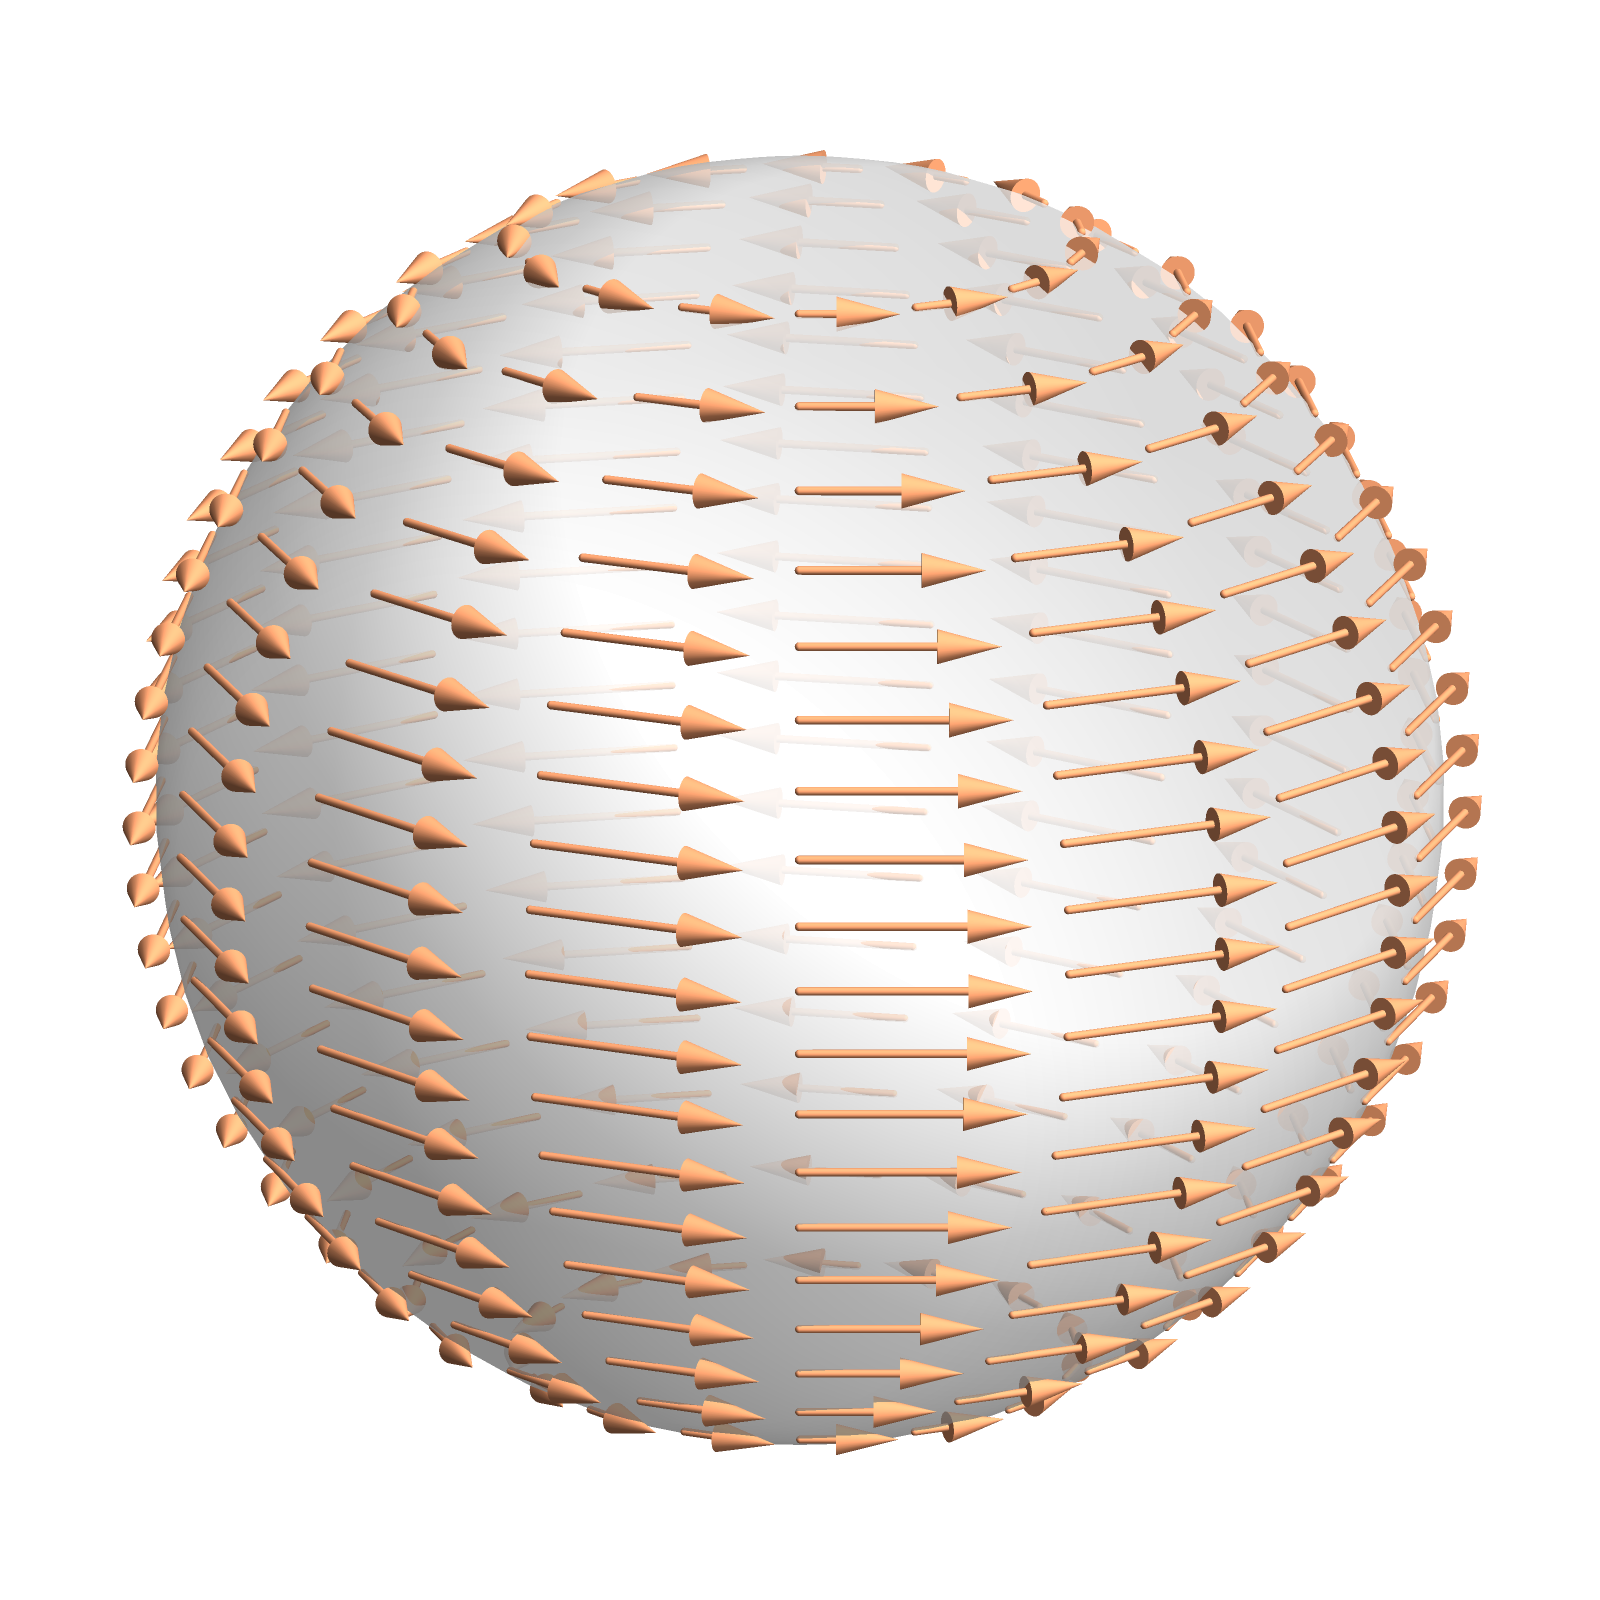
\includegraphics[height=2in]{dtheta} \qquad 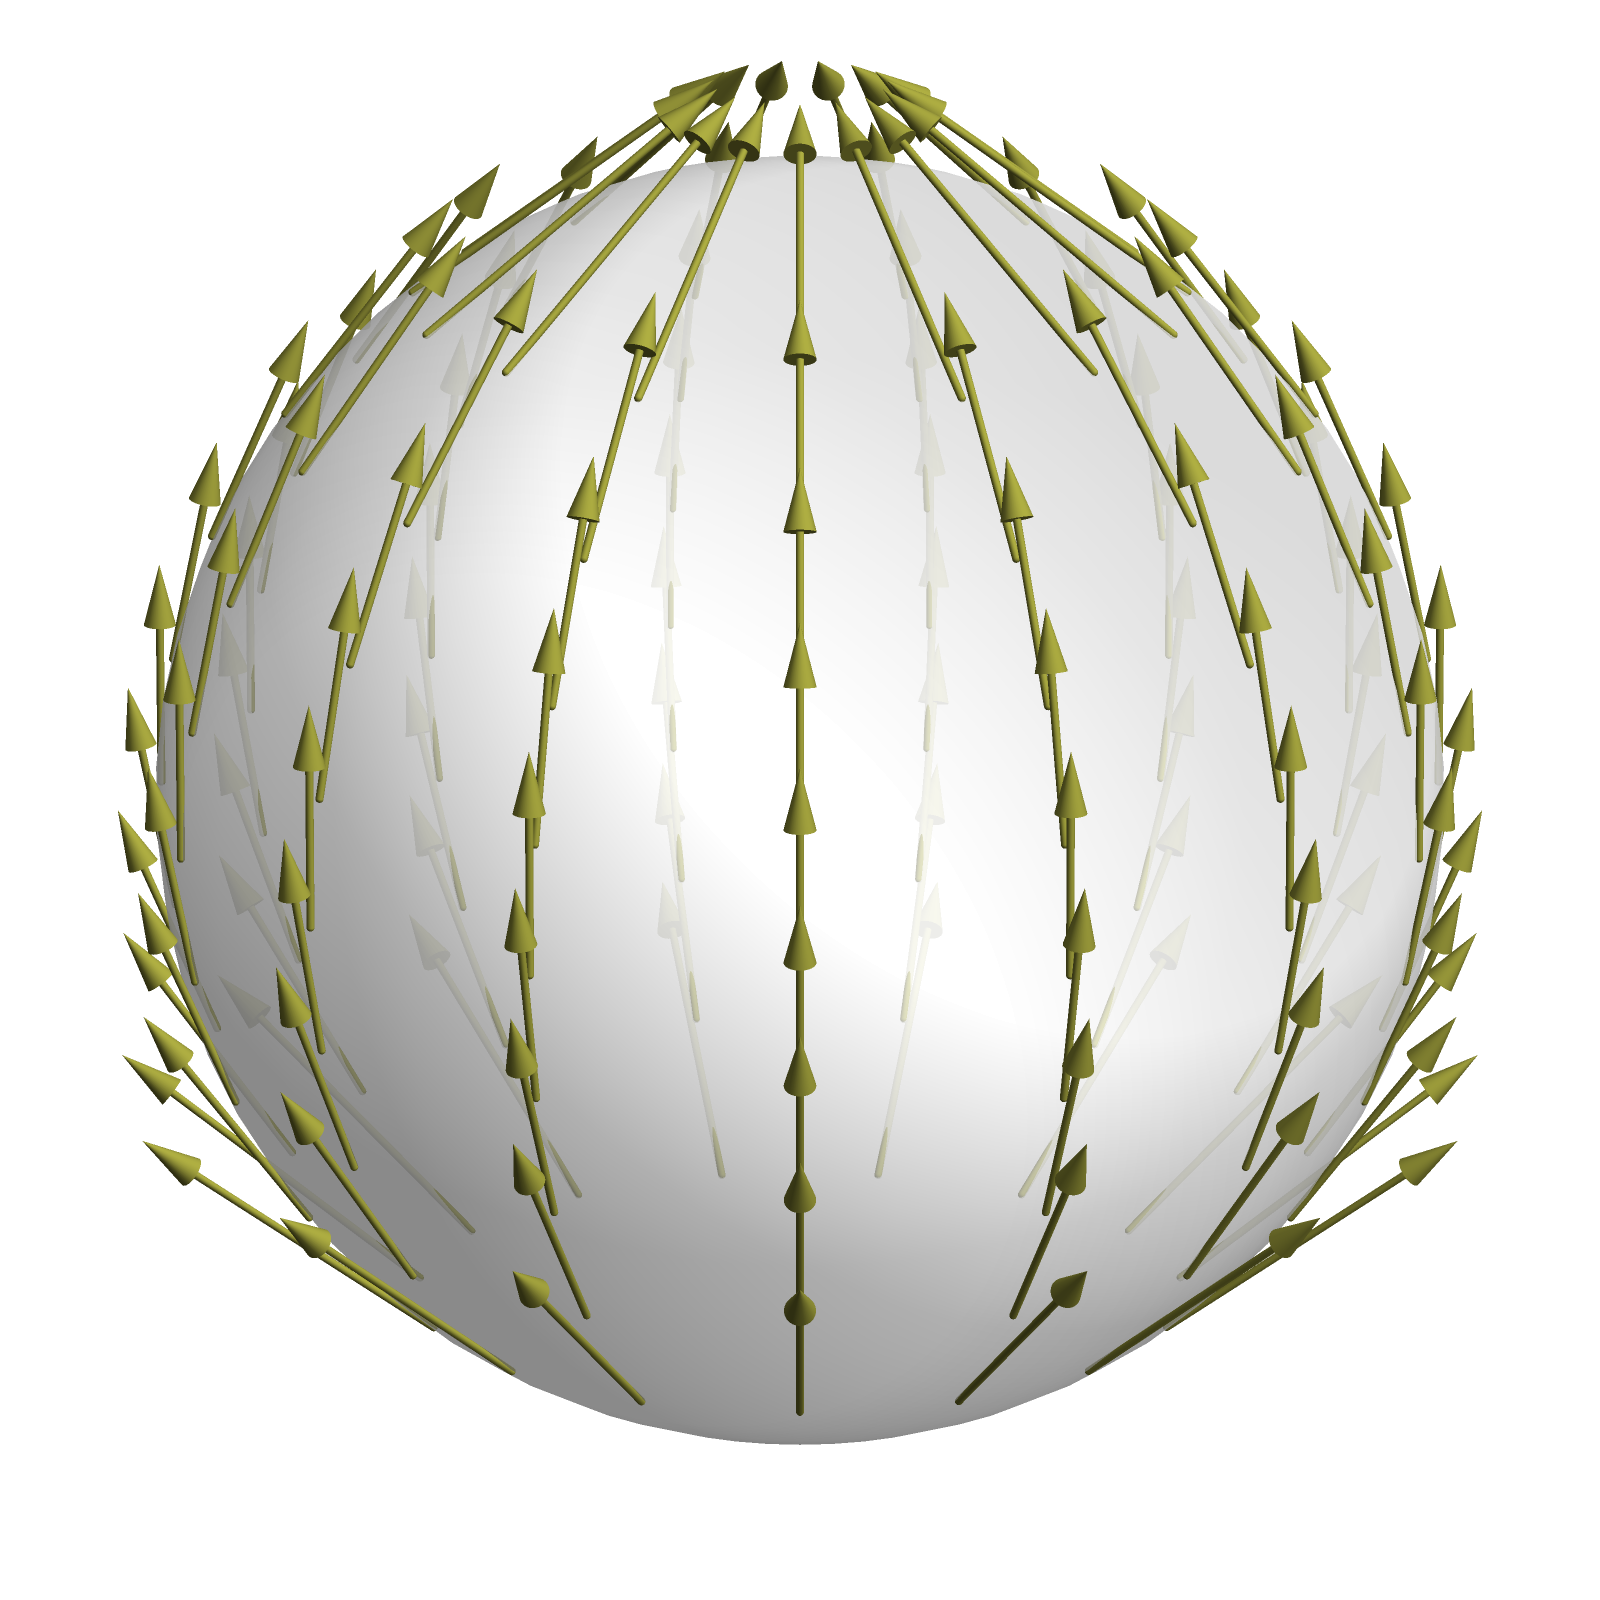
\includegraphics[height=2in]{dz}
		\caption{The vector fields $X = \frac{\partial}{\partial \theta}$ and $Y = \frac{\partial}{\partial z}$ on $S^2$.}
		\alttext{Two computer-generated semi-transparent gray spheres. On the left, a collection of orange arrows or shown on the sphere: the arrows point along circles of latitude: the lengths get shorter as they move away from the equator. On the right, there is a collection of green arrows on the sphere which point towards the north pole. The green arrows get longer as they get further from the equator.}
		\label{fig:dtheta and dz}
	\end{figure}
	
	In other words, we have the local coordinate chart $\phi\from (0,2\pi) \times (-1,1) \to S^2$ given by
	\[
		\phi(\theta,z) = (\sqrt{1-z^2} \cos\theta, \sqrt{1-z^2} \sin \theta, z),
	\]
	and $X$ and $Y$ are the corresponding coordinate fields.
	
	Notice that
	\[
		[X,Y]f = \frac{\partial^2 f}{\partial \theta \partial z} - \frac{\partial^2 f}{\partial z \partial \theta} = 0
	\]
	since mixed partials commute.
	
	More generally, whenever $X = \frac{\partial}{\partial x_i}$ and $Y = \frac{\partial}{\partial x_j}$ are coordinate fields in a neighborhood of a point in a manifold, $[X,Y] = 0$.
	
	In Cartesian coordinates
	\[
		X = \sqrt{1-z^2}\left( - \sin \theta \frac{\partial}{\partial x} + \cos \theta \frac{\partial}{\partial y}\right) = \sqrt{1-z^2}\left( - y \frac{\partial}{\partial x} + x \frac{\partial}{\partial y}\right),
	\]
	and
	\[
		Y = -\frac{z \cos\theta}{\sqrt{1-z^2}}\frac{\partial}{\partial x} - \frac{z \sin\theta}{\sqrt{1-z^2}}\frac{\partial}{\partial y} + \frac{\partial}{\partial z} = -\frac{xz}{1-z^2}\frac{\partial}{\partial x} - \frac{yz}{1-z^2}\frac{\partial}{\partial y} + \frac{\partial}{\partial z}.
	\]
	
	So then some much more unpleasant calculations using \eqref{eq:Lie bracket in local coords} shows you that $[X,Y] = 0$ in these coordinates as well.
\end{example}

Now we look at some examples of Lie algebras not coming from vector fields.

\begin{example}\label{ex:R^3 Lie algebra}
	$\R^3$ forms a Lie algebra with the bracket operation given by the cross product: for $u,v \in \R^3$, define $[u,v] := u \times v$. Then it is straightforward to check that this bracket satisfies \ref{it:Lie bracket anticommutativity}--\ref{it:Lie bracket Jacobi identity} above. Written in terms of cross products, \ref{it:Lie bracket Jacobi identity} says
	\[
		0 = (u \times v) \times w + (v \times w) \times u + (w \times u) \times v = (u \times v) \times w - u \times (v \times w) + v \times (u \times w),
	\]
	or equivalently,
	\[
		(u \times v) \times w = u \times (v \times w) - v \times (u \times w).
	\]
	In particular, this records the failure of associativity of the cross product.
\end{example}

More generally, the Jacobi identity records the failure of associativity of the Lie bracket:
\[
	[[X,Y],Z] = [X,[Y,Z]] - [Y,[X,Z]].
\]

\begin{example}\label{ex:Lie algebra U(d)}
	Recall \Cref{ex:left invariant vector field}, in which we showed that left-invariant vector fields on $\U(d)$ are of the form $X(U) = U \Delta_X$, for $\Delta_X \in T_I\U(d)$, which is the collection of skew-Hermitian $d \times d$ matrices. In particular, $X(I) = \Delta_X$.
	
	As we will see in more detail later (\Cref{prop:matrix group commutator}), it will turn out that the Lie bracket on left-invariant vector fields on a matrix group like $\U(d)$ just corresponds to the matrix commutator operation in the tangent space to the identity. 
	
	In this case, that means that, if $X,Y \in \mathfrak{X}(U(d))$ are left-invariant, then $[X,Y]$ is also left-invariant and, for each $U \in \U(d)$,
	\[
		[X,Y](U) = U(\Delta_X \Delta_Y - \Delta_Y \Delta_X),
	\]
	where the products inside parentheses are just matrix products between the skew-Hermitian matrices $\Delta_X$ and $\Delta_Y$; that is, the term in parentheses is just the usual matrix commutator.
	
	\begin{exercise}
		Check that the commutator of two skew-Hermitian matrices is skew-Hermitian.
	\end{exercise}
	
	This all tells you that the correspondence between left-invariant vector fields and elements of $T_I\U(d)$ turns the Lie bracket of left-invariant vector fields into the matrix commutator in $T_I \U(d)$. These are two different realizations of the same Lie algebra, usually called $\mathfrak{u}(d)$.
\end{example}

\begin{example}\label{ex:so3 Lie algebra}
	If we play the same game with $\SO(d)$, it turns out that the tangent space to the identity consists of $d \times d$ skew-symmetric matrices, and the Lie algebra on left-invariant vector fields on $\SO(d)$ corresponds to the matrix commutator on skew-symmetric matrices; we'll write the collection of skew-symmetric $d \times d$ matrices as $\mathfrak{so}(d)$.
	
	Consider the case $d = 3$. Then we can write elements of $\mathfrak{so}(3)$ as 
	\[
		\Delta = \begin{bmatrix} 0 & -z & y \\ z & 0 & -x \\ -y & x & 0 \end{bmatrix}.
	\]
	(The reason for the funny ordering and sign choices will shortly become apparent.)
	
	Now, $\mathfrak{so}(3)$ is a 3-dimensional vector space, and we have a vector space isomorphism $F\from \R^3 \to \mathfrak{so}(3)$ given by
	\begin{equation}\label{eq:r3 so3 isomorphism}
		F \from (x,y,z) \mapsto \begin{bmatrix} 0 & -z & y \\ z & 0 & -x \\ -y & x & 0 \end{bmatrix}.
	\end{equation}
	
	Let $\Delta_1,\Delta_2 \in \mathfrak{so}(3)$ with 
	\[
		\Delta_i = \begin{bmatrix} 0 & -z_i & y_i \\ z_i & 0 & -x_i \\ -y_i & x_i & 0 \end{bmatrix}.
	\]
	Then
	\[
		[\Delta_1, \Delta_2] = \Delta_1 \Delta_2 - \Delta_2 \Delta_1 = \begin{bmatrix} 0 & x_2 y_1-x_1 y_2 & x_2 z_1-x_1 z_2 \\
 x_1 y_2-x_2 y_1 & 0 & y_2 z_1-y_1 z_2 \\
 x_1 z_2-x_2 z_1 & y_1 z_2-y_2 z_1 & 0 \end{bmatrix}.
	\]
	
	If you stare at this, you might recognize the entries as being the coordinates of the cross product of the corresponding vectors:
	\[
		\begin{bmatrix} x_1 \\ y_1 \\ z_1 \end{bmatrix} \times \begin{bmatrix} x_2 \\ y_2 \\ z_2 \end{bmatrix} = \begin{bmatrix} y_1 z_2-y_2 z_1 \\ x_2 z_1-x_1 z_2 \\ x_1 y_2-x_2 y_1 \end{bmatrix}.
	\]
	In other words, $F(v_1 \times v_2) = [F(v_1), F(v_2)]$, so $F$ is a Lie algebra homomorphism. Since it's also a bijective linear map, it's a Lie algebra isomorphism, so we've just proved that $(\R^3, \times) \cong \mathfrak{so}(3)$ as Lie algebras.
	
	Thus, the Lie bracket on vector fields on manifolds is some sort of vast generalization of the cross product on $\R^3$. In this interpretation, $\R^3 \cong \mathfrak{so}(3)$ is the collection of infinitesimal rotations of 3-space, where $v \in \R^3$ corresponds to an infinitesimal rotation around the axis spanned by $v$, and the correspondence between cross products and commutators reflects the fact that, for very small $\epsilon > 0$ and unit vectors $u$ and $v$, the composition of an $\epsilon$-rotation around $u$ with an $\epsilon$-rotation around $v$ is, to first order, a rotation around $u + v + \frac{\epsilon}{2} u \times v$; see the Baker--Campbell--Hausdorff formula~\cite[Chapter~5]{hallLieGroupsLie2015}.
\end{example}

\begin{exercise}
	Convince yourself that, for $v \in \R^3$ a unit vector and $F$ as defined in \eqref{eq:r3 so3 isomorphism}, $\exp (F(\theta v))$ gives the one-parameter subgroup of rotations by angle $\theta$ around the axis spanned by $v$. (A full proof is kind of annoying to write down, but at least convince yourself this is true when $v$ is a coordinate vector.)
\end{exercise}
% !TEX root = ../dg.tex

\section{Integral Curves and Lie Derivatives}

To motivate the definition of the Lie bracket, I claimed that there was additional algebraic structure on $\mathfrak{X}(M)$ in the form of a binary operation, and then (hopefully!) convinced you that there was really only one sensible way to define such an operation.

But it's probably not at all obvious why one should have guessed that there was a binary operation on vector fields in the first place, and, though I don't actually know the history, my guess is that this was not the original motivation for the Lie bracket.

In some sense the more basic notion is that of the \emph{Lie derivative}, which is a sort of directional derivative of vector fields which, as we will see, actually generalizes to arbitrary tensor fields.

The idea is that, given two vector fields $X$ and $Y$ on a manifold $M$, we might like to define a ``directional derivative of $Y$ in the direction of $X$'' operator, which we will denote $\mathcal{L}_XY$, where the $\mathcal{L}$ is for ``Lie derivative.'' It will turn out that $\mathcal{L}_XY = [X,Y]$, which might be surprising, but if you look back to the local coordinate expression~\eqref{eq:Lie bracket in local coords} for $[X,Y]$, you'll notice it involved differentiating the coefficients of $Y$ with respect to $X$ (and also $X$ with respect to $Y$, but we'll shortly see why there's this symmetry).

It's worth thinking for yourself about how you might go about defining such a derivative operator, so I would encourage you to do so before reading on.

Here's a way of making this ``directional derivative for vector fields'' operation more precise: say we have our vector fields $X$ and $Y$ and we want to compute $\mathcal{L}_XY$ at a point $p \in M$. Presumably the idea is to measure how much $Y$ is changing as we vary $p$ in the direction of $X$. 

In other words, we want to integrate $X$ to get a curve $\alpha: (-\epsilon, \epsilon) \to M$ so that $\alpha(0) = p$ and $\alpha'(t) = X(\alpha(t))$ for all $t \in (-\epsilon, \epsilon)$, then look at something like
\[
	\lim_{t\to 0} \frac{Y(\alpha(t))-Y(\alpha(0))}{t}.
\]
See \Cref{fig:lie-derivative}.

\begin{figure}[htbp]
	\centering
		\includegraphics[height=1.5in]{lie-derivative}
	\caption{An attempt to differentiate $Y$ in the direction of $X$.}
	\label{fig:lie-derivative}
\end{figure}

In other words, we look at the rate of change of $Y$ as we flow in the direction of $X$. Unfortunately, as written the above difference quotient doesn't make sense, but first let's talk about flows and integrating vector fields.

\begin{definition}\label{def:integral curve}
	Let $X \in \mathfrak{X}(M)$. A curve $\alpha\from (a,b) \to M$ is called an \emph{integral curve} (or \emph{trajectory}) for $X$ if $\alpha'(t) = X(\alpha(t))$ for all $t \in (a,b)$. 
\end{definition}

\begin{proposition}\label{prop:local flow}
	Let $X \in \mathfrak{X}(M)$ and let $p \in M$. Then there exists a neighborhood $U$ of $p$, a $\delta > 0$, and a smooth map $\Phi\from (-\delta, \delta) \times U \to M$ so that, for each $q \in U$, the map $t \mapsto \Phi(t,q)$ is the unique smooth curve satisfying the ODE $\frac{\partial \Phi}{\partial t} = X(\Phi(t,q))$ with initial condition $\Phi(0,q) = q$. See \Cref{fig:local-flow}.
\end{proposition}

\begin{figure}[htbp]
	\centering
		\includegraphics[height=1.5in]{local-flow}
	\caption{The local flow generates an integral curve through each point.}
	\label{fig:local-flow}
\end{figure}

\begin{proof}
	Since $M$ is locally diffeomorphic to $\R^n$ (via the coordinate charts), this follows from the fundamental theorem on existence and uniqueness of solutions to ODEs in $\R^n$.
\end{proof}

We often use the notation $\Phi_t(q):=\Phi(t,q)$ and call $\Phi_t$ the \emph{local flow} of $X$.

\begin{example} 
	Let $M = S^2$ and consider the vector field $X(x,y,z) = zx \frac{\partial}{\partial x} + zy \frac{\partial}{\partial y} +\left(z^2-1\right) \frac{\partial}{\partial z}$ (of course, this is written in extrinsic $\R^3$ coordinates rather than intrinsic coordinates). See \Cref{fig:flowfield}.
	
	\begin{figure}[htbp]
		\centering
			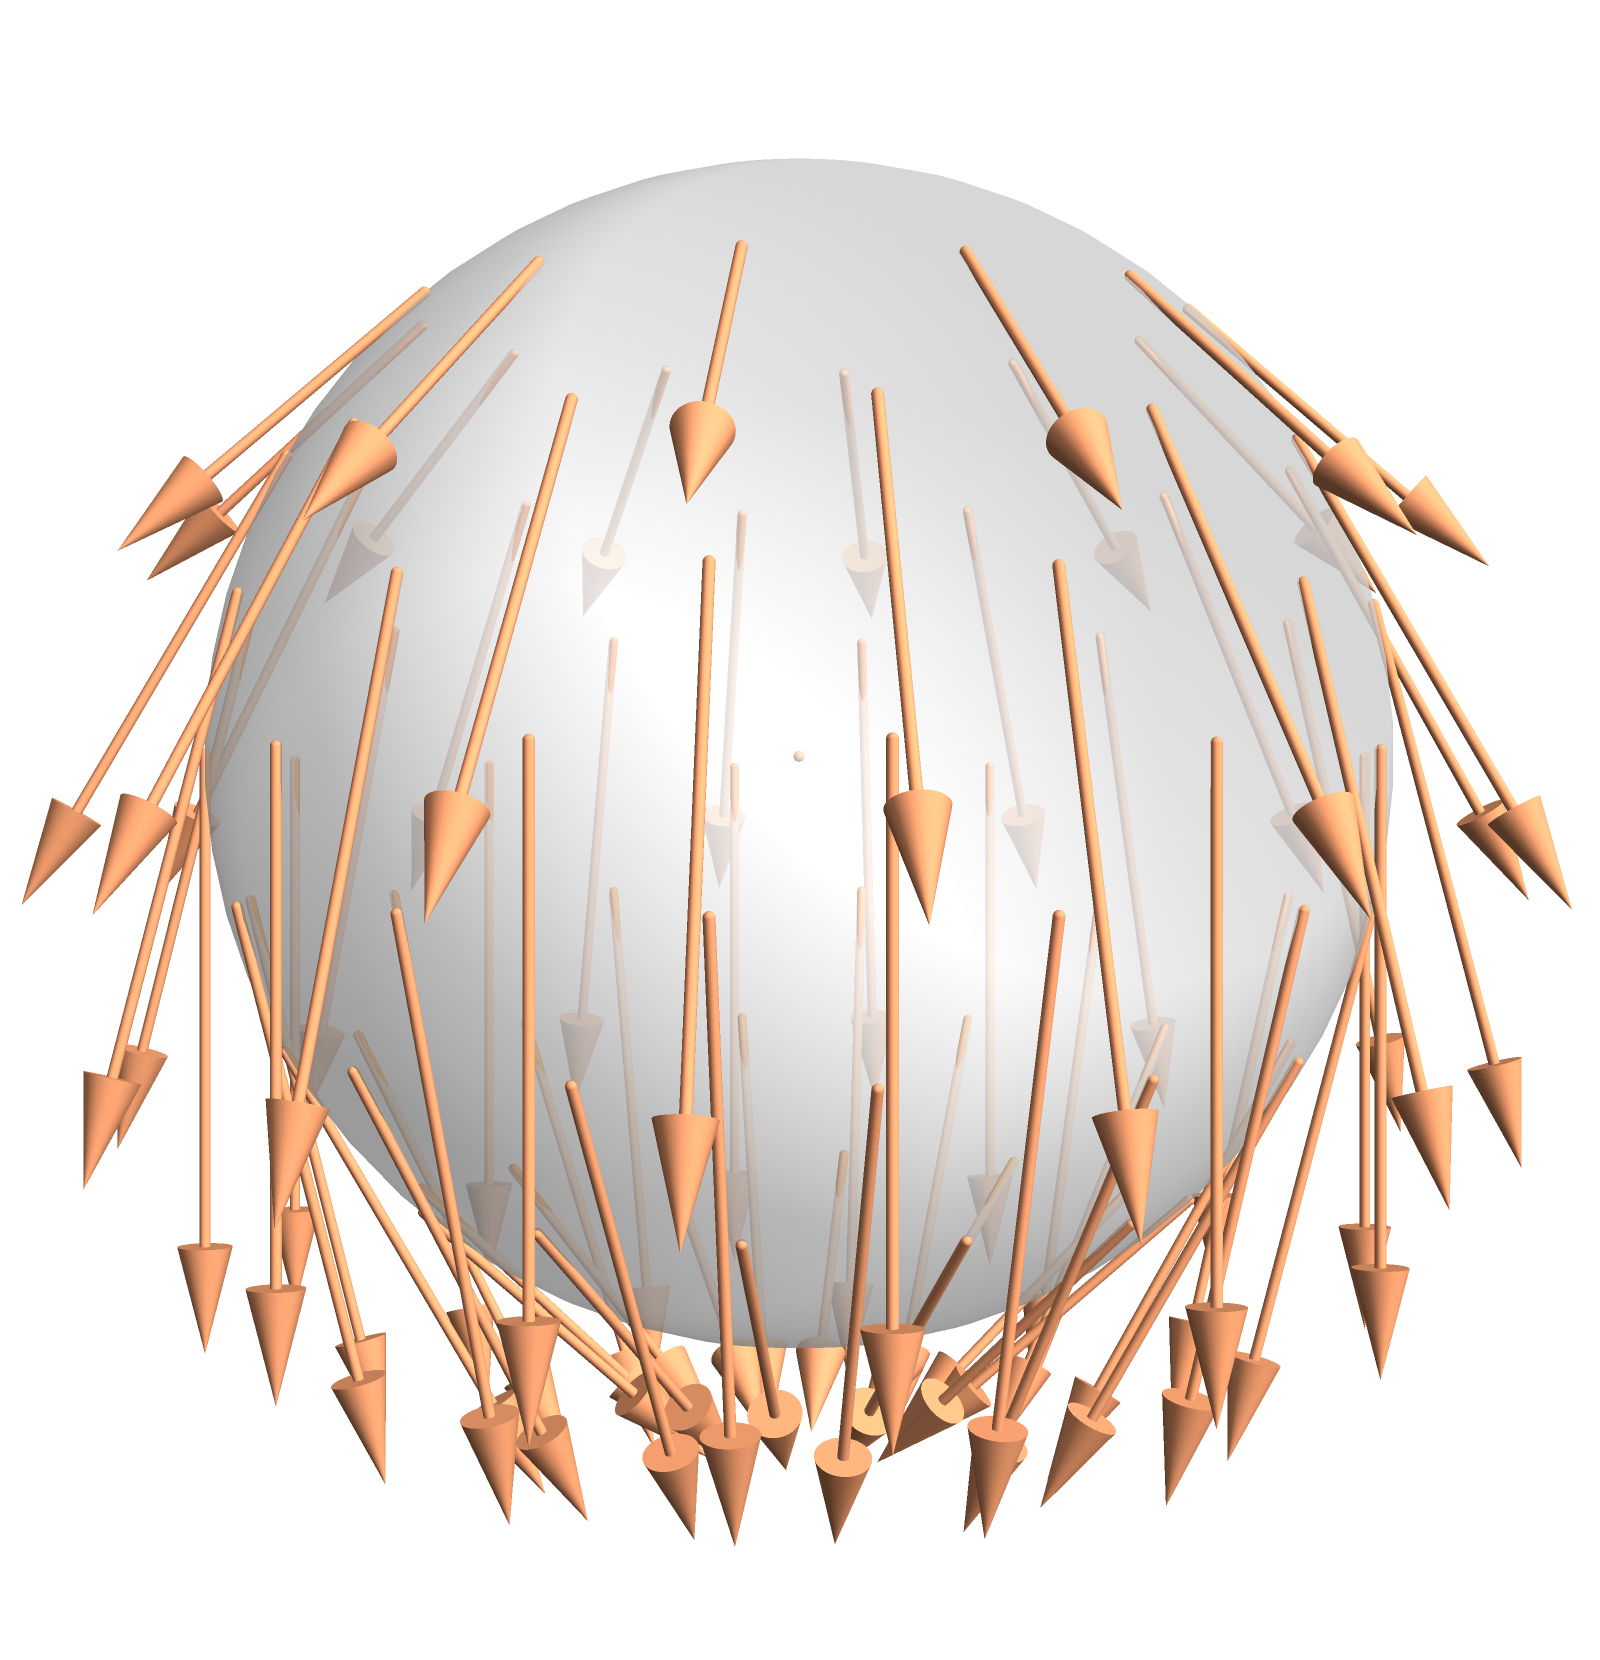
\includegraphics[height=2in]{flowfield}
		\caption{The vector field $X(x,y,z) = zx \frac{\partial}{\partial x} + zy \frac{\partial}{\partial y} +\left(z^2-1\right) \frac{\partial}{\partial z}$ on the sphere.}
		\label{fig:flowfield}
	\end{figure}
	
	In fact, you can check that this is just $(d\phi_N)Y$, where $Y$ is the vector field on $\R^2$ given by $Y(u,v) = -u \frac{\partial}{\partial u} - v \frac{\partial }{\partial v}$.
	
	Visually, the local flow pushes the mass of the sphere down towards the south pole. We can integrate the flow explicitly in \emph{Mathematica} to get
	\[
		\Phi_t(x,y,z) = \frac{1}{1+2e^{2t} + \left(1-e^{2t}\right)z}\left(2e^t x, 2e^t y, 1-e^{2t} + \left(1+e^{2t}\right)z\right).
	\]
	See \Cref{fig:conformalflow}.
	
	\begin{figure}[htbp]
		\centering
			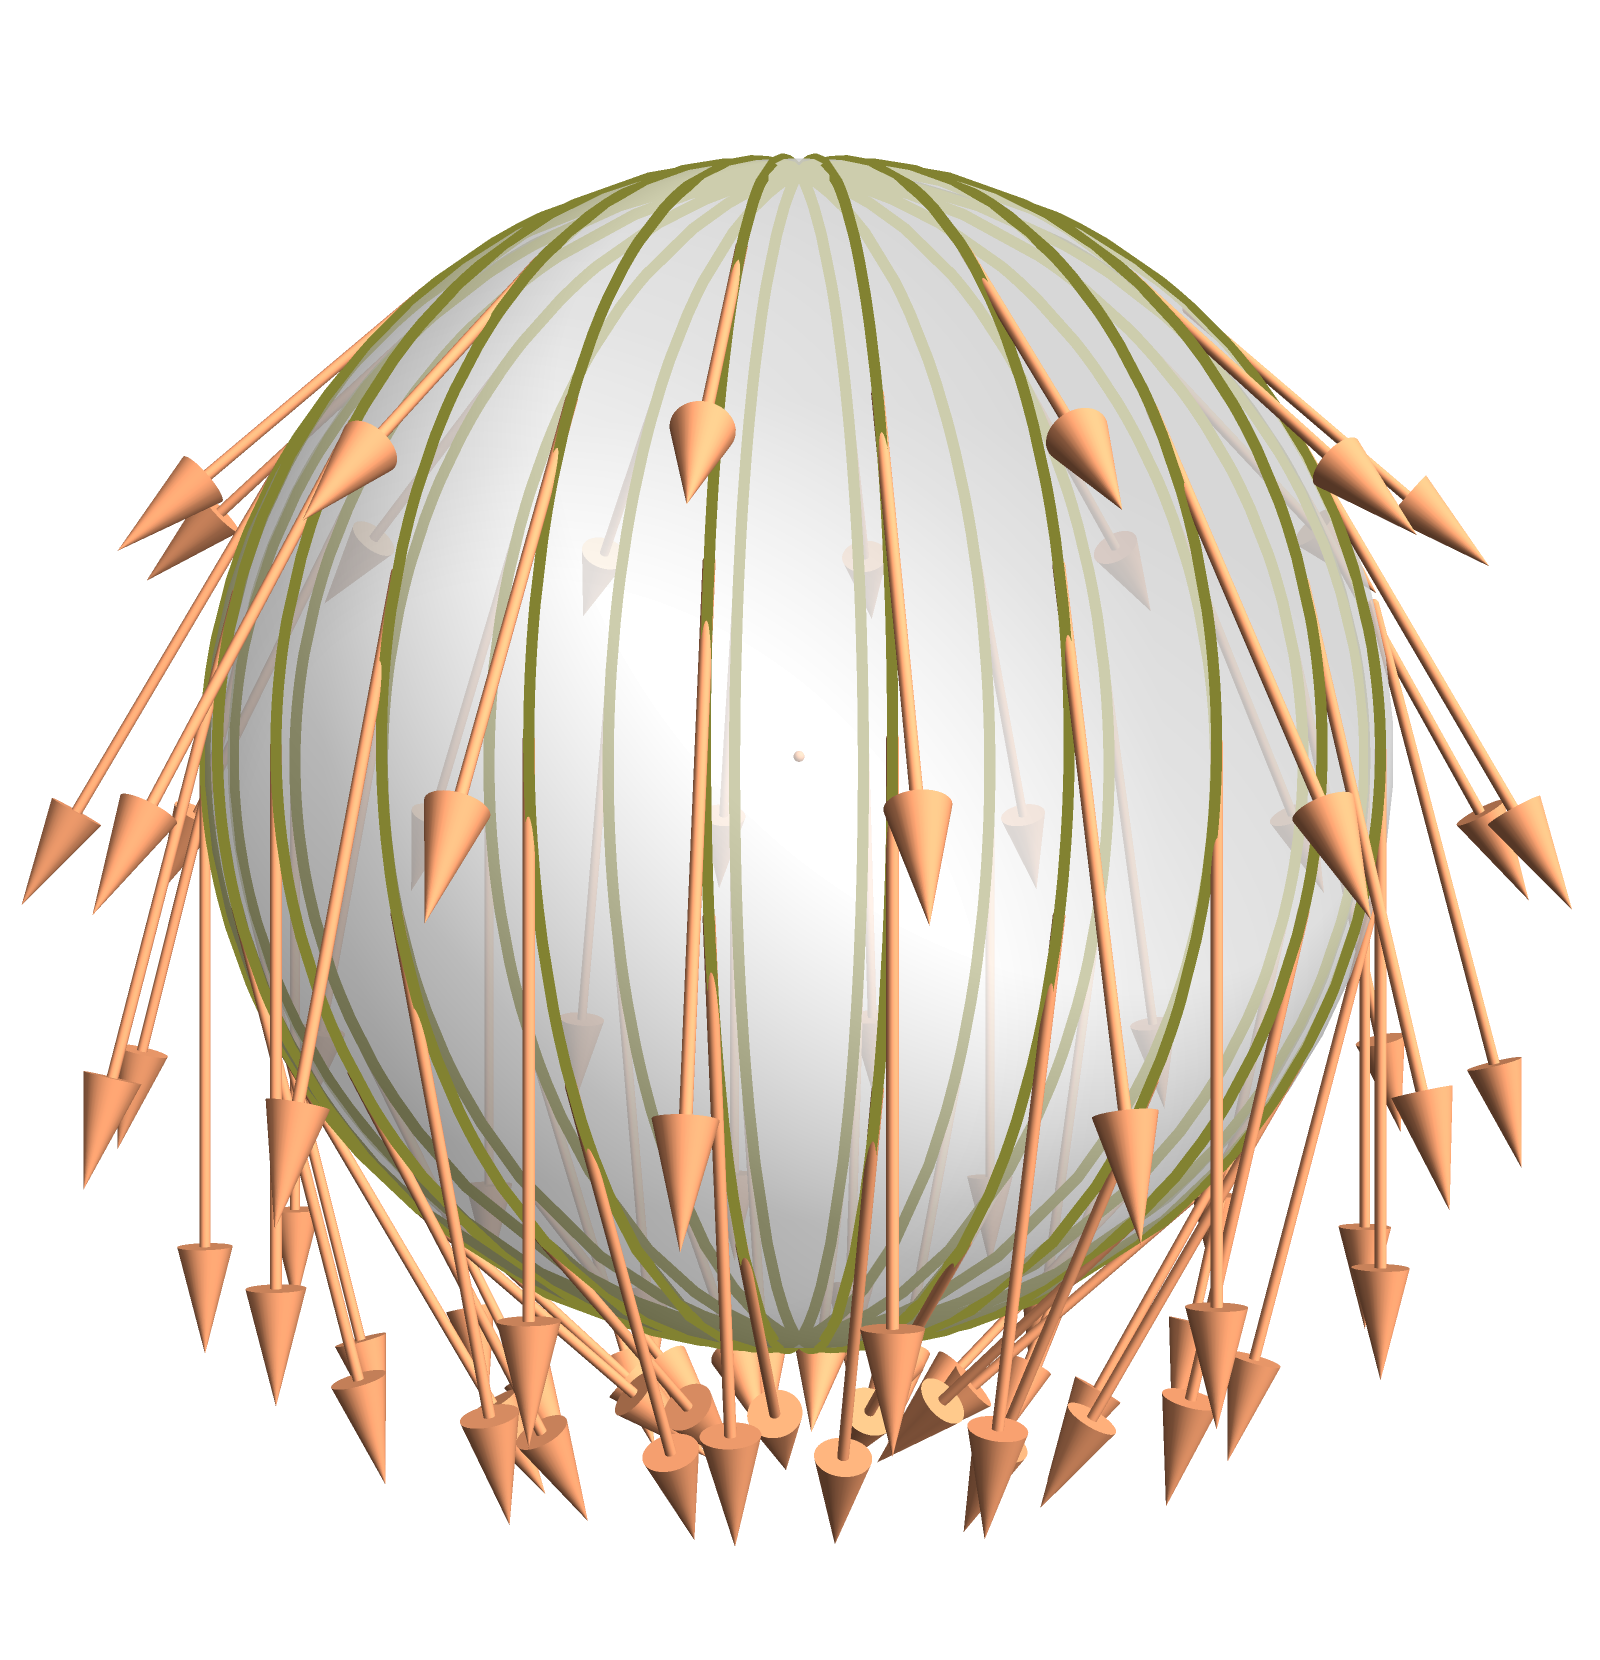
\includegraphics[height=2in]{conformalflow}
		\caption{The local flow of $X$.}
		\label{fig:conformalflow}
	\end{figure}
	
	This is an example of a \emph{complete vector field} since the local flow exists for all time at all points. If we had removed the Antarctic Circle from the sphere, this vector field would be incomplete (since the flow ceases to exist once you go over the edge).
\end{example}

With local flows in our toolkit we would then like to define the Lie derivative as something like
\[
	(\mathcal{L}_XY)(p) = \lim_{t \to 0} \frac{Y(\Phi_t(p)) - Y(p)}{t}.
\]
But if you think about it, the numerator in the difference quotient \emph{makes no sense!} After all, $Y(\Phi_t(p)) \in T_{\Phi_t(p)}M$ and $Y(p) \in T_pM$ live in completely different vector spaces. There's no sense in which we can subtract these two vectors.

So we need some way to get the tangent vectors determined by $Y$ at different points to be in the same tangent space.

Thus far, the only machines we have for moving tangent vectors between different tangent spaces are differentials of smooth maps. The only smooth map we have at our disposal is $\Phi_t$, so somehow that must come into play. One possibility is
\[
	\lim_{t \to 0} \frac{Y(\Phi_t(p)) - (d \Phi_t)_p Y(p)}{t}
\]
since both $Y(\Phi_t(p))$ and $(d \Phi_t)_pY(p)$ live in $T_{\Phi_t(p)}M$. The problem with this is that, as $t$ changes, $T_{\Phi_t(p)}M$ is also changing, so we're taking limits of vectors in different tangent spaces. Now, all these tangent vectors still live in $TM$, so this is in fact doable, but it would be better if all the vectors in the limit actually lived in the tangent space, ideally $T_pM$. 

We are finally ready to define the Lie derivative:

\begin{definition}\label{def:Lie derivative}
	Suppose $M$ is a manifold, $X,Y \in \mathfrak{X}(M)$, and $p \in M$. Then the \emph{Lie derivative} of $Y$ with respect to $X$ at $p$ is
	\[
		(\mathcal{L}_XY)(p) := \lim_{t \to 0} \frac{(d \Phi_{-t})_{\Phi_t(p)}Y(\Phi_t(p)) - Y(p)}{t},
	\]
	where $\Phi_t$ is the local flow for $X$.
\end{definition}

This is a lot of obnoxious notation, but let's try to unpack it. First of all, notice that $\Phi_{-t}(\Phi_t(p)) = p$, since we're just flowing forward in time by $t$ and then backwards for the same time. So
\[
	(d\Phi_{-t})_{\Phi_t(p)}\from T_{\Phi_t(p)}M \to T_p M.
\]
Hence, plugging in $Y(\Phi_t(p))$ gives $(d\Phi_{-t})_{\Phi_t(p)}Y(\Phi_t(p)) \in T_pM$, and the difference quotient and the limit make sense as happening entirely in $T_pM$. A (somewhat messy) picture is shown in \Cref{fig:lie-derivative2}.

\begin{figure}[htbp]
	\centering
		\includegraphics[height=1.5in]{lie-derivative-2}
	\caption{The pieces in the definition of $\mathcal{L}_XY$.}
	\label{fig:lie-derivative2}
\end{figure}

In looking at \Cref{fig:lie-derivative2}, recall that the point was that we wanted to see how $Y$ varied as we moved in the direction of $X$. So at a point $p \in M$, we follow the local flow of $X$ for a small time $t$. $Y$ determines a tangent vector at the resulting point $\Phi_t(p)$. Now we push this vector $Y(\Phi_t(p))$ to $T_pM$ by the negative local flow of $X$ and compare to $Y(p)$.

You can imagine that if $Y$ had a constant magnitude and made a constant angle with $X$, then pushing $Y$ forward by the negative local flow (which is exactly $(d\Phi_{-t})_{\Phi_t(p)}Y(\Phi_t(p))$) would just give you the same vector you started with, namely $Y(p)$. But this makes sense: if $Y$ has a constant magnitude and makes a constant angle with $X$, then it's not changing at all with respect to $X$, and this derivative should really be 0.\footnote{You should take this paragraph figuratively and not literally: we don't have any notion of magnitude or angle for tangent vectors, because we don't yet have inner products on the tangent spaces. That will come when we start talking about Riemannian metrics!}

The slightly amazing fact is that the Lie derivative and the Lie bracket are the same:

\begin{proposition}\label{prop:Lie bracket = Lie derivative}
	Let $X,Y \in \mathfrak{X}(M)$ and choose $p \in M$. Then
	\[
		[X,Y](p) = (\mathcal{L}_XY)(p).
	\]
\end{proposition}

Notice, in particular, that this shows that the Lie derivative is antisymmetric:
\[
	\mathcal{L}_YX = [Y,X] = -[X,Y] = - \mathcal{L}_XY
\]
by the antisymmetry of the Lie bracket, which you might not have guessed from the definition of the Lie derivative.

\begin{proof}[Proof of \Cref{prop:Lie bracket = Lie derivative}]
	Both expressions are tangent vectors at $p$, so formally they're differential operators evaluated on functions that are differentiable in a neighborhood of $p$. So we'll choose a test function $f$ which is differentiable in a neighborhood of $p$, and the goal is to show that
	\[
		\lim_{t \to 0} \frac{(d\Phi_{-t})_{\Phi_t(p)}Y(\Phi_t(p))-Y(p)}{t}(f)(p) = ((XY-YX)f)(p).
	\]
	Let's focus on the first term in the numerator, $\left((d\Phi_{-t})_{\Phi_t(p)}Y)f\right)(p)$:
	\[
		\left((d\Phi_{-t})_{\Phi_t(p)}Y)f\right)(p) = (df_p)(((d\Phi_{-t})_{\Phi_t(p)}Y)(p)) = (d(f \circ \Phi_{-t})_{\Phi_t(p)}Y(\Phi_t(p))) = (Y(f\circ \Phi_{-t}))(\Phi_t(p)),
	\]
	where we used \Cref{lem:vector fields and differentials} for the first and last equalities\footnote{Note: I added this lemma after the initial draft, so it was not there when you previously read that section.} and the chain rule for the middle equality. Therefore,
	\[
		(\mathcal{L}_XY)(p) = \lim_{t \to 0} \frac{(Y(f \circ \Phi_{-t}))(\Phi_t(p))-(Yf)(p)}{t}.
	\]
	
	If we could turn this into something like 
	\begin{equation}\label{eq:XYf}
		\lim_{t \to 0} \frac{(Yf)(\Phi_t(p)) - (Yf)(p)}{t} = \left. \frac{d((Yf)\circ \Phi_t)}{dt} \right|_{t = 0} = (X(Yf))(p),
	\end{equation}
	we'd be in business.
	
	In fact, if we could write $f(\Phi_{-t}(q)) = f(q) + t g(t,q)$ for some function $g$, then we could get a term like~\eqref{eq:XYf} to appear because then we'd have
	\begin{align*}
		\lim_{t \to 0} \frac{(Y(f \circ \Phi_{-t}))(\Phi_t(p))-(Yf)(p)}{t} & = \lim_{t \to 0} \frac{(Y(f +t g(t, \cdot)))(\Phi_t(p))-(Yf)(p)}{t} \\
		& = \lim_{t \to 0} \frac{(Yf)(\Phi_t(p)) + (Y(t g(t, \cdot)))(\Phi_t(p))-(Yf)(p)}{t} \\
		& = \lim_{t \to 0} \frac{(Yf)(\Phi_t(p)) + t(Y( g(t, \cdot)))(\Phi_t(p))-(Yf)(p)}{t} \\
		& = \lim_{t \to 0} \frac{(Yf)(\Phi_t(p)) -(Yf)(p)}{t} + Y(g(0,\Phi_0(p)) \\
		& = (X(Yf))(p) + Y(g(0,p)).
	\end{align*}
	This will then equal $((XY-YX)f)(p)$ if we can find such a $g$ so that the expression $Y(g(0,p))$ is equal to $(Y(Xf))(p)$.
	
	But this is easy: rearranging $f(\Phi_{-t}(q)) = f(q) + tg(t,q)$ yields
	\[
		g(t,q) = \frac{f(\Phi_{-t}(q))-f(q)}{t},
	\]
	at least for $t \neq 0$. We can extend the definition to $t=0$ by taking the limit:
	\[
		g(0,q) := \lim_{t \to 0} \frac{f(\Phi_{-t}(q)) - f(q)}{t} = (Xf)(q),
	\]
	which is exactly what we need, since then $Y(g(0,p)) = (Y(Xf))(p)$.
\end{proof}


% !TEX root = ../dg.tex

\section{Extended Example on $S^3$}
\label{sec:S^3 example}

Let $S^3$ be the unit sphere in $\R^4 \cong \C^2 \cong \quat$, where 
\[
	\quat = \{ a + bi + cj + dk : a,b,c,d\in \R\}
\]
is the division ring of quaternions. We have the defining conditions
\[
	i^2=j^2=k^2 = -1, \qquad ijk = -1,
\]
which for example imply that 
\[
	-ij = ijk^2 = (ijk)k = -k \Rightarrow ij=k
\]
and
\[
	-ji = ji(ijk) = ji^2jk = -j^2k = k \Rightarrow ji = -k,
\]
so $\quat$ is noncommutative. $\quat$ also has a conjugation operation defined by 
\[
	\overline{a+bi+cj+dk} = a-bi-cj-dk
\]
and an inner product given by,
\[
	\langle p,q \rangle = \operatorname{Re}(p\overline{q}).
\]
When $p = a+bi+cj+dk$ and $q = t + xi + yj + zk$, we see that
\[
	\langle p , q \rangle = \operatorname{Re}(p\overline{q}) = \operatorname{Re}((a+bi+cj+dk)(t-xi-yj-zk)) = at+bx+cy+dz,
\]
so this agrees with the usual dot product on $\R^4$. Moreover, the induced norm
\[
	\|p\|^2 = \langle p, p\rangle = \operatorname{Re}(p \overline{p}) = \operatorname{Re}((a+bi+cj+dk) (a-bi-cj_dk)) = a^2 + b^2 + c^2 + d^2
\]
is the standard one.

Thought of as the unit quaternions $\{q \in \quat : \|q\| = 1\}$, it becomes clear that $S^3$ is a group: if $p = a+bi+cj+dk , q = t + xi + yj + zk \in \quat$ are both unit quaternions, meaning that
\[
	a^2 + b^2 + c^2 + d^2 = p \overline{p} = \|p\|^2 = 1 = \|q\|^2 = q \overline{q} = t^2 + x^2 + y^2 + z^2,
\]
then their product is also a unit quaternion:
\[
	\|pq\| = (pq)(\overline{pq}) = p q \overline{q}\, \overline{p} = p 1 \overline{p} = p \overline{p} = 1.
\]

To give some other terminology, $S^3$ is the \emph{symplectic group} $\Sp(1)$; that is, the quaternionic analog of the unitary group for $\quat^1$. (We will eventually see that this group is also isomorphic to $\SU(2)$ and $\Spin(3)$).

Geometrically, it is clear that, for any $p \in S^3$, the tangent space $T_pS^3$ can be thought of as the quaternions which are orthogonal to $p$. So for example the tangent space to the identity $1 \in S^3$ is
\[
	T_1 S^3 = \{xi + yj + zk : x,y,z \in \R^3\},
\]
the purely imaginary quaternions. Using the same idea as in \Cref{ex:left invariant vector field}, we can push any tangent vector at the identity around to get a left-invariant vector field on all of $S^3$. In particular, we get three mutually perpendicular vector fields $X,Y,Z \in \mathfrak{X}(S^3)$ given by
\[
	X(p) = pi, \quad Y(p) = pj, \quad Z(p) = pk
\]
for all $p \in S^3$. (Strictly speaking, $X(p) = (d L_p)_1 i$, where $L_p$ is left-multiplication by $p$, and $i$ is intepreted as an element of $T_1S^3$ [and similarly for $Y$ and $Z$], but $L_p$ being linear implies that $(dL_p)_1 i = pi$.)

To check that, say, $X(p)$ is really a tangent vector at $p$, notice that
\[
	\langle p, X(p)\rangle = \langle p, pi\rangle = \langle a + bi + cj + dk, -b + ai+dj-ck\rangle = -ab+ab-cd+cd = 0,
\]
so $X(p) \bot p$ and hence $X(p) \in T_pS^3$. Similar calculations show that $Y(p),Z(p) \in T_p S^3$.

Moreover $X$, $Y$, and $Z$ are mutually perpendicular everywhere: for example
\[
	\langle X(p) , Y(p) \rangle = \langle pi, pj\rangle = \langle -b+ai+dj-ck, -c-di+aj+bk\rangle = bc-ad+ad-bc = 0.
\]
(A better argument: multiplication by a unit quaternion is an isometry of $\quat = \R^4$, so orthogonality of $X(1) = i$ and $Y(1) = j$ carries over to $T_pS^3$.)

Now, the corresponding local flows are
\[
	\xi_t(p) = p(\cos t + i \sin t), \quad \psi_t(p) = p(\cos t + j \sin t), \quad \zeta_t(p) = p(\cos t + k \sin t),
\]
as we can see by differentiating; for example,
\[
	\left. \frac{d}{dt}\right|_{t=0} \xi_t(p) = \left. \frac{d}{dt}\right|_{t=0}p (\cos t + i \sin t) = -p \sin(0) + p i \cos(0) = pi = X(p).
\]

Now we compute some Lie brackets. For example,
\begin{align*}
	[X,Y](p) = (\mathcal{L}_XY)(p) & = \lim_{t \to 0} \frac{(d\xi_{-t})_{\xi_t(p)}Y(\xi_t(p))-Y(p)}{t} \\
	& = \left. \frac{d}{dt}\right|_{t=0} (d\xi_{-t})(Y(\xi_t(p))) \\
	& = \left. \frac{d}{dt}\right|_{t=0} (d\xi_{-t})(\xi_t(p)j) \\
	& = \left. \frac{d}{dt}\right|_{t=0} (d\xi_{-t})(p(\cos t + i \sin t)j) \\
	& = \left. \frac{d}{dt}\right|_{t=0} (d\xi_{-t})(p(j\cos t + k \sin t)).
\end{align*}

The differential $(d\xi_{-t})_{\xi_t(p)}\from T_{\xi_t(p)}S^3 \to T_p S^3$, but we can interpret both of these as subspaces of the ambient space $\R^4$, so the differential can be represented by a $4 \times 4$ matrix, namely
\[
	(d \xi_{-t})_{\xi_t(p)} = \begin{bmatrix} \cos t& \sin t & 0 & 0 \\ -\sin t & \cos t & 0 & 0 \\ 0 & 0 & \cos t & -\sin t \\ 0 & 0 & \sin t & \cos t \end{bmatrix},
\]
so
\[
	(d\xi_{-t})(p(j\cos t + k \sin t)) = \begin{bmatrix} \cos t& \sin t & 0 & 0 \\ -\sin t & \cos t & 0 & 0 \\ 0 & 0 & \cos t & -\sin t \\ 0 & 0 & \sin t & \cos t \end{bmatrix} \begin{bmatrix} -c \cos t - d \sin t \\ c \sin t - d \cos t \\ a \cos t - b \sin t \\ a \sin t + b \cos t \end{bmatrix} = \begin{bmatrix} -c \cos 2t - d \sin 2t \\ c \sin 2t - d \cos 2t \\ a \cos 2t - b \sin 2t \\ a \sin 2t + b \cos 2t \end{bmatrix}.
\]

Putting this all together, then
\[
	[X,Y](p) =\left. \frac{d}{dt}\right|_{t=0} (d\xi_{-t})(p(j\cos t + k \sin t)) = \begin{bmatrix} -2d \\ 2c \\ -2b \\ 2a \end{bmatrix} = 2pk = 2Z(p).
\]
In other words, $[X,Y] = 2Z$ and, by similar arguments, $[Y,Z] = 2X$ and $[Z,X] = 2Y$.

In our language from \Cref{ex:left invariant vector field}, $X$, $Y$, and $Z$ are left-invariant vector fields on the Lie group $S^3$, and so you should expect that the Lie bracket on left-invariant vector fields on $S^3$ corresponds to a Lie algebra structure on $T_1 S^3$, which is a 3-dimensional vector space. We'll call this 3-dimensional Lie algebra $\mathfrak{sp}(1)$ since $S^3 = \Sp(1)$. 

Thinking of $S^3$ and $\mathfrak{sp}(1)$ as living in the space of $1 \times 1$ quaternionic matrices (that is, inside $\quat$), we might expect that the matrix commutator on $\mathfrak{sp}(1) = \{xi + yj + zk\}$ should correspond to the above Lie bracket. Indeed, the commutator of the $1 \times 1$ matrices $i$ and $j$ is
\[
	ij - ji  = k - (-k) = 2k,
\]
which agrees with the above calculation that $[X,Y] = 2Z$.


Since the only Lie algebra structure we've seen on a 3-dimensional vector space is that of $(\R^3,\times)$, or equivalently $(\mathfrak{so}(3),[\cdot,\cdot])$, you might guess that $\mathfrak{sp}(1)$ is just another iteration of the same Lie algebra.

Indeed, if $e_1, e_2 , e_3$ is the standard basis for $\R^3$ and we define $F\from \R^3 \to \mathfrak{sp}(1)$ by
\[
	F(e_1) = \frac{1}{2} X, \qquad F(e_2) = \frac{1}{2} Y, \qquad F(e_3) = \frac{1}{2} Z,
\]
then we see that, e.g.,
\[
	 F(e_1 \times e_2) = F(e_3) =  \frac{1}{2}Z = \frac{1}{4}[X,Y] = \left[ \frac{1}{2}X, \frac{1}{2}Y\right] = [F(e_1),F(e_2)],
\] 
and more generally it's easy to check that $F(u\times v) = [F(u),F(v)]$ for any $u,v \in \R^3$, so $F$ is an isomorphism of Lie algebras. 

This also implies that $\mathfrak{so}(3)$ and $\mathfrak{sp}(1)$ are isomorphic Lie algebras, even though the Lie groups $\SO(3)$ and $S^3$ are not even homotopy equivalent (for example, $\pi_1(\SO(3))\cong \Z/2\Z$ and $\pi_1(S^3) = \{1\}$), which is going to imply that they cannot be isomorphic as Lie groups.\footnote{That said, $\SO(3) \cong \RP^3$ has $S^3$ as its universal cover; indeed, this is really what the isomorphism of Lie algebras implies.}

\chapter{Differential Forms}

% !TEX root = ../dg.tex

\section{Integration, Forms, and an Informal Definition}
\label{sec:informal def of forms}

% Add some stuff about how we've defined various notions of derivative, so it's time to start thinking about integrals.

Now that we've defined vector fields and explored some special features (like the Lie bracket), the next objects to turn our attention to are \emph{differential forms}. Differential forms turn out to be the right tool with which to define integration on manifolds, and they also turn out to encode the cohomology ring of a manifold, which means they have both a natural binary operation (corresponding to the cup product in cohomology) and a natural derivative operation (corresponding to the coboundary map).

To try to build up some intuition for differential forms, think back to vector calculus and computing integrals of the form
\begin{equation}\label{eq:multivariable calculus integral}
	\int_A f\, dx_1 \dots dx_n,
\end{equation}
where $A \subseteq \R^n$ is an open set (or maybe the closure of an open set), and $f: A \to \R$ is a (sufficiently nice) function.\footnote{For our purposes we'll just be dealing with the Riemann integral, but one can also generalize the Lebesgue integral to manifolds.} If you stare at \eqref{eq:multivariable calculus integral}, and in particular at the expression $f\, dx_1 \dots dx_n$ being integrated, what exactly is this thing?

To get a handle on what it is, it's helpful to see how it transforms. If $B \subseteq \R^n$ is open and $g: B \to A$ is a diffeomorphism,\footnote{In calculus terms, this is a change of variables; e.g., a transition from Cartesian to spherical coordinates.} then
\[
	\int_A f\, dx_1 \dots dx_n = \int_B (f \circ g) \,|\!\det Jg|\, dy_1 \dots dy_n,
\]
where I'm using $y_1, \dots , y_n$ to indicate the coordinates on $B$ and $Jg$ is the Jacobian matrix of $g$. So now whatever kind of object $f\, dx_1 \dots dx_n$ is, it's the same type of object as $(f \circ g) \,|\!\det Jg|\, dy_1 \dots dy_n$, and this describes how it transforms under diffeomorphisms.

Now, examining $(f \circ g)\, |\!\det Jg|\, dy_1 \dots dy_n$, it's clear that this is a more complicated object than just a function. In particular, the presence of the determinant tells you that this is some sort of \emph{alternating}, \emph{multilinear} object. Recall the definitions:

\begin{definition}\label{def:multilinear}
	Let $V_1, \dots , V_k, W$ be $R$-modules. A map
	\[
		f \from V_1 \times \dots \times V_k \to W
	\]
	is \emph{multilinear} if it is linear in each factor. That is, for any $j \in \{1, \dots , k\}$, if $v_i \in V_i$ for each $i=1, \dots , k$, $u_j \in V_j$, and $c \in \R$, then
	\[
		f(v_1, \dots , u_j + c v_j , \dots , v_k) = f(v_1, \dots , u_j, \dots , v_k) + c f(v_1, \dots , v_j, \dots , v_k).
	\]
\end{definition}

\begin{definition}\label{def:alternating}
	Let $V$ and $W$ be $R$-modules. A multilinear map $f\from V^k \to W$ is \emph{alternating} if, for any $i \neq j$, $v_i = v_j$ implies that $f(v_1, \dots , v_k) = 0$.
\end{definition}

Thinking of the determinant map as a function $\det\from V^n \to \R$ where $(v_1, \dots , v_n) \in V^n$ are interpreted as the columns of a matrix whose determinant is then computed, $\det$ is multilinear and alternating. Indeed, these two properties uniquely characterize the determinant up to scale:

\begin{theorem}\label{thm:determinant}
	Suppose $V$ is an $n$-dimensional vector space. Up to scaling by a constant factor, $\det$ is the unique alternating, multilinear map $V^n \to \R$. 
\end{theorem}

The point of all of this is that the things we actually integrate in multivariable calculus are alternating, multilinear gadgets. Informally, this is how we should think about differential forms on manifolds:

\begin{definition}[Informal Definition]\label{def:informal differential form}
	A smooth \emph{differential $k$-form} on a manifold $M$ is a smooth, alternating, $C^\infty(M)$-multilinear map
	\[
		\omega \from \mathfrak{X}(M)^k \to C^\infty(M)
	\]
	(recall that $\mathfrak{X}(M)$ is a $C^\infty(M)$-module). The vector space of $k$-forms is denoted $\Omega^k(M)$.
\end{definition}

In other words, at each point $p \in M$, a $k$-form $\omega$ will input $k$ tangent vectors at $p$ and output a real number in an alternating, multilinear way. You might guess that this means that $\omega$ is \emph{really} a (smooth) section of some vector bundle over $M$, and indeed we will shortly define it in this way. 

But before that, let's look at some examples of things that should be differential forms according to whatever formal definition we eventually give.

\begin{example}\label{ex:0-forms and functions}
	Let $k=0$. What is a $0$-form? Just from looking at \cref{def:informal differential form}, it's supposed to be something which inputs 0 vector fields on $M$ and outputs a smooth function on $M$. But then that means it has no input and a smooth function as output, so is really just that smooth function. So $C^\infty(M) = \Omega^0(M)$.
\end{example}

\begin{example}\label{ex:k-forms with k>n}
	If $k > \dim(M)$, then the alternating condition implies that $\Omega^k(M) = \{0\}$.
\end{example}

\begin{example}\label{ex:differentials as 1-forms}
	Suppose $f \in C^\infty(M)$; that is, $f\from M \to \R$ is smooth. Recall that, for each $p \in M$, the differential $df_p\from T_p M \to T_{f(p)}\R$. But $T_{f(p)}\R$ can be canonically identified with $\R$, so we can interpret $df_p$ as a linear map $T_pM \to \R$. 
	
	In plainer language, $df$ inputs a vector field on $M$ and outputs a number at each point---that is, a function on $M$. So in fact, since the alternating condition is vacuous with only one input, $df \in \Omega^1(M)$.
	
	(Foreshadowing: $f \in \Omega^0(M)$ and $df \in \Omega^1(M)$, so you might ask whether in general there's some operation $d$ which turns elements of $\Omega^k(M)$ into elements of $\Omega^{k+1}(M)$.)
\end{example}

\begin{example}\label{ex:1-forms as covectors}
	Suppose $\alpha\in \Omega^1(M)$. Then at each point $\alpha$ inputs a tangent vector and outputs a number in a linear way. In other words, for each $p \in M$, $\alpha_p \in \left(T_pM\right)^\ast$, the dual space of $T_pM$, also called the cotangent space at $p$.
	
	Just as a vector field is a (smooth) choice of tangent vector at each point, this says that a 1-form is a (smooth) choice of a cotangent vector at each point. More formally, a vector field is a section of the tangent bundle $TM$ and so, as we'll see, a 1-form is a section of the cotangent bundle $T^\ast M$.
\end{example}

\begin{example}\label{ex:vector fields and 1-forms}
	Suppose $M = \R^n$ endowed with its usual dot product. This induces an inner product on each tangent space $T_p \R^n$, which we will (confusingly, but in keeping with the usual practice in Riemannian geometry) denote by $g$. Specifically, we define $g_p$ to be an inner product on $T_p\R^n$ given by $g_p(u,v) = u \cdot v$ for any $u,v \in T_p\R^n$.
	
	Now, let $X \in \mathfrak{X}(\R^n)$. Then $X$ coresponds to a unique $\alpha \in \Omega^1(\R^n)$ defined as follows: for $Y \in \mathfrak{X}(\R^n)$ and $p \in \R^n$, $\alpha(Y) \in C^\infty(\R^n)$ is given by
	\[
		(\alpha(Y))(p) := g_p(X(p), Y(p))
	\]
	(again, this is just the dot product of the vector $X(p)$ with the vector $Y(p)$). Then $\alpha$ is certainly a map $\mathfrak{X}(\R^n) \to C^\infty(\R^n)$, and it's smooth because $X$ and $g_p$ are. It's trivially alternating, and it's linear since $g_p$ is. So $\alpha \in \Omega^1(\R^n)$.
	
	In fact, any $\beta \in \Omega^1(\R^n)$ can be written in this way: at each $p \in \R^n$, $\beta$ determines a linear functional $\beta_p \in \left(T_p\R^n\right)^\ast$. But then the Riesz Representation Theorem tells us that there exists $u_p \in T_p \R^n$ so that $\beta_p(v) = g_p(u_p,v)$ for all $v \in T_p\R^n$. In turn, we can define a vector field $U \in \mathfrak{X}(\R^n)$ by $U(p) := u_p$, and the smoothness of $\beta$ will turn out to imply the smoothness of $U$. 
	
	This all tells us that $g$ determines an isomorphism $\flat \from \mathfrak{X}(\R^n) \to \Omega^1(\R^n)$ given by
	\[
		X^\flat(Y) = g(X,Y).
	\]
	In fact, there's nothing special about $\R^n$ in the above. The same holds on any manifold $M$ when $g$ is a choice of \emph{Riemannian metric} on $M$.\footnote{More precise definition to come, but basically a smooth choice of inner product on each tangent space.} Since it will turn out that we can always put a Riemannian metric on any manifold, this will tell us that, for any $M$,
	\[
		\Omega^1(M) \cong \mathfrak{X}(M)
	\]
	either as vector spaces or as $C^\infty(M)$-modules. You should view this isomorphism as the differential geometry analog of the isomorphism between a Hilbert space and its dual.
\end{example}

\begin{example}\label{ex:area form on R^2}
	We'll define $\omega \in \Omega^2(\R^2)$ as follows. Since we have global coordinates on $\R^2$, we can write any $v \in T_p\R^2$ as
	\[
		v = a \frac{\partial}{\partial x} + b \frac{\partial}{\partial y}
	\]
	where $\left\{ \frac{\partial}{\partial x}, \frac{\partial}{\partial y} \right\}$ is just the standard basis written in the style of our local coordinate bases,\footnote{Formally, $\frac{\partial}{\partial x}$ and $\frac{\partial}{\partial y}$ really depend on the base point $p$, but since they're all parallel, I'm omitting this dependence.} and so any vector field
	\[
		X(p) = a(p) \frac{\partial}{\partial x} + b(p) \frac{\partial}{\partial y}
	\]
	where now $a,b \in C^\infty(M)$. 
	
	If $X,Y \in \mathfrak{X}(\R^2)$ are given in coordinates by $X = a \frac{\partial}{\partial x} + b \frac{\partial}{\partial y}$ and $Y = c \frac{\partial}{\partial x} + d \frac{\partial}{\partial y}$, define
	\[
		\omega(X,Y) = \omega \left(a \frac{\partial}{\partial x} + b \frac{\partial}{\partial y}, c \frac{\partial}{\partial x} + d \frac{\partial}{\partial y} \right) := ad-bc = \begin{vmatrix} a & b \\ c & d \end{vmatrix}.
	\]
	Since I've written this as a determinant, it is obviously alternating and multilinear, though that can also be checked directly. 
	
	So this $\omega$ is really a 2-form on $\R^2$, which we're going to write as $\omega = dx \wedge dy$. The way to read this notation is as follows: $dx$ pairs with $\frac{\partial}{\partial x}$ to produce 1, and $dy$ pairs with $\frac{\partial}{\partial y}$ to produce 1; in other words, $\{dx, dy\}$ is the dual basis to $\left\{ \frac{\partial}{\partial x}, \frac{\partial}{\partial y} \right\}$. Moreover, the wedge symbol forces this to be alternating and multilinear, so that, for example 
	\[
		dx \wedge dy \left(\frac{\partial}{\partial x}, \frac{\partial}{\partial y} \right) = 1 \quad \text{but} \quad dx \wedge dy \left(\frac{\partial}{\partial y}, \frac{\partial}{\partial x} \right) = -1.
	\]
	
	Notice that $dx \wedge dy$ simply returns the signed area of the quadrilateral spanned by whatever pair of vectors is fed into it.
\end{example}

\begin{example}\label{ex:volume form}
	There was nothing special about dimension 2 in the above example. \Cref{thm:determinant} implies that determinants are essentially the only way to get $n$-forms on $n$-dimensional manifolds, which recall are supposed to be alternating, multilinear maps $\omega \from \mathfrak{X}(M)^n \to C^\infty(M)$: at each $p\in M$, such an $\omega$ is some scalar multiple of ``the determinant'' (whatever that precisely means in this general setting). This scalar is allowed to vary as we move around, so it turns out that 
	\[
		\omega = f \dVol_M,
	\]
	where $\dVol_M$ is the name we give to the $n$-form which is just the determinant (again, whatever that really means, and with the caveat that $\dVol_M$ does not always exist) on each $T_pM$, and $f$ is some smooth function. 
	
	While this is obviously far from a rigorous proof, this hopefully gives you some intuition to the fact that $\Omega^n(M) \cong C^\infty(M)$.\footnote{Strictly speaking, this argument only works when $M$ is orientable, as we will see.}
	
	Just as with the previous example, geometrically $\dVol_M$ is returning the signed $n$-dimensional volume of the parallelpiped spanned by any $n$ vectors fed into it. This explains the notation and the terminology: we call this form a \emph{volume form}
\end{example}

\begin{example}\label{ex:n-1 forms}
	Let $\det$ be the determinant on $\R^n$, which I think of as an alternating, multilinear map $\det \from (\R^n)^n \to \R$. In fact, I'll use the same notation to indicate the induced map $\mathfrak{X}(\R^n)^n \to C^\infty(\R^n)$ by applying the determinant at each point. As in the previous example, I can think of $\det \in \Omega^n(\R^n)$.
	
	But now we're going to combine $\det$ with a vector field to define an $(n-1)$-form $\eta$. Specifically, suppose $X \in \mathfrak{X}(\R^n)$. We'll define $\eta$ pointwise, so let $p \in \R^n$. Since $\eta$ is going to be an $(n-1)$-form, it is supposed to input $n-1$ tangent vectors at $p$ and output a number. To do so, we'll just tack on $X(p)$ and plug into $\det$; that is, for $v_1, \dots , v_{n-1} \in T_p \R^n$, define
	\[
		\eta_p(v_1, \dots , v_{n-1}) := \det(X(p), v_1, \dots , v_{n-1}).
	\]
	This is alternating and multilinear, and the smoothness of $X$ will imply it is smooth, so $\eta \in \Omega^{n-1}(M)$. Moreover, every $(n-1)$-form can be written in this way, so this implies that $\mathfrak{X}(\R^n)$ is isomorphic to $\Omega^{n-1}(\R^n)$.
	
	Again, as in \cref{ex:vector fields and 1-forms}, this turns out to work on general manifolds when we have an analog of $\det$, which is our volume form from \cref{ex:volume form}. In general, then, this will imply that, for an orientable $n$-manifold $M$, $\Omega^1(M) \cong \Omega^{n-1}(M)$.
\end{example}
% !TEX root = ../dg.tex

\section{Differential Forms and Vector Calculus}
\label{sec:vector calculus}

Suppose we restrict to the case of a (Riemannian) 3-manifold; that is, a 3-dimensional manifold $M$ endowed with a Riemannian metric $g$ (again, a Riemannian metric is a [smooth] choice of inner product $g_p$ on each tangent space; if this makes you uncomfortable, just assume $M = \R^3$ and we just have the standard dot product on each tangent space). This section is a bit weird and definitely very informal: I'm using a bunch of stuff that I haven't actually defined yet. But the point is to try to say that concepts like \emph{differential forms} and \emph{exterior derivatives} that we will eventually define carefully are just generalizations of things you already understand very well.

From \Crefrange{ex:0-forms and functions}{ex:n-1 forms}, we know that
\[
	\Omega^0(M) = C^\infty(M) \cong \Omega^3(M), \qquad \Omega^1(M) \cong \mathfrak{X}(M) \cong \Omega^2(M), \qquad \text{and} \qquad \Omega^k(M) = \{0\} \text{ for } k > 3.
\]
So anything we can say about differential forms on $M$ must be expressible just in terms of vector fields and functions. We know from vector calculus that there are various differentiation operators on functions and vector fields, namely div, grad, and curl, so what do these mean at the level of forms.

Or, turning it around, are there operations on forms which fill in the squares in the following diagram and makes them commute?

\begin{center}
\begin{tikzcd}
	\Omega^0(M) & \Omega^1(M) & \Omega^2(M) & \Omega^3(M) \\
	C^\infty(M) \arrow[u, equal] \arrow[r,"\nabla"] & \mathfrak{X}(M) \arrow[u,"\cong","\flat"'] \arrow[r,"\nabla\times"] & \mathfrak{X}(M) \arrow[u,"\cong"] \arrow[r,"\nabla \cdot"] & C^\infty(M) \arrow[u,"\cong"]
\end{tikzcd}
\end{center}

First, we (hopefully) recall from vector calculus that the gradient of a function is a vector field, which can be computed in local coordinates as
\[
	\nabla f = \sum_{i=1}^3 \frac{\partial f}{\partial x_i}\frac{\partial}{\partial x_i}.
\]

\begin{exercise}
	If it's not clear, make the effort to connect this to the gradient you're familiar with.
\end{exercise}

Then the corresponding 1-form $(\nabla f)^\flat$ is defined at $p \in M$ by
\[
	(\nabla f)_p^\flat(Y) = g_p(\nabla f, Y) = g_p\left(\sum_{i=1}^3 \frac{\partial f}{\partial x_i} \frac{\partial}{\partial x_i}, \sum_{i=1}^3 b_i(p) \frac{\partial }{\partial x_i}\right) = \sum_{i,j=1}^3 f_{x_i}(p) b_j(p) g_p\left(\frac{\partial }{\partial x_i}, \frac{\partial }{\partial x_j}\right),
\]
where $Y = \sum_{i=1}^3 b_i \frac{\partial }{\partial x_i}$ in local coordinates and I've written $f_{x_i}$ as a shorthand for $\frac{\partial f}{\partial x_i}$.

If we were able to arrange it so that the local coordinate basis $\left\{ \frac{\partial }{\partial x_1},\frac{\partial }{\partial x_2},\frac{\partial }{\partial x_3}\right\}$ were orthonormal with respect to $g_p$, then this would simplify as
\[
	(\nabla f)_p^\flat(Y) = \sum_{i=1}^3 f_{x_i}(p) b_i(p) = \sum_{i=1}^3  b_i(p) \frac{\partial f}{\partial x_i}(p) = \left(\left(\sum_{i=1}^3  b_i \frac{\partial}{\partial x_i}\right)f\right)(p) = (Yf)(p) = df_p(Y)
\]
by \Cref{lem:vector fields and differentials}. In other words, $(\nabla f)^\flat = df$.

Recall (\Cref{ex:1-forms as covectors}) that at each point a 1-form corresponds to a cotangent vector, so the local coordinate basis $\left\{ \frac{\partial }{\partial x_1},\frac{\partial }{\partial x_2},\frac{\partial }{\partial x_3}\right\}$ induces a dual basis which we call $\{dx_1, dx_2, dx_3\}$ for $\left(T_pM\right)^\ast$ defined by 
\[
	dx_i\left(\frac{\partial}{\partial x_j}\right) = \delta_{ij}.
\]
In these terms, 
\[
	df = \frac{\partial f}{\partial x_1} dx_1 + \frac{\partial f}{\partial x_2} dx_2 + \frac{\partial f}{\partial x_3}dx_3.
\]
In other words, in the presence of a Riemannian metric,\footnote{which turns out to be necessary to define the gradient anyway} computing the differential of a function on a 3-manifold (in fact, this works equally well on an $n$-manifold) corresponds to taking the gradient of the function.

Turning to curl, recall that, if $X \in \mathfrak{X}(M)$ is written in local coordinates as $X = a_1 \frac{\partial }{\partial x_1} + a_2 \frac{\partial }{\partial x_2} + a_3 \frac{\partial }{\partial x_3}$, then
\[
	\nabla \times X = \left(\frac{\partial a_3}{\partial x_2} - \frac{\partial a_2}{\partial x_3} \right)\frac{\partial }{\partial x_1} + \left( \frac{\partial a_1}{\partial x_3} - \frac{\partial a_3}{\partial x_1} \right) \frac{\partial }{\partial x_2} + \left( \frac{\partial a_2}{\partial x_1} - \frac{\partial a_1}{\partial x_2} \right) \frac{\partial }{\partial x_3}.
\]

As discussed in \Cref{ex:n-1 forms}, this corresponds to an element of $\omega^{3-1}(M) = \Omega^2(M)$ given by
\[
	\left(\frac{\partial a_3}{\partial x_2} - \frac{\partial a_2}{\partial x_3} \right)dx_2 \wedge dx_3 + \left( \frac{\partial a_1}{\partial x_3} - \frac{\partial a_3}{\partial x_1} \right) dx_3 \wedge dx_1 + \left( \frac{\partial a_2}{\partial x_1} - \frac{\partial a_1}{\partial x_2} \right) dx_1 \wedge dx_2.
\]
For reasons to be explained later, I'm going to call this 2-form $\star (\nabla \times X)^\flat$.

So now what is the operation on $X^\flat = a_1 dx_1 + a_2 dx_2 + a_3 dx_3$ which would have produced $\star (\nabla \times X)^\flat$? The idea is to compute the differential (which is a 1-form) of each coefficient function, and combine it with the corresponding $dx_i$ in a particular way:
\begin{align*}
	d(X^\flat) & = d(a_1 dx_1 + a_2 dx_2 + a_3 dx_3) \\
	& = (da_1) \wedge dx_1 + (da_2) \wedge dx_2 + (da_3) \wedge dx_3 \\
	& = \left( \frac{\partial a_1}{dx_1} dx_1  + \frac{\partial a_1}{dx_2} dx_2 + \frac{\partial a_1}{dx_3} dx_3 \right)\wedge dx_1 + \left( \frac{\partial a_2}{dx_1} dx_1  + \frac{\partial a_2}{dx_2} dx_2 + \frac{\partial a_2}{dx_3} dx_3 \right)\wedge dx_2 \\
	& \qquad \qquad + \left( \frac{\partial a_3}{dx_1} dx_1  + \frac{\partial a_3}{dx_2} dx_2 + \frac{\partial a_3}{dx_3} dx_3 \right)\wedge dx_3 \\
	& = 0 + \frac{\partial a_1}{dx_2} dx_2 \wedge dx_1 + \frac{\partial a_1}{dx_3} dx_3 \wedge dx_1 + \frac{\partial a_2}{dx_1} dx_1 \wedge dx_2 + 0 + \frac{\partial a_2}{dx_3} dx_3 \wedge dx_2 \\
	& \qquad \qquad + \frac{\partial a_3}{dx_1} dx_1 \wedge dx_3 + \frac{\partial a_3}{dx_2} dx_2 \wedge dx_3 + 0 \\
	& = \left(\frac{\partial a_3}{\partial x_2} - \frac{\partial a_2}{\partial x_3} \right)dx_2 \wedge dx_3 + \left( \frac{\partial a_1}{\partial x_3} - \frac{\partial a_3}{\partial x_1} \right) dx_3 \wedge dx_1 + \left( \frac{\partial a_2}{\partial x_1} - \frac{\partial a_1}{\partial x_2} \right) dx_1 \wedge dx_2
\end{align*}
where the rule is that $dx_i \wedge dx_j = - dx_j \wedge dx_i$, which is just the alternating condition on forms. So, if you buy the above manipulations on some level, there is a fairly straightforward generalization of the differential which corresponds exactly to the curl in this setting.

Finally, if $X \in \mathfrak{X}(M)$ is written in local coordinates as $X = a_1 \frac{\partial }{\partial x_1} + a_2 \frac{\partial }{\partial x_2} + a_3 \frac{\partial }{\partial x_3}$, then the divergence is
\[
	\nabla \cdot X = \frac{\partial a_1}{\partial x_1} + \frac{\partial a_2}{\partial x_2} + \frac{\partial a_3}{\partial x_3},
\]
which is a function. But the isomorphism $C^\infty(M) \cong \Omega^3(M)$ described in \Cref{ex:volume form} says that this function corresponds to some 3-form
\[
	\left(\frac{\partial a_1}{\partial x_1} + \frac{\partial a_2}{\partial x_2} + \frac{\partial a_3}{\partial x_3}\right) \dVol_M = \left(\frac{\partial a_1}{\partial x_1} + \frac{\partial a_2}{\partial x_2} + \frac{\partial a_3}{\partial x_3}\right)dx_1 \wedge dx_2 \wedge dx_3
\]
because for an appropriate choice of coordinates I can write $\dVol_M = dx_1 \wedge dx_2 \wedge dx_3$.

Can we get to this 3-form by applying our generalized differential to the 2-form $\star X^\flat = a_1 dx_2 \wedge dx_3 + a_2 dx_3 \wedge dx_1 + a_3 dx_1 \wedge dx_2$? Yes!
\begin{align*}
	d(\star X^\flat) & = d(a_1 dx_2 \wedge dx_3 + a_2 dx_3 \wedge dx_1 + a_3 dx_1 \wedge dx_2) \\
	& = (da_1) \wedge dx_2 \wedge dx_3 + (da_2) \wedge dx_3 \wedge dx_1 + (da_3) \wedge dx_1 \wedge dx_2 \\
	& = \left( \frac{\partial a_1}{dx_1} dx_1  + \frac{\partial a_1}{dx_2} dx_2 + \frac{\partial a_1}{dx_3} dx_3 \right)\wedge dx_2 \wedge dx_3 + \left( \frac{\partial a_2}{dx_1} dx_1  + \frac{\partial a_2}{dx_2} dx_2 + \frac{\partial a_2}{dx_3} dx_3 \right)\wedge dx_3 \wedge dx_1 \\
	& \qquad \qquad + \left( \frac{\partial a_3}{dx_1} dx_1  + \frac{\partial a_3}{dx_2} dx_2 + \frac{\partial a_3}{dx_3} dx_3 \right)\wedge dx_1 \wedge dx_2 \\
	& = \frac{\partial a_1}{dx_1} dx_1\wedge dx_2 \wedge dx_3 + 0 + 0 + 0 + \frac{\partial a_2}{dx_2} dx_2 \wedge dx_3 \wedge dx_1 + 0 + 0 +  \frac{\partial a_3}{dx_3} dx_3 \wedge dx_1 \wedge dx_2 \\
	& = \frac{\partial a_1}{dx_1} dx_1\wedge dx_2 \wedge dx_3 + \frac{\partial a_2}{dx_2} dx_1 \wedge dx_2 \wedge dx_3 + \frac{\partial a_3}{dx_3} dx_1 \wedge dx_2 \wedge dx_3 \\
	& = \left(\frac{\partial a_1}{dx_1} + \frac{\partial a_2}{dx_2} + \frac{\partial a_3}{dx_3}\right) dx_1 \wedge dx_2 \wedge dx_3
\end{align*}

The upshot is that we've now filled in the diagram:

\begin{center}
\begin{tikzcd}
	\Omega^0(M) \arrow[r,"d"] & \Omega^1(M) \arrow[r,"d"] & \Omega^2(M) \arrow[r,"d"] & \Omega^3(M) \\
	C^\infty(M) \arrow[u, equal] \arrow[r,"\nabla"] & \mathfrak{X}(M) \arrow[u,"\cong","\flat"'] \arrow[r,"\nabla\times"] & \mathfrak{X}(M) \arrow[u,"\cong","\star^\flat"'] \arrow[r,"\nabla \cdot"] & C^\infty(M) \arrow[u,"\cong","\cdot \dVol_M"']
\end{tikzcd}
\end{center}

Of course, I haven't really given a rigorous definition of $d$ (which is called the \emph{exterior derivative}), nor of $\wedge$ (the \emph{wedge product}), but, as we will see, there is a natural, coordinate-free way of defining these things for arbitrary differential forms on arbitrary manifolds which specializes to the calculuations above in local coordinates (and hence corresponds to gradient and divergence on manifolds of arbitrary dimension).

Hopefully the fact that div, grad, and curl are all essentially the same operator in this framework helps convince you that differential forms are useful and important. In fact, it gets even better: in this language, the Fundamental Theorem of Calculus, Green's Theorem, and the Divergence Theorem all turn out to be special cases of the same theorem: \emph{Stokes' Theorem for differential forms}.

More than just generalizing essentially all of vector calculus, differential forms also encode topological information (in the form of cohomology). To see this, look again at the diagram above:
\begin{enumerate}
	\item We know from vector calculus that $\nabla \times (\nabla f) = 0$ for any $f \in C^\infty(M)$ and $\nabla \cdot(\nabla \times X) = 0$ for any $X \in \mathfrak{X}(M)$. Since the diagram commutes, this implies that $d \circ d = 0$ regardless of whether you start in $\Omega^0(M)$ or $\Omega^1(M)$ (and in fact this is still true if you start in $\Omega^2(M)$ or $\Omega^3(M)$ since $\Omega^4(M) = \{0\}$). In other words,
	\begin{center}
	\begin{tikzcd}
		\Omega^0(M) \arrow[r,"d"] & \Omega^1(M) \arrow[r,"d"] & \Omega^2(M) \arrow[r,"d"] & \Omega^3(M)
	\end{tikzcd}
	\end{center}
	is a (co)chain complex. More generally, if we add indices to the exterior derivatives to indicate where they start and end,
	\begin{center}
	\begin{tikzcd}
		\Omega^0(M) \arrow[r,"d_0"] & \Omega^1(M) \arrow[r,"d_1"] & \dots \arrow[r,"d_{n-2}"] & \Omega^{n-1}(M) \arrow[r,"d_{n-1}"] & \Omega^n(M)
	\end{tikzcd}
	\end{center}
	is always a cochain complex on any $n$-manifold (i.e., $d_k \circ d_{k-1} = 0$ for all $k$). The usual thing you do when you have a (co)chain complex is to take the (co)homology, and that's also useful in this case. Doing so yields the \emph{de Rham cohomology groups}
	\[
		H_{\text{dR}}^k(M) := \frac{\ker d_k}{\operatorname{im} d_{k-1}}.
	\]
	In fact, as usual with cohomology, the cohomology groups fit together into a graded ring, and the product operation corresponds to the wedge product $\wedge$. And de Rham cohomology will turn out to be isomorphic to singular (or simplicial) cohomology with real coefficients.
	
	\item In our 3-manifold example, we saw that $\Omega^0(M) = C^\infty(M) \cong \Omega^3(M)$ and $\Omega^1(M) \cong \mathfrak{X}(M) \cong \Omega^2(M)$. In general, if $M$ is an $n$-dimensional manifold, then it will turn out that $\Omega^k(M) \cong \Omega^{n-k}(M)$ for all $k=0, \dots , n$. Even better, this isomorphism descends to the de Rham cohomology groups and we will have that
	\[
		H_{\text{dR}}^k(M) \cong H_{\text{dR}}^{n-k}(M)
	\]
	for all $k$, which is the appropriate version of \emph{Poincaré duality} for de Rham cohomology.
	
\end{enumerate}
% !TEX root = ../dg.tex

\section{Tensor Algebras and Tensor Fields}

In order to give a more rigorous definition of differential forms (and in particular to get them to form a graded algebra), as well as more general tensor fields, we need to do some (multilinear) algebra and talk about tensor algebras and exterior algebras.

Before diving in, let me just give you my perspective on tensors. Basically, the point is that tensors are the right tool for turning multilinear algebra into linear algebra. More precisely, suppose we have three vector spaces $U$, $V$, and $W$, and a map $F: U \times V \to W$ which is multilinear (or, really, bilinear in this case). Again, this just means that $F$ is linear in each factor:
\[
	F(au_1 + bu_2, v) = aF(u_1,v) + b F(u_2,v) \qquad \text{and} \qquad F(u,cv_1 + dv_2) = cF(u,v_1) + dF(u,v_2).
\]

\begin{example}
	Any choice of inner product on $\R^n$ defines a bilinear map $\R^n \times \R^n \to \R$ by $(u,v) \mapsto \langle u, v \rangle$. Here $U = V = \R^n$ and $W = \R$.
\end{example}

\begin{example}
	Let $U = \R^n$, $V = \left(\R^n\right)^{n-1}$ and define a map $\R^n \times \left(\R^n\right)^{n-1} \cong \left(\R^n\right)^n \to \R$ by
	\[
		(u, (v_1, \dots , v_{n-1})) \mapsto \det \begin{bmatrix} u & v_1 & \dots & v_{n-1} \end{bmatrix}.
	\]
	This is also bilinear.
\end{example}

\begin{example}\label{ex:cross product as bilinear map}
	Let $U = V = W = \R^3$ and define the map $\R^3 \times \R^3 \to \R^3$ by $(u,v) \mapsto u \times v$, which is again bilinear.
\end{example}

Returning to the general setting, we have vector space $U$, $V$, and $W$ and a multilinear map $F: U \times V \to W$. Now suppose $w_0 \in W$ and we want to solve a problem of the form $F(u,v) = w_0$. Since $F$ is multilinear, you might hope that this is somehow just a linear algebra problem, which would be solvable, at least in principle. But, at least as stated, this is very much \emph{not} a linear problem…

\begin{example}\label{ex:cross product as bilinear map 2}
	Continuing with \cref{ex:cross product as bilinear map}, where $F \from \R^3 \times \R^3 \to \R^3$ is given by $F(u,v) = u \times v$, suppose we want to solve $F(u,v) = (x_0,y_0,z_0)$. Since $\R^3 \times \R^3 \cong \R^6$, we can think of $F$ as a map $\R^6 \to \R^3$ given by
	\[
		(u_1,u_2,u_3,v_1,v_2,v_3) \mapsto u \times v = (u_2 v_3 - u_3 v_2, u_3 v_1 - u_1 v_3, u_1 v_2 - u_2 v_1).
	\]
	So our problem is to solve
	\[
		(u_2 v_3 - u_3 v_2, u_3 v_1 - u_1 v_3, u_1 v_2 - u_2 v_1) = (x_0,y_0,z_0)
	\]
	for $(u_1,u_2,u_3,v_1,v_2,v_3)$, which is obviously a \emph{quadratic} system of equations, not a linear system.
\end{example}

To reiterate, for me\footnote{I want to emphasize here that this is just my perspective: I'm not claiming that everybody would agree with this characterization.} the point of tensor products is to turn multilinear maps and problems into linear maps and problems.

\begin{definition}\label{def:tensor product}
	Given vector spaces $U$ and $V$, define the \emph{tensor product} $U \otimes V$ to be the vector space whose elements are linear combinations of terms of the form $u \otimes v$ for $u \in U$ and $v \in V$ so that 
	\begin{enumerate}
		\item $(u_1 + u_2) \otimes v = u_1 \otimes v + u_2 \otimes v$
		\item $u \otimes (v_1 + v_2) = u \otimes v_1 + u \otimes v_2$
		\item $a(u \otimes v) = (au) \otimes v = u \otimes (av)$
	\end{enumerate}
	for any $u,u_1,u_2 \in U$, $v,v_1,v_2 \in V$ and $a \in \R$.
\end{definition}

\begin{example}\label{ex:tensor product and outer product}
	If $U = \R^m$ and $V = \R^n$, then we can represent $u \otimes v$ by the $m \times n$ matrix 
	\[
		uv^T = \begin{bmatrix} u_1 \\ \vdots \\ u_m \end{bmatrix} \begin{bmatrix} v_1 & \dots & v_n \end{bmatrix} = \begin{bmatrix} u_i v_j \end{bmatrix}_{i,j}.
	\]
\end{example}

Here's the key theorem (or, if you start form a different perspective, the below theorem is the definition):

\begin{theorem}[Universal Property of the Tensor Product]\label{thm:tensor product universal property}
	If $\phi\from U \times V \to U \otimes V$ is the map given by $(u,v) \mapsto u \otimes v$ and $F \from U \times V \to W$ is bilinear, then there exists a unique \emph{linear} map $\widetilde{F} \from U \otimes V \to W$ making the following diagram commute:
	\begin{center}
	\begin{tikzcd}
		U \times V \arrow[r,"F"] \arrow[d,"\phi"'] & W \\
		U \otimes V \arrow[ur,"\widetilde{F}"',dashed]
	\end{tikzcd}
	\end{center}
	Moreover, this uniquely characterizes $U \otimes V$: any vector space satisfying this property must be isomorphic to $U \otimes V$.
\end{theorem}

\begin{example}
	Continuing \cref{ex:cross product as bilinear map,ex:cross product as bilinear map 2}, recall that $F\from \R^3 \times \R^3 \to \R^3$ is given by $F(u,v) = u \times v$, and \cref{thm:tensor product universal property} tells us there must be a linear map $\widetilde{F}\from \R^3 \otimes \R^3 \to \R^3$ so that
	\[
		(\widetilde{F} \circ \phi)(u,v) = F(u,v) = u \times v.
	\]
	Representing $u \otimes v$ by $u v^T$ as in \cref{ex:tensor product and outer product}, we see that $u \otimes v$ corresponds to the $3 \times 3$ matrix 
	\[
		\begin{bmatrix}  u_1 v_1 & u_1 v_2 & u_1 v_3 \\
 u_2 v_1 & u_2 v_2 & u_2 v_3 \\
 u_3 v_1 & u_3 v_2 & u_3 v_3 \end{bmatrix}.
	\]
	In general, $\R^3 \otimes \R^3 \cong \Mat_{3 \times 3}(\R) \cong \R^9$, so we can flatten this matrix to get a representation by a 9-dimensional vector, namely
	\[
		\begin{bmatrix}u_1 v_1 \\
 u_1 v_2 \\
 u_1 v_3 \\
 u_2 v_1 \\
 u_2 v_2 \\
 u_2 v_3 \\
 u_3 v_1 \\
 u_3 v_2 \\
 u_3 v_3\end{bmatrix}.
	\]
	So then $\widetilde{F}\from \R^9 \to \R^3$ is supposed to be linear, and hence must be represented by a $3 \times 9$ matrix $A$ so that
	\[
		A \begin{bmatrix}u_1 v_1 \\
 u_1 v_2 \\
 u_1 v_3 \\
 u_2 v_1 \\
 u_2 v_2 \\
 u_2 v_3 \\
 u_3 v_1 \\
 u_3 v_2 \\
 u_3 v_3\end{bmatrix}  = \begin{bmatrix} u_2 v_3 - u_3 v_2 \\ u_3 v_1 - u_1 v_3 \\ u_1 v_2 - u_2 v_1 \end{bmatrix}.
	\]
	Written out in this excruciating detail, it's now pretty obvious what $A$ has to be:
	\[
		A = \begin{bmatrix} 0 & 0 & 0 & 0 & 0 & 1 & 0 & -1 & 0 \\ 0 & 0 & -1 & 0 & 0 & 0 & 1 & 0 & 0 \\ 0 & 1 & 0 & -1 & 0 & 0 & 0 & 0 & 0 \end{bmatrix}.
	\]
\end{example}

\begin{proposition}\label{prop:tensor basis}
	If $u_1, \dots , u_m$ is a basis for $U$ and $v_1, \dots , v_n$ is a basis for $V$, then $\{e_i \otimes f_j\}_{i,j}$ is a basis for $U \otimes V$. In particular, $\dim U \otimes V = mn$.
\end{proposition}

Clearly, we've paid a price for turning bilinear maps into linear maps: whereas $\dim(U \times V) = m+n$, we have $\dim(U \otimes V) = mn$, which is usually a lot bigger. So we turn multilinear algebra into linear algebra at the cost of having to work in much higher dimensions.

\begin{notation}
	We will use $V^{\otimes k}$ to denote the $k$-fold tensor product of a vector space $V$ with itself; that is
	\[
		\underbrace{V \otimes \cdots \otimes V}_k = V \otimes (V \otimes( \cdots \otimes (V \otimes V)))
	\]
\end{notation}

\begin{definition}\label{def:tensor space}
	The \emph{tensor space of type $(r,s)$} associated with a vector space $V$ is the vector space
	\[
		V_r^s := V^{\otimes r} \otimes (V^\ast)^{\otimes s}.
	\]
	Elements of $V_r^s$ are called \emph{$(r,s)$-tensors}.
\end{definition}

\begin{example}
	An inner product $\langle \cdot , \cdot \rangle$ on $V$ is a symmetric $(0,2)$-tensor on $V$. Why? Well, $\langle \cdot , \cdot \rangle$ defines a bilinear map $V \times V \to \R$, and hence by \cref{thm:tensor product universal property} a (unique) linear map $V \otimes V \to \R$. In other words, an inner product determines an element of $(V \otimes V)^\ast \cong V^\ast \otimes V^\ast = V_0^2$.
	\begin{exercise}
		Prove that $(V \otimes V)^\ast \cong V^\ast \otimes V^\ast$
	\end{exercise}
\end{example}

\begin{example}
	A linear transformation $F\from V \to V$ (or, if you like, a square matrix) can be interpreted as a $(1,1)$-tensor. Why? $F$ induces a bilinear map $V^\ast \times V \to \R$ as follows: for $(\rho,v) \in V^\ast \times V$,
	\[
		(\rho, v ) \mapsto \rho(F(v)).
	\]
	Again, \cref{thm:tensor product universal property} implies that this bilinear map correponds to a linear map $V^\ast \otimes V \to \R$; that is, an element of the dual space $(V^\ast \otimes V)^\ast \cong V \otimes V^\ast = V_1^1$.
\end{example}

\begin{definition}\label{def:tensor algebra}
	The direct sum $\displaystyle \mathcal{T}(V):= \bigoplus_{r,s \geq 0} V_r^s$, where $V_0^0$ is the ground field of $V$, is called the \emph{tensor algebra} of $V$.
\end{definition}

\begin{remark}
	Terminology varies. Often \emph{tensor algebra} only refers to the algebra of $(\cdot , 0 )$-tensors, namely $\displaystyle \bigoplus_{r\geq 0} V_r^0 = \bigoplus_{r\geq 0} V^{\otimes r}$.
\end{remark}

In general, $\mathcal{T}(V)$ is noncommutative, associative, and (bi-)graded.

\begin{definition}\label{def:tensor bundle}
	The \emph{tensor bundle of type $(r,s)$} over a manifold $M$ is
	\[
		\mathcal{T}_r^s(M) := \bigsqcup_{p \in M} \left(T_pM\right)_r^s,
	\]
	which has a projection map $\pi\from \mathcal{T}_r^s(M) \to M$ sending a tensor based at a point to the point. 
	
\begin{exercise}
	If $M$ is an $n$-dimensional manifold, show that $\mathcal{T}_r^s(M)$ is a smooth manifold of dimension~${n + n^{r+s}}$. 
\end{exercise}
	
	A \emph{tensor field} of type $(r,s)$ on $M$ is a smooth section of the tensor bundle $\mathcal{T}_r^s(M)$; i.e., a smooth map $\tau\from M \to \mathcal{T}_r^s(M)$ so that $\tau(p) \in \left(T_p M\right)_r^s$.
\end{definition}

\begin{example}
	A vector field on $M$ is (by definition) a $(1,0)$-tensor field on $M$.
\end{example}

\begin{example}
	A 1-form on $M$ is (again, by definition) a $(0,1)$-tensor field.
\end{example}

\begin{example}
	A Riemannian metric (which we've informally defined to be a smooth choice of inner product on each tangent space) is a (symmetric) $(0,2)$-tensor field on $M$. More precisely:
	
	\begin{definition}\label{def:Riemannian metric}
		A \emph{Riemannian metric} on a manifold $M$ is a smooth $(0,2)$-tensor field $g$ on $M$ so that, for each $p \in M$, $g_p = g(p)$ satisfies the axioms of an inner product on $T_p(M)$; that is, in addition to being bilinear (which is guaranteed by the fact it is a $(0,2)$-tensor), it must be symmetric ($g_p(u,v) = g_p(v,u)$) and positive-definite ($g_p(v,v) \geq 0$ with equality if and only if $v=0$).
	\end{definition} 
	
	Note: when I write something like $g_p(u,v)$ I'm technically thinking of $g_p$ as the associated bilinear map $T_pM \times T_pM \to \R$, but in coordinates we also often use notation like $g = \sum_{i,j} g_{ij} dx_i \otimes dx_j$, which more closely matches up with the idea of $g$ being a $(0,2)$-tensor field.
\end{example}

\begin{example}
	Consider the Riemmannian metric $g = \frac{1}{y^2}(dx \otimes dx + dy \otimes dy)$ (also commonly written as $ds^2 = \frac{1}{y^2}(dx^2 + dy^2)$) on $H = \{(x,y) \in \R^2 : y > 0\}$.\footnote{In undergraduate differential geometry courses like MATH 474, the Riemannian metric is more often called the First Fundamental Form.} This is the Poincaré half-plane model of the hyperbolic plane. In general, we can compute the length of a curve $\gamma(t) = (\gamma_1(t),\gamma_2(t))$ by integrating the length of $\gamma'(t)$ along the curve. Since $\gamma'(t) \in T_{\gamma(t)}H$, its length is 
	\[
		\sqrt{g_{\gamma(t)}(\gamma'(t),\gamma'(t))} = \sqrt{\frac{\gamma'(t) \cdot \gamma'(t)}{\gamma_2(t)^2}} = \frac{\|\gamma'(t)\|_E}{\gamma_2(t)},
	\] 
	where $\cdot$ is the standard dot product on the plane and $\| \, \|_E$ is the Euclidean norm (I can just use $\gamma_2(t)$ in the denominator, rather than $|\gamma_2(t)|$, because the second coordinate is always positive in $H$).
	
	It will turn out that the geodesics in this metric are the vertical lines and semicircles centered at points on the $x$-axis; see \cref{fig:hyperbolicgeodesics}. Let's compute distances between points on these geodesics.
	
	\begin{figure}[htbp]
		\centering
			\includegraphics[height=1.5in]{hyperbolicgeodesics}
		\caption{Some geodesics in the Poincaré upper half-plane model of the hyperbolic plane.}
		\label{fig:hyperbolicgeodesics}
	\end{figure}
	
	For the vertical lines, we can parametrize the line through $(x_0,0)$ by $\gamma(t) = (x_0,t)$. So then $\gamma'(t) = (0,1)$ and the distance between $(x_0,y_0)$ and $(x_0,y_1)$ is
	\[
		\int_{y_0}^{y_1} \sqrt{g_{\gamma(t)}(\gamma'(t),\gamma'(t))}\,dt = \int_{y_0}^{y_1} \frac{1}{t}\, dt = \ln {y_1} - \ln {y_0} = \ln \left(\frac{y_1}{y_0}\right).
	\]
	Notice, in particular, that the $x$-axis is infinitely far away from any point in $H$.
	
	On the other hand, the semicircle of radius $r$ centered at $(x_0,0)$ can be parametrized by $\gamma(t) = (x_0 + r \cos t, r \sin t)$. Now $\gamma'(t) = r(-\sin t, \cos t)$, so the distance between $\gamma(\theta_0)$ and $\gamma(\theta_1)$ is
	\begin{multline*}
		\int_{\theta_0}^{\theta_1} \sqrt{g_{\gamma(t)}(\gamma'(t),\gamma'(t))}\, dt = \int_{\theta_0}^{\theta_1} \frac{r}{r \sin t} \, dt = \int_{\theta_0}^{\theta_1} \csc t\, dt = \operatorname{arctanh}(\cos\theta_0) - \operatorname{arctanh}(\cos \theta_1).
	\end{multline*}
\end{example}
% !TEX root = ../dg.tex

\section{Exterior Algebras and Differential Forms}

We just saw that 1-forms are $(0,1)$-tensor fields, but in general it's not quite natural to think of $k$-forms as tensor fields because we need to incorporate the alternating condition. We could do this by considering the subset of alternating tensor fields, but it turns out to be more natural to take a quotient of the tensor algebra to get something called the \emph{exterior algebra}.

Specifically, just as the tensor product is a way of turning multilinear maps into linear maps, the \emph{exterior product} will turn out to be the way to turn alternating multilinear maps into linear maps. Even though we haven't actually defined the exterior product yet, it might seem silly to introduce another new product; after all, alternating multilinear maps are multilinear so the tensor product \emph{already} turns them into linear maps.

That being the case, the exterior product does this in much lower dimension, so it's still worthwhile. At the most extreme level, you can see this because the natural space in which the tensor product lives (as a binary operation) is the tensor algebra $\mathcal{T}(V)$ (or, if you like, only the $(r,0)$ part $V_0^0 \otimes V_1^0 \otimes V_2^0 \otimes \dots$), which is always infinite-dimensional. Whereas the exterior product will be a binary operation on the exterior algebra, which will turn out to be finite-dimensional if $V$ is. And, if you weren't already aware, finite-dimensional vector spaces are \emph{much, much nicer} than infinite-dimensional vector spaces: it's always worthwhile to make the effort to work in finite dimensions if at all possible.

\begin{definition}\label{def:exterior algebra}
	Let $\mathcal{C}(V) = \bigoplus_{k \geq 0} V_k^0$ be the algebra of $(\cdot , 0)$ tensors on a vector space $V$ and let $\mathcal{I}(V)$ be the two-sided ideal generated by elements of the form $v \otimes v$ for $v \in V$. Then the \emph{exterior algebra} of $V$ is the quotient
	\[
		\ext{}(V) := \mathcal{C}(V)/\mathcal{I}(V).
	\]
	This is a graded algebra with product denoted by $\wedge$, which is just the product induced by $\otimes$: the residue class of $v_1 \otimes v_2 \otimes \dots \otimes v_k$ is denoted $v_1 \wedge v_2 \wedge \dots \wedge v_k$.
\end{definition}

The grading is given by the degree of the wedge product, since
\[
	\ext{}(V) = \bigoplus_{k \geq 0} \ext{k}(V),
\]
where $\ext{k}(V) = V_k^0/\mathcal{I}_k$, and $\mathcal{I}_k = \mathcal{I}(V) \cap V_k^0$.

\begin{proposition}\label{prop:wedge product graded commutative}
	If $a \in \ext{k}(V)$ and $b \in \ext{\ell}(V)$, then $b \wedge a = (-1)^{k\ell} a \wedge b$.
\end{proposition}

\begin{exercise}
	Prove \cref{prop:wedge product graded commutative}.
\end{exercise}

\begin{corollary}\label{cor:wedge product alternating}
	$v_{\sigma(1)} \wedge \dots \wedge v_{\sigma(k)} = \sgn(\sigma) v_1 \wedge \dots \wedge v_k$ for any permutation $\sigma$ of $\{1,\dots, k\}$.
\end{corollary}

In particular, this says that we can always rearrange any wedge product to have the terms in any order we like. For example, if the terms are indexed (e.g., if they come from some ordered basis), we can always make the indices appear in increasing order at the cost of a sign.

\begin{proposition}\label{prop:exterior power basis}
	If $\{e_1, \dots, e_n\}$ is a basis for $V$, then 
	\[
		\{e_{i_1} \wedge \dots \wedge e_{i_k} : 1 \leq i_1 < i_2 < \dots < i_k \leq n\}
	\]
	is a basis for $\ext{k}(V)$. In particular,
	\[
		\dim \ext{k}(V) = \begin{cases} \binom{n}{k} & \text{if } 0 \leq k \leq n \\ 0 & \text{else.}\end{cases}
	\]
	Hence,
	\[
		\dim \ext{}(V) = \sum_{k \geq 0} \dim \ext{k}(V) = \sum_{k=0}^n \binom{n}{k} = 2^n.
	\]	
\end{proposition}

\begin{exercise}
	Prove \cref{prop:exterior power basis}.
\end{exercise}

This is exactly the finite-dimensionality described above. Even if we're just interested in alternating, bilinear maps $V \times V \to W$, $\dim \ext{2}(V) = \binom{n}{2}$ is less than half of $\dim V^{\otimes 2} = n^2$, so working with the exterior power rather than the tensor power means we're doing linear algebra in half the dimensions, which is almost always worthwhile computationally.

As you would expect, the exterior products satisfy a universal property analogous to the one satisfied by tensor products:

\begin{theorem}[Universal Property of the Exterior Product]\label{thm:exterior product universal property}
	If $\phi\from V^k \to \ext{k}(V)$ is the map given by $(v_1, \dots , v_k) \mapsto v_1 \wedge \dots \wedge v_k$ and $F \from V^k \to W$ is an alternating multilinear map, then there exists a unique linear map $\widetilde{F} \from \ext{k}(V) \to W$ making the following diagram commute:
	\begin{center}
	\begin{tikzcd}
		\underbrace{V \times \dots \times V}_k \arrow[r,"F"] \arrow[d,"\phi"'] & W \\
		\ext{k}(V) \arrow[ur,"\widetilde{F}"',dashed]
	\end{tikzcd}
	\end{center}
	Again, this uniquely characterizes $\ext{k}(V)$ up to isomorphism.
\end{theorem}

\begin{example}
	Suppose $V = \R^n$, and suppose $F \from \R^n \to \R$ is alternating and multilinear. We know that this factors through a linear map $\ext{n}(\R^n) \to \R$; since $\dim \ext{n}\R^n = \binom{n}{n} = 1$, we know that $\ext{n}\R^n \cong \R$, and so (once we've chosen a basis for $\ext{n}\R^n$, which witnesses the isomorphism $\ext{n}\R^n \cong \R$), $\widetilde{F}$ has to be of the form $x \mapsto ax$ for some scalar $a$. We can already see that this is going to imply that $F$ is unique up to the choice of the scalar $a$.
	
	Let's work out what $\phi \from (\R^n)^n \to \ext{n}\R^n$ is. Let $e_1, \dots , e_n$ be the standard basis for $\R^n$, so that each $v_i = \sum_{j_i=1}^n a_{ij_i} e_{j_i}$. Then repeatedly applying \cref{cor:wedge product alternating} and the alternating property of the wedge product yields
	\begin{align*}
		\phi(v_1, \dots , v_n) & = \phi\left(\sum_{j_1=1}^n a_{1j_1}e_{j_1}, \dots , \sum_{j_n=1}^n a_{nj_n}e_{j_n}\right)  \\
		& = \left(\sum_{j_1=1}^n a_{1j_1}e_{j_1}\right) \wedge \dots \wedge \left(\sum_{j_n=1}^n a_{nj_n} e_{j_n}\right) \\
		& = \sum_{j_1=1}^n \dots \sum_{j_n=1}^n a_{1j_1} \cdots a_{n j_n} e_{j_1} \wedge \dots \wedge e_{j_n} \\
		& = \sum_{\sigma \in S_n} \left[ \left(\prod_{i=1}^n a_{i \sigma(i)}\right) e_{\sigma(1)} \wedge \dots \wedge e_{\sigma(n)}\right]  \\
		& = \sum_{\sigma \in S_n} \left[ \sgn(\sigma) \left(\prod_{i=1}^n a_{i\sigma(i)}\right) e_1 \wedge \dots \wedge e_n \right] \\
		& = \left[ \sum_{\sigma \in S_n} \sgn(\sigma) \left(\prod_{i=1}^n a_{i\sigma(i)}\right)\right] e_1 \wedge \dots \wedge e_n  \\
		& = \det \begin{bmatrix} v_1 & \cdots & v_n \end{bmatrix} e_1 \wedge \dots \wedge e_n,
	\end{align*}
	where we just recognized the Leibniz formula for the determinant in the last equality.
	
	Since $\{e_1 \wedge \dots \wedge e_n\}$ is our preferred basis for $\ext{n}\R^n$, inducing the isomorphism $\R \overset{\cong}{\to} \ext{n}\R^n$ given by $1 \mapsto e_1 \wedge \dots \wedge e_n$, we see that
	\[
		F(v_1, \dots , v_n) = (\widetilde{F} \circ \phi)(v_1, \dots , v_n) = \widetilde{F}(\phi(v_1, \dots , v_n)) = \widetilde{F}(\det \begin{bmatrix} v_1 & \cdots & v_n \end{bmatrix} e_1 \wedge \dots \wedge e_n) = a \det \begin{bmatrix} v_1 & \cdots & v_n \end{bmatrix}
	\]
	for some $a \in \R$, which (re)proves \cref{thm:determinant}, which says that the determinant is, up to scale, the unique alternating multilinear map $(\R^n)^n \to \R$.
\end{example}

If we let $W = \R$ (or whatever the base field is) in \cref{thm:exterior product universal property}, then we see that alternating multilinear functionals on $V^k$ correspond precisely to linear functionals on $\ext{k}V$; that is, to elements of the dual space $\left(\ext{k}V\right)^\ast$. But of course this is essentially how we ``defined'' differential $k$-forms in \cref{def:informal differential form}: at each point a $k$-form should exactly be an alternating multilinear functional on the product of $k$ copies of the tangent space at that point.

\begin{definition}\label{def:differential form}
	The \emph{exterior $k$-bundle} on a manifold $M$ is
	\[
		\ext{k}(M) := \bigsqcup_{p \in M} \ext{k}\left(\left(T_pM\right)^\ast\right)
	\]
	and the \emph{exterior algebra bundle} over $M$ is
	\[
		\ext{} (M) := \bigsqcup_{p \in M} \ext{} \left(\left(T_pM\right)^\ast\right).
	\]
	Both of these are smooth manifolds.
	
	A \emph{differential $k$-form} on $M$ is a smooth section of $\ext{k}(M)$; that is, a smooth map $\omega\from M \to \ext{k}(M)$ so that $\omega(p) \in \ext{k}\left(\left(T_pM\right)^\ast\right)$. The space of $k$-forms on $M$ is denoted $\Omega^k(M)$, and we let $\Omega^\ast(M) := \displaystyle \bigoplus_{k=0}^n \Omega^k(M)$, which is the algebra of differential forms on $M$.
\end{definition}

If you've been reading very closely, you might have noticed that I played fast and loose with parentheses and stars above. The discussion in the paragraph before \cref{def:differential form} suggests that, if $\omega$ is a $k$-form (that is, an alternating, multilinear map $\mathfrak{X}(M)^k \to C^\infty(M)$ according to our informal definition), then at a point $p \in M$ we should expect that $\omega(p) \in \left(\ext{k}\left(T_pM\right)\right)^\ast$. But I've just defined $\omega(p)$ as an element of $\ext{k}\left(\left(T_pM\right)^\ast \right)$! So what's going on?

First of all, $\ext{k}\left(\left(T_pM\right)^\ast \right)$ is (at least to me) conceptually nicer than $\left(\ext{k}\left(T_pM\right)\right)^\ast$: it's an exterior power itself, rather than being the dual of an exterior power, and so it obviously fits into an exterior algebra, namely $\ext{}\left(\left(T_pM\right)^\ast\right)$. So that's the reason for wanting to define exterior bundles in terms of $\ext{k}\left(\left(T_pM\right)^\ast\right)$ rather than $\left(\ext{k}\left(T_pM\right)\right)^\ast$.

Of course, the reason I can do this is because they're isomorphic:

\begin{lemma}\label{lem:exterior powers and duals}
	Suppose $V$ is a finite-dimensional vector space. Then
	\[
		\ext{k}(V^\ast) \cong \left(\ext{k} V\right)^\ast,
	\]
	and therefore
	\[
		\ext{}(V^\ast) \cong \left(\ext{}(V)\right)^\ast.
	\]
\end{lemma}

The strategy here is to find a nondegenerate pairing between $\ext{k}(V^\ast)$ and $\ext{k} (V)$. Recall that a \emph{nondegenerate pairing} of vector space $V$ and $W$ is a bilinear map
\[
	(\cdot , \cdot ) \from V \times W \to \R
\]
with the property that, for any nonzero $w \in W$, there exists $v \in V$ so that $(v,w) \neq 0$ (and similarly when you swap the roles of $v$ and $w$). Notice, in particular, that a pairing corresponds uniquely to a linear map $V \otimes W \to \R$; that is, an element of $(V \otimes W)^\ast$.

If there is a nondegenerate pairing of $V$ and $W$, then it induces injective maps $\phi \from V \to W^\ast$ and $\psi \from W \to V^\ast$ given by
\[
	\phi(v)(w) := (v,w) =: \psi(w)(v).
\]

\begin{example}
	An inner product $\langle \cdot , \cdot \rangle$ on $V$ is a nondegenerate pairing of $V$ with itself: after all, if $v \neq 0$, then $\langle v , v \rangle \neq 0$ by the positivity of the inner product. Hence, the inner product induces an injective map $V \to V^\ast$ which turns out to be an isomorphism if $V$ is finite-dimensional (or more generally if we take $V^\ast$ to be the continuous dual space rather than the algebraic dual space); this isomorphism is the content of the Riesz representation theorem.
\end{example}

In finite dimensions, we know that $V \cong V^\ast$ and $W \cong W^\ast$, so the composition $V \overset{\phi}{\hookrightarrow} W^\ast \cong W \overset{\psi}{\hookrightarrow} V^\ast$ gives an injective (and therefore also surjective) map $V \to V^\ast$, which implies that $\phi$ and $\psi$ had to be bijective, and therefore isomorphisms. In particular, this implies that $V \cong W^\ast$ (and therefore also $W \cong V^\ast$ and indeed $V \cong W$).

So the strategy for proving \cref{lem:exterior powers and duals} is to find a nondegenerate pairing of $\ext{k}(V^\ast)$ and $\ext{k}(V)$, which will imply the result.\footnote{At a more basic level, it's not hard to see that these vector spaces have the same dimension, and hence must be abstractly isomorphic, but it's helpful to make this isomorphism more concrete with the pairing.}

\begin{proof}[Proof of \cref{lem:exterior powers and duals}]
	To find the pairing $(\cdot , \cdot ) \from \ext{k}(V^\ast) \times \ext{k} (V) \to \R$, suppose first that $\alpha \in \ext{k}(V^\ast)$ and $b \in \ext{k}(V)$ are \emph{decomposable}, meaning that $\alpha = \alpha_1 \wedge \dots \wedge \alpha_k$ for $\alpha_1 , \dots , \alpha_k \in V^\ast$ and $b = b_1 \wedge \dots \wedge b_k$ for $b_1, \dots , b_k \in V$. Then define
	\begin{equation}\label{eq:pairing}
		(\alpha, b) := \det \left( \begin{bmatrix} \alpha_i(b_j) \end{bmatrix}_{i,j}\right).
	\end{equation}
	Since arbitrary elements of $\ext{k}(V^\ast)$ and $\ext{k}(V)$ are linear combinations of decomposable elements, we define $(\cdot , \cdot ) \from \ext{k}(V^\ast) \times \ext{k} (V) \to \R$ by extending the above linearly. 
	
	It is straightforward (but somewhat tedious) to check that $(\cdot , \cdot)$ is nondegenerate, and thus induces the desired isomorphism $\ext{k}(V^\ast) \overset{\cong}{\to} \left(\ext{k}(V)\right)^\ast$. Doing this for each $k$ shows that the exterior algebra
	\[
		\ext{}(V^\ast) = \bigoplus_{k=0}^{\dim V} \ext{k}(V^\ast) \cong \bigoplus_{k=0}^{\dim V} \left(\ext{k}(V)\right)^\ast \cong \left( \bigoplus_{k=0}^{\dim V} \ext{k}(V)\right)^\ast = \left(\ext{}(V)\right)^\ast.
	\]
\end{proof}

Notice that this argument---and especially \eqref{eq:pairing}---really validates the idea that all alternating multilinear maps are, in some sense, determinants. 

\subsection{Differential Forms in Local Coordinates}
\label{sub:differential_forms_in_local_coordinates}

\Cref{def:differential form} is not the easiest thing to compute with, so let's try to understand what differential forms look like in local coordinates. Suppose $M$ is an $n$-manifold, $\omega \in \Omega^k(M)$ is a $k$-form, and $p \in M$. Let $(U,\phi)$ be a local coordinate chart in a neighborhood of $p$, and define the functions $x_i \from \phi(U) \to \R$ by $x_i(\phi(a_1, \dots , a_n)) = a_i$. In other words, the function $x_i$ reports the $i$th local coordinate of a point in this coordinate chart.

Now, each function $x_i$ has a differential $dx_i$ which (as in \cref{ex:differentials as 1-forms}) is a 1-form on $\phi(U) \subset M$. In particular, at $p$ the differential $(dx_i)_p \from T_p M \to T_{x_i(p)}\R \cong \R$ is a linear functional on $T_pM$; that is, an element of the dual space $\left(T_pM\right)^\ast$.

If $\left\{\frac{\partial}{\partial x_1}, \dots , \frac{\partial}{\partial x_n}\right\}$ is the local coordinate basis for $T_pM$ associated to our chart, I claim that $\{(dx_1)_p, \dots , (dx_n)_p\}$ gives the corresponding dual basis for $\left(T_pM\right)^\ast$: by \cref{lem:vector fields and differentials},
\[
	(dx_i)_p \left(\frac{\partial}{\partial x_j}\right) = \frac{\partial}{\partial x_j}(x_i) = \delta_{ij}.
\]

In what follows I'm going to drop the subscript $p$ and just say $\{dx_1, \dots, dx_n\}$ is a basis for $\left(T_pM\right)^\ast = \ext{1}\left(\left(T_pM\right)^\ast\right)$. More generally, as in \cref{prop:exterior power basis}, $\{dx_{i_1} \wedge \dots \wedge dx_{i_k}: 1 \leq i_1 < \dots < i_k \leq n\}$ gives a basis for $\ext{k}\left(\left(T_pM\right)^\ast \right)$, and hence at the point $p$ our $k$-form $\omega$ can be written as
\[
	\omega_p = \sum_I a_I dx_I,
\]
where $I = (i_1, \dots , i_k)$ is any $k$-tuple of distinct, sorted indices and $dx_I$ is shorthand for $dx_{i_1} \wedge \dots \wedge dx_{i_k}$.

\begin{example}
	On $\R^2$ we have global coordinates, so every $\omega \in \Omega^1(\R^2)$ is of the form $\omega = f\, dx + g\, dy$ for smooth functions $f,g \in C^\infty (\R^2)$. So if $\omega = f\, dx + g \, dy$ and $\eta = h\, dx + m\, dy$ are two 1-forms, we will have
	\[
		\omega \wedge \eta = (f\, dx + g\, dy) \wedge (h\, dx + m\, dy) = (fm - gh) dx \wedge dy.
	\]
	In particular,
	\[
		(\omega \wedge \eta)(U,V) = (\omega \wedge \eta)\left(u_1 \frac{\partial}{\partial x} + u_2 \frac{\partial}{\partial y}, v_1 \frac{\partial}{\partial x} + v_2 \frac{\partial}{\partial y}\right) = (fm-gh)(u_1 v_2 - u_2 v_1).
	\]
\end{example}

\begin{example}
	On $\R^3$, if $\omega, \eta \in \Omega^1(\R^3)$ with $\omega = f \, dx + g \, dy + h \, dz$ and $\eta = a\, dx + b\, dy + c \, dz$, then
	\[
		\omega \wedge \eta = (gc-hb)dy \wedge dz + (ha-fc)dz \wedge dx + (fb-ga)dx \wedge dy.
	\]
	Compare with the cross product
	\[
		\omega^\sharp \times \eta^\sharp = \left(f \frac{\partial}{\partial x} + g \frac{\partial}{\partial y}+h \frac{\partial}{\partial z}\right) \times \left( a \frac{\partial}{\partial x} + b \frac{\partial}{\partial y}+ c \frac{\partial}{\partial z}\right) = (gc-hb) \frac{\partial}{\partial x} + (ha-fc) \frac{\partial}{\partial y} + (fb-ga) \frac{\partial}{\partial z}.
	\]
	
	Also, if $\mu = p\, dy \wedge dz + q\, dz \wedge dx + r\, dx \wedge dy$, then
	\[
		\omega \wedge \mu = (f \, dx + g \, dy + h \, dz ) \wedge (p\, dy \wedge dz + q\, dz \wedge dx + r\, dx \wedge dy) = (fp + gq + hr) dx \wedge dy \wedge dz.
	\]
	Compare with the dot product
	\[
		\omega^\sharp \cdot (\star \mu)^\sharp = \left(f \frac{\partial}{\partial x} + g \frac{\partial}{\partial y}+h \frac{\partial}{\partial z}\right) \times \left( p \frac{\partial}{\partial x} + q \frac{\partial}{\partial y}+ r \frac{\partial}{\partial z}\right) = fp + gq + hr.
	\]
\end{example}

Locally, any manifold looks like $\R^n$, so these computations work just as well in local coordinates on 2- and 3-manifolds.
% !TEX root = ../dg.tex

\section{The Exterior Derivative}

We've already seen some calculations of the exterior derivative in local coordinates in \cref{sec:vector calculus}, but to give a coordinate-free definition of the exterior derivative we need to talk about derivations.

\begin{definition}\label{def:derivation}
	If $V$ is a vector space, an endomorphism $D\from \ext{}(V) \to \ext{}(V)$ of the exterior algebra is
	\begin{itemize}
		\item a \emph{derivation} if $D(u \wedge v) = (Du) \wedge v + u \wedge (Dv)$
		\item an \emph{anti-derivation} if $D(u\wedge v) = (Du) \wedge v + (-1)^k u \wedge (Dv)$ for $u \in \ext{k}(V)$ (notice that this implies that $D(v_1 \wedge \dots \wedge v_m) = \sum_{i=1}^m (-1)^{i-1} v_1 \wedge \dots \wedge v_{i-1} \wedge (D v_i) \wedge v_{i+1} \wedge \dots \wedge v_m$ for any $v_1, \dots , v_m \in V = \ext{1}(V)$)
		\item of \emph{degree} $k$ if $D: \ext{i}(V) \to \ext{i+k}(V)$ for all $i$.
	\end{itemize}
	(This definition extends to any (graded) algebra by substituting the product in the algebra for $\wedge$ in the above.)
\end{definition}

\begin{example}
	We saw on \cpageref{it:linearity of vector field} that tangent vectors can be viewed as (ungraded) derivations on the algebra $\mathcal{D}_p$ of functions which are smooth in a neighborhood of a point $p \in M$. More generally, a vector field $X \in \mathfrak{X}(M)$ is a derivation on the algebra $C^\infty(M)$ because it satisfies the Leibniz rule $X(fg) = (Xf)g + f(Xg)$.
	
	There's no degree in either of these cases because $\mathcal{D}_p$ and $C^\infty(M)$ are ungraded.
\end{example}

\begin{definition}\label{def:exterior derivative}
	The \emph{exterior derivative} $d \from \Omega^\ast(M) \to \Omega^\ast(M)$ is the unique anti-derivation of degree $+1$ so that
	\begin{enumerate}
		\item \label{it:d_0 is differential} For all $f \in C^\infty(M) = \Omega^0(M)$, $df$ is the differential of $f$.
		\item \label{it:d^2=0} $d \circ d = 0$.
	\end{enumerate}
\end{definition}

\begin{proposition}\label{prop:exterior derivative existence and uniqueness}
	There is such a creature and it is unique.
\end{proposition}

The idea is that we kind of know what such an thing should look like in local coordinates around a point $p \in M$: any $k$-form $\omega \in \Omega^k(M)$ can be written in local coordinates as
\[
	\omega_p = \sum_I f_I\, dx_I.
\]
So then define
\begin{equation}\label{eq:exterior derivative local coords}
	(d\omega)_p := \sum_I (df_I) \wedge dx_I.
\end{equation}

\begin{example}\label{ex:1-form in R^3}
	Consider $\omega \in \Omega^1(\R^3)$ given by $\omega = z \, dy + xy \, dz$. Then
	\begin{multline*}
		d\omega = (dz) \wedge dy + (d(xy)) \wedge dz = dz \wedge dy + \left(\frac{\partial (xy)}{\partial x} dx + \frac{\partial (xy)}{\partial y} dy + \frac{\partial (xy)}{\partial z} dz\right) \wedge dz \\
		= dz \wedge dy + y\, dx \wedge dz + x \, dy \wedge dz = y\, dx \wedge dz + (x-1) dy \wedge dz.
	\end{multline*}
\end{example}

I claim that \eqref{eq:exterior derivative local coords} is the only way to get an anti-derivation of degree $+1$ that satisfies \ref{it:d_0 is differential} and \ref{it:d^2=0} in local coordinates. Why? If $d$ satisfies \ref{it:d_0 is differential} and \ref{it:d^2=0}, then $dx_i = d(x_i)$ is the result of applying $d$ to the 0-form $x_i$ (by \ref{it:d_0 is differential}), so $d(dx_i) = (d \circ d)(x_i) = 0$ (by \ref{it:d^2=0}). But then the anti-derivation property implies that
\[
	d(dx_I) = d(dx_{i_1} \wedge \dots \wedge dx_{i_k}) = \sum_{j=1}^k(-1)^{j-1} dx_{i_1} \wedge \dots \wedge dx_{i_{j-1}} \wedge d(dx_{i_j}) \wedge dx_{i_{j+1}} \wedge \dots \wedge dx_{i_k} = 0
\]
since each $d(dx_{i_j}) = 0$. But then, again applying the anti-derivation condition together with linearity,
\[
	(d\omega)_p = d\left(\sum_I f_I\, dx_I\right) = \sum_I \left[ (df_I) \wedge dx_I + f_I\, d(dx_I)\right] = \sum_I (df_I) \wedge dx_I.
\]

\begin{exercise}
	Go back to \cref{sec:vector calculus} and verify the various exterior derivative calculations we did there.
\end{exercise}

\begin{proof}[Proof of \cref{prop:exterior derivative existence and uniqueness}]
	Define $d$ in local coordinates as in \eqref{eq:exterior derivative local coords}. Independence of the choice of coordinates will follow from uniqueness, so it remains to show:
	\ifpdf
		\begin{enumerate}[label=(\alph*)]
			\item \label{it:local anti-derivation} This is an anti-derivation.
			\item \label{it:local cocycle} It satisfies the cocycle condition \ref{it:d^2=0}.
			\item \label{it:local uniqueness} Uniqueness.
		\end{enumerate}
		
	\else
		\begin{description}
			\item [(a)\label{it:local anti-derivation}] This is an anti-derivation.
			\item [(b)\label{it:local cocycle}] It satisfies the cocycle condition \ref{it:d^2=0}.
			\item [(c)\label{it:local uniqueness}] Uniqueness.
		\end{enumerate}
	\fi
	
	\ifpdf\ref{it:local anti-derivation} \else (a) \fi and \ifpdf\ref{it:local cocycle} \else (b) \fi are both computations. Here's the computation for \ifpdf\ref{it:local cocycle}\else (b)\fi: If $\omega = \sum_I f_I\, dx_I$ in a neighborhood of $p \in M$, then 
	\[
		d\omega = \sum_I df_I \wedge dx_I = \sum_I \left( \sum_{i=1}^n \frac{\partial f}{\partial x_i} dx_i\right) \wedge dx_I
	\]
	in that same neighborhood, so
	\[
		d(d\omega) = \sum_I \left( \sum_{i=1}^n d\left(\frac{\partial f}{\partial x_i}\right) \wedge dx_i\right) \wedge dx_I = \sum_I \left( \sum_{i=1}^n \left(\sum_{j=1}^n\frac{\partial^2 f}{\partial x_j\partial x_i} dx_j\right) \wedge dx_i\right) \wedge dx_I = 0
	\]
	since $\frac{\partial^2 f}{\partial x_j\partial x_i} = \frac{\partial^2 f}{\partial x_i\partial x_j}$ but $dx_j \wedge dx_i = - dx_i \wedge dx_j$.
	
	Turning to \ifpdf\ref{it:local uniqueness}\else (c)\fi, suppose there exists a degree $+1$ anti-derivation $D\from \Omega^\ast(M) \to \Omega^\ast(M)$ satisfying \ref{it:d_0 is differential} and \ref{it:d^2=0}. In particular, $Df = df$ for all $f \in C^\infty(M) = \Omega^0(M)$. Then
	\[
		D(dx_I) = D(dx_{i_1} \wedge \dots \wedge dx_{i_k}) = \sum_{j=1}^k (-1)^{j-1} dx_{i_1} \wedge \dots \wedge dx_{i_{j-1}} \wedge D(dx_{i_j}) \wedge dx_{i_{j+1}} \wedge \dots \wedge dx_{i_k} = 0
	\]
	since $\displaystyle D(dx_{i_j}) \mathop{=}\limits^{\ref{it:d_0 is differential}} D(Dx_{i_j}) \mathop{=}\limits^{\ref{it:d^2=0}} 0$ by hypothesis.
	
	Therefore, if $\omega = \sum_I f_I dx_I$ in a neighborhood of $p$, by linearity and the anti-derivation condition we have
	\[
		D\omega = \sum_I (Df_I \wedge dx_I + f_I D(dx_I)) = \sum_I Df_I \wedge dx_I \mathop{=}^{\ref{it:d_0 is differential}} \sum_I df_I \wedge dx_I = d\omega
	\]
	in that neighborhood. Since this is true for all $p \in M$, it must be the case that $D\omega = d\omega$.
\end{proof}

Notice that $d$ being degree $+1$ and satisfying the cocycle condition \ref{it:d^2=0} says exactly that we have a diagram
	\begin{center}
	\begin{tikzcd}
		\Omega^0(M) \arrow[r,"d"] & \Omega^1(M) \arrow[r,"d"] &  \dots \arrow[r,"d"] & \Omega^{n-1}(M) \arrow[r,"d"] & \Omega^n(M) 
	\end{tikzcd}
	\end{center}
which is a cochain complex.
	
\begin{definition}\label{def:closed and exact}
	A differential form $\omega \in \Omega^k(M)$ is \emph{closed} if $d\omega = 0$ and it is \emph{exact} if $\omega = d\eta$ for some $\eta \in \Omega^{k-1}(M)$. Notice that, by the cocycle condition \ref{it:d^2=0}, all exact forms are closed.
\end{definition}

\begin{exercise}\label{ex:closed not exact}
	Show that $\omega \in \Omega^1(\R^2 - \{0\})$ given by $\omega = \frac{x\, dy - y \, dx}{x^2 + y^2}$ is closed but not exact. (Using the correspondence between 1-forms and vector fields, this is equivalent to the fact that the vector field $\left(\frac{-y}{x^2 + y^2}, \frac{x}{x^2+y^2}\right)$ is curl-free but not a gradient field.)
\end{exercise}

\section{Pullbacks}
\label{sec:pullbacks}

Suppose we have manifolds $M$ and $N$ and a smooth map $f \from M \to N$. Since we have a change of variables formula for integrals, and differential forms are supposed to be the objects that we can integrate on manifolds, we should expect that $f$ gives a way of turning differential forms on one of $M$ or $N$ into forms on the other. If you think about how the change of variables formula works, you can figure out which direction this is supposed to go, but let's build up to this a bit more slowly.

First of all, recall that if $v \in T_pM$, then $df_p v \in T_{f(p)}N$; that is, $df_p \from T_pM \to T_{f(p)}N$. More precisely, since $v = \alpha'(0)$ for some smooth curve $\alpha$ with $\alpha(0) = p$, we defined $df_pv = (f \circ \alpha)'(0)$. In words, $f$ gives a way of pushing tangent vectors forward using $df$,\footnote{In fact, many books and papers use the notation $f_\ast$ rather than $df$ since this is the standard notation for a pushforward operator.} and we could have guessed this in advance because $v$ is defined in terms of a map into $M$, which can then be composed with $f$ to get a map into $N$. In categorical terms, tangent vectors and vector fields are transformed \emph{covariantly}, meaning that tangent vectors or vector fields get sent in the same direction (from $M$ to $N$) as the original map $f\from M \to N$.

Now let's think about how we could move differential forms around using $f$. At a point, a $k$-form $\omega \in \Omega^k(M)$ corresponds to $\omega_p \in \ext{k}\left(\left(T_pM\right)^\ast\right) \cong \left(\ext{k}\left(T_pM\right)\right)^\ast$, or equivalently an alternating multilinear functional $\left(T_pM\right)^k \to \R$. In other words, unlike a tangent vector which is defined by a map \emph{into} $M$, a differential form corresponds to a map \emph{out of} $\left(T_pM\right)^k$. That means there's really no way to compose $\omega_p \in \ext{k}\left(\left(T_pM\right)^\ast\right)$ with $f$ to get something on $N$.

However, if we start instead with $\eta \in \Omega^k(N)$, then, as above, at a point $q \in N$, $\eta_q$ corresponds to a map $\left(T_qN\right)^k \to \R$, so we \emph{should} be able to precompose with a map $\left(T_pM\right)^k \to \left(T_q N \right)^k$ to get a $k$-form on $M$. More precisely:

\begin{definition}\label{def:pullback}
	If $f \from M \to N$ is smooth and $\eta \in \Omega^k(N)$, then the \emph{pullback} of $\eta$ by $f$ is the form $f^\ast \eta \in \Omega^k(M)$ defined by
	\[
		(f^\ast \eta)_p(v_1, \dots , v_k) := \eta_{f(p)}(df_p v_1, \dots, df_pv_k)
	\]
	for any $v_1, \dots , v_k \in T_pM$.
\end{definition}

Notice, first of all, that this definition makes sense because $df_p\from T_pM \to T_{f(p)}N$, so each $df_p v_i \in T_{f(p)}N$, and hence can be fed into $\eta_{f(p)}$. 

In the paragraph before \cref{def:pullback} I said we could precompose $\eta$ with a map $\left(T_pM\right)^k \to \left(T_q N \right)^k$, but then didn't write down such a map. What's going on here? The differential $df_p \from T_p M \to T_{f(p)}N$ induces a map $\left(df_p\right)^k \from \left(T_p M\right)^k \to \left(T_{f(p)}N\right)^k$ by just applying $df_p$ separately in each factor. So then another way of stating \cref{def:pullback} is that 
\[ 
	(f^\ast \eta)_p = \eta_{f(p)} \circ (df_p)^k.
\]

\begin{example}\label{ex:pullbacks of functions are compositions}
	Suppose $g \in \Omega^0(N) = C^\infty(N)$. then 
	\[
		(f^\ast g)_p = g_{f(p)} = g(f(p)) = (g \circ f)(p),
	\]
	recalling that, for a form $\omega$, the notation $\omega_p$ really just means $\omega(p)$.
	
	In other words, $f^\ast g = g \circ f$.
\end{example}

\begin{example}\label{ex:unit circle pullback dx}
	Let $f \from S^1 \to \R^2$ be the inclusion of the unit circle into the plane; i.e., $f(\theta) = (\cos \theta , \sin \theta)$. Let $\omega = dx \in \Omega^1(\R^2)$, which at each point $p \in \R^2$ is computed by $dx\left(a \frac{\partial}{\partial x} + b \frac{\partial}{\partial y}\right) = a$; or, said another way, by taking the dot product of the input tangent vector with the first standard basis vector.
	
	What is $f^\ast \omega = f^\ast dx$? At any point $\theta_0 \in S^1$, we have the local coordinate basis $\left\{ \frac{\partial}{\partial \theta}\right\}$ for $T_{\theta_0}S^1$, so we can completely specify $f^\ast dx$ by determining the value of
	\[
		(f^\ast dx)_{\theta_0}\left( a \frac{\partial}{\partial \theta}\right)
	\]
	for any $a \in \R$. By \cref{def:pullback},
	\[
		(f^\ast dx)_{\theta_0}\left( a \frac{\partial}{\partial \theta}\right) = (dx)_{f(\theta_0)}\left(df_{\theta_0}\left( a \frac{\partial}{\partial \theta}\right)\right).
	\]
	So first we'll need to compute $df_{\theta_0}\left( a \frac{\partial}{\partial \theta}\right)$. We can write $a \frac{\partial}{\partial \theta} = \alpha'(0)$, where $\alpha(t) = \theta_0 + a t$, so \cref{def:differential} tells us that
	\begin{multline*}
		df_{\theta_0}\left( a \frac{\partial}{\partial \theta}\right) = (f \circ \alpha)'(0) = \left. \frac{d}{dt} \right|_{t=0} f(\alpha(t)) = \left. \frac{d}{dt} \right|_{t=0} f(\theta_0 + at) = \left. \frac{d}{dt} \right|_{t=0} (\cos(\theta_0 + at), \sin(\theta_0 + at)) \\
		= \left. (-a\sin(\theta_0 + at),a \cos(\theta_0 + at))\right|_{t=0} = (-a \sin(\theta_0), a \cos(\theta_0)) = -a \sin(\theta_0) \frac{\partial}{\partial x} + a \cos(\theta_0) \frac{\partial}{\partial y}
	\end{multline*}
	after switching between tuple notation and local coordinate basis notation. 
	
	Therefore,
	\[
		(f^\ast dx)_{\theta_0}\left( a \frac{\partial}{\partial \theta}\right) = (dx)_{f(\theta_0)}\left(df_{\theta_0}\left( a \frac{\partial}{\partial \theta}\right)\right) = (dx)_{f(\theta_0)}\left(-a \sin(\theta_0) \frac{\partial}{\partial x} + a \cos(\theta_0) \frac{\partial}{\partial y}\right) = -a \sin(\theta_0).
	\]
	
	In other words,
	\[
		(f^\ast dx)_{\theta_0} = -\sin\theta_0 (d\theta)_{\theta_0}
	\]
	or, by slight abuse of notation,
	\[
		f^\ast dx = -\sin \theta \, d\theta.
	\]
	Recalling that $\theta \in S^1$ maps to the point $(\cos \theta, \sin \theta)$, we can see that $\sin \theta$ is the $y$-coordinate, so this could also be written as
	\[
		f^\ast dx = -y \, d\theta.
	\]
	Geometrically, this makes sense: at the point $(x,y) = (\cos \theta, \sin \theta)$ this form is dual to the tangent vector $-y \frac{\partial}{\partial \theta}$, which at each point is just the orthogonal projection of the first standard basis vector $\frac{\partial}{\partial x}$ onto the tangent space to the circle, and of course $\frac{\partial}{\partial x}$ is the tangent vector to $(x,y) \in \R^2$ dual to $dx$. See \cref{fig:pullback dx}.
	
	\begin{figure}[htbp]
		\centering
			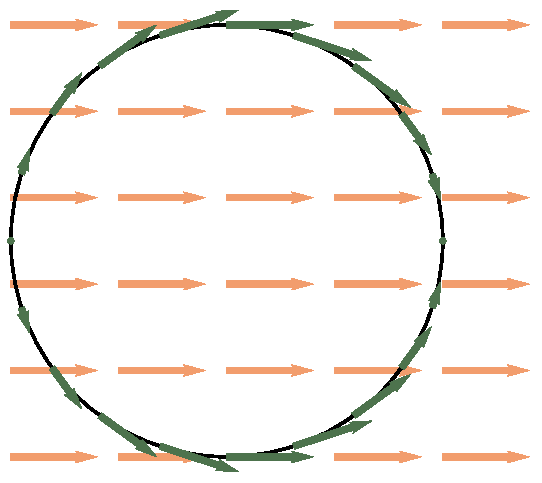
\includegraphics[height=2in]{pullbackdx}
		\caption{The vector field $\frac{\partial}{\partial x}$ (dual to $dx$) on $\R^2$ is shown in orange, and the vector field $-y \frac{\partial}{\partial \theta}$ (dual to $-y\, d\theta = f^\ast dx$) on the circle is shown in green.}
		\alttext{A figure with a white background showing a black circle, a collection of thick orange arrows all of the same length and all pointing to the right, and a collection of thick green arrows of different lengths tangent to various points on the circle.}
		\label{fig:pullback dx}
	\end{figure}
\end{example}

One nice thing about pullbacks is that they commute with the exterior derivative:

\begin{proposition}\label{prop:pullbacks commute with exterior derivative}
	For $f \from M \to N$ smooth and $\omega \in \Omega^k(N)$,
	\[
		d(f^\ast \omega) = f^\ast d\omega.
	\]
\end{proposition}

Before proving this, let's see it in an example:

\begin{example}
	Continuing \cref{ex:1-form in R^3}, recall that $\omega = z \, dy + xy \, dz$ and we computed 
	\[
		d\omega = y\, dx \wedge dz + (x-1) dy \wedge dz.
	\]
	
	Now, consider the map $f \from \R^2 \to \R^3$ given by $f(u,v) = (u^2, u, uv)$. For $p = (u_0, v_0) \in \R^2$ and $w = a \frac{\partial}{\partial u} + b \frac{\partial }{\partial v} \in T_p\R^2$ for $i=1,2$, we can write $w = \alpha_i'(0)$ where $\alpha_i(t) = p + tw = (u_0 , v_0) + t(a,b)$, so 
	\begin{multline*}
		df_p(w) = (f \circ \alpha_i)'(0) = \left. \frac{d}{dt}\right|_{t=0} ((u_0 + ta)^2, u_0 + ta, (u_0 + ta)(v_0 + tb)) \\
		= (2au_0, a, av_0 + bu_0) = 2au_0 \frac{\partial}{\partial x} + a \frac{\partial}{\partial y} + (av_0 + bu_0) \frac{\partial}{\partial z},
	\end{multline*}
	where I'm going back and forth between tuple notation (in $\R^3$ with the standard basis) and local coordinate basis notation (on $T_{f(p)} \R^3$ with the local coordinate basis [which of course is the same as the standard basis]). 
	
	Therefore,
	\begin{multline*}
		(f^\ast \omega)_p(w) = \omega_{f(p)}(df_p(w)) = \left(\vphantom{x^2} u_0v_0 \, dy + u_0^3 \, dz\right)\left(2au_0 \frac{\partial}{\partial x} + a \frac{\partial}{\partial y} + (av_0 + bu_0) \frac{\partial}{\partial z}\right) \\
		= a u_0 v_0(1+u_0^2) + b u_0^4.
	\end{multline*}
	Since this is what the linear functional $(f^\ast \omega)_{(u_0,v_0)}$ does to the tangent vector $w=a \frac{\partial}{\partial u} + b \frac{\partial }{\partial v}$, we see that $(f^\ast \omega)_{(u_0,v_0)} = u_0 v_0(1+u_0^2) du + u_0^4\, dv$ or, now thinking globally,
	\[
		f^\ast \omega = u v(1+u^2) du + u^4 dv.
	\]
	Hence,
	\begin{align*}
		d(f^\ast \omega) & = \left(d\left( u v(1+u^2) \right)\right) \wedge du + \left(d\left(u^4 \right)\right)\wedge dv \\
		 & = \left( \frac{\partial}{\partial u}\left( u v(1+u^2) \right) du + \frac{\partial}{\partial v}\left( u v(1+u^2) \right) dv\right) \wedge du + \left( \frac{\partial}{\partial u}\left(u^4\right) du + \frac{\partial}{\partial v}\left(u^4\right)dv \right) \wedge dv \\
		 & = u(1+u^2) dv \wedge du + 4u^3 du \wedge dv \\
		 & = (3u^3-u) du \wedge dv.
	\end{align*}
	
	On the other hand,
	\begin{align*}
		(f^\ast d\omega)_{p}\left(\frac{\partial}{\partial u}, \frac{\partial}{\partial v}\right) & = (d\omega)_{f(p)} \left(df_{p}\left(\frac{\partial}{\partial u}\right), df_p\left(\frac{\partial}{\partial v}\right)\right) \\
		 & = \left(\vphantom{x^2}u_0 dx \wedge dz + (u_0^2-1) dy \wedge dz\right)\left(2u_0 \frac{\partial}{\partial x} + \frac{\partial}{\partial y} + v_0\frac{\partial}{\partial z}, u_0\frac{\partial}{\partial z}\right) \\
		 & = 3u_0^3 -u_0.
	\end{align*}
	Notice that $(3u_0^3 -u_0)du \wedge dv $ would produce the same output for this (or any other) input, so $(f^\ast d\omega)_{(u_0,v_0)}= (3u_0^3 -u_0)du \wedge dv$. In other words (now thinking globally)
	\[
		f^\ast d\omega = (3u^3-u)du \wedge dv = d(f^\ast \omega),
	\]
	as predicted by \cref{prop:pullbacks commute with exterior derivative}.
\end{example}

\begin{proof}[Proof of \cref{prop:pullbacks commute with exterior derivative}]
	 Let $p \in M$. If $\omega = g\in \Omega^0(N) = C^\infty(N)$, then $f^\ast g = g \circ f$, so $d(f^\ast g ) = d(g \circ f)$. On the other hand, for any $v \in T_pM$, 
	 \[
	 	(f^\ast dg)_pv = dg_{f(p)}(df_p v) = d(g \circ f)_p(v) = d(f^\ast g)_p(v),
	 \]
	 where we used \cref{def:pullback} for the first equality, the Chain Rule for the second, and \cref{ex:pullbacks of functions are compositions} for the third. This completes the proof in the $k=0$ case.
	 
	 Now, suppose $k > 0$ and that $x_1, \dots , x_n$ are local coordinates in a neighborhood of $f(p) \in N$, meaning that $\omega \in \Omega^k(N)$ has the form $\omega_{f(p)} = \sum_I g_I dx_I$ at $f(p)$, so that
	 \[
	 	(d\omega)_{f(p)} = \sum_I dg_I \wedge dx_I.
	 \]
	 But then
	 \[
	 	(f^\ast d\omega)_p = \sum_I (f^\ast dg_I) \wedge (f^\ast dx_I) = \sum_I d(g_I \circ f) \wedge f^\ast dx_{i_1} \wedge \dots \wedge f^\ast dx_{i_k} = \sum_I d(g_I \circ f) \wedge d(x_{i_1} \circ f) \wedge \dots \wedge d(x_{i_k} \circ f),
	 \]
	 where we've repeatedly used both the $k=0$ case and the fact that $f^\ast(\alpha \wedge \beta) = (f^\ast \alpha) \wedge (f^\ast \beta)$ (which follows from HW \#2, Problem 1).
	 
	 On the other hand,
	 \[
	 	(f^\ast\omega)_p = \sum_I (g_I \circ f) f^\ast dx_I = \sum_I (g_I \circ f) f^\ast dx_{i_1} \wedge \dots \wedge f^\ast dx_{i_k} = \sum_I (g_I \circ f) d (x_{i_1} \circ f) \wedge \dots \wedge d(x_{i_k} \circ f),
	 \]
	 so
	 \[
	 	(df^\ast \omega)_p = \sum_I d(g_I \circ f) \wedge d (x_{i_1} \circ f) \wedge \dots \wedge d(x_{i_k} \circ f) = (f^\ast d\omega)_p,
	 \]
	 and we conclude that the proposition is also true for $k>0$.
\end{proof}
% % !TEX root = ../dg.tex

\section{Lie Derivatives and Cartan's Magic Formula}

Recall \cref{def:Lie derivative}, the definition of the Lie derivative for vector fields:
\[
	\mathcal{L}_XY := \lim_{t \to 0} \frac{(d\Phi_{-t})_{\Phi_t(p)}Y(\Phi_t(p))-Y(p)}{t},
\]
where $\Phi_t$ is the local flow for $X \in \mathfrak{X}(M)$. We saw in \cref{prop:Lie bracket = Lie derivative} that the Lie derivative is equal to the Lie bracket $[X,Y]$.

The key idea in this derivative was to compare $Y$ at $\Phi_t(p)$ to $Y$ at $p$, and to do so we needed to move $Y(\Phi_t(p))$ from $T_{\Phi_t(p)}M$ to $T_pM$, which we did with the differential of the \emph{negative} flow $d\Phi_{-t}$.

We can use the same idea to get a Lie derivative for differential forms, though we have to be careful about how we move a form $\omega \in \Omega^k(M)$ at a point $\Phi_t(p)$ to $p$: whereas vector fields push forward, differential forms pull back (as we've just seen in \cref{sec:pullbacks}). So rather than pushing forward with $d\Phi_{-t}$, we will pull back by $\Phi_t^\ast$:

\begin{definition}\label{def:Lie derivative of differential form}
	Let $X \in \mathfrak{X}(M)$ and $\omega \in \Omega^k(M)$. Then the \emph{Lie derivative} of $\omega$ with respect to $X$ is defined (at a point $p \in M$) by
	\[
		\left(\mathcal{L}_X\omega\right)_p := \lim_{t \to 0} \frac{\Phi_t^\ast(\omega_{\Phi_t(p)})-\omega_p}{t} = \left. \frac{d}{dt}\right|_{t=0} \left(\Phi_t^\ast\right)_p(\omega_{\Phi_t(p)}).
	\]
\end{definition}

Even more generally, we can combine pushforwards and pullbacks to get Lie derivatives of arbitrary tensor fields:

\begin{definition}\label{def:Lie derivative of tensor fields}
	Let $X \in \mathfrak{X}(M)$, $a \in \mathcal{T}_r^0(M)$, and $\beta \in \mathcal{T}_0^s(M)$. Then the \emph{Lie derivative} of the $(r,s)$-tensor field $a \otimes \beta$ is defined (at a point $p \in M$) by
	\[
		\left( \mathcal{L}_X a \otimes \beta\right)_p := \left. \frac{d}{dt} \right|_{t=0} \left[ \left(d\Phi_{-t}\right)_{\Phi_t(p)} \left(a _{\Phi_t(p)} \right) \otimes \left(\Phi_t^\ast\right)_p\left(\beta_{\Phi_t(p)}\right)\right].
	\]
	Extending linearly gives the Lie derivative with respect to $X$ for arbitrary elements of $\mathcal{T}_r^s(M)$.
\end{definition}

\begin{lemma}\label{lem:Lie derivative of function}
	For $f \in C^\infty(M) = \Omega^0(M)$ and $X \in \mathfrak{X}(M)$, 
	\[
		\mathcal{L}_Xf = X(f).
	\]
\end{lemma}

\begin{proof}
	By \cref{def:Lie derivative of differential form} (first equality), \cref{ex:pullbacks of functions are compositions} (second), and \cref{def:tangent vector} (third), 
	\[
		\mathcal{L}_Xf = \left. \frac{d}{dt}\right|_{t=0} \Phi_t^\ast(f) = \left. \frac{d}{dt}\right|_{t=0} f \circ \Phi_t = X(f).
	\]
\end{proof}

\begin{example}
	If $M$ is a manifold and $g$ is a Riemannian metric on $M$, a vector field $X \in \mathfrak{X}(M)$ is called a \emph{Killing field}\footnote{Named after Wilhelm Killing.} if $\mathcal{L}_Xg = 0$. Intuitively, this means that the flow generated by $X$ is an isometry: it preserves distances. If you read about general relativity, you will often see references to Killing fields, which encode the symmetries of spacetime.
	
	Let's compute $\mathcal{L}_X g$ for some vector fields $X$ on $S^2$, where $g$ is the standard Riemannian metric induced by the inner product on $\R^3$. If we work in cylindrical coordinates, we have the local coordinate chart $\phi\from (0,2\pi) \to S^2$ given by
	\[
		\phi(\theta, z) = \left(\sqrt{1-z^2}\cos \theta, \sqrt{1-z^2} \sin \theta, z\right).
	\]
	So then our local coordinate basis $\left\{\frac{\partial}{\partial \theta}, \frac{\partial}{\partial z} \right\}$ at a point $p = \phi(\theta_0,z_0)$ looks like
	\[
		\left. \frac{\partial}{\partial \theta}\right|_p = \left. \frac{d}{dt} \right|_{t=0} \phi(\theta_0+t,z_0) = \left(-\sqrt{1-z_0^2}\sin\theta_0, \sqrt{1-z_0^2}\cos \theta_0,z_0\right)
	\]
	and
	\[
		\left. \frac{\partial}{\partial z}\right|_p = \left. \frac{d}{dt} \right|_{t=0} \phi(\theta_0,z_0+t) = \left(-\frac{z_0 \cos \theta_0}{\sqrt{1-z_0^2}},-\frac{z_0 \sin \theta_0}{\sqrt{1-z_0^2}},1\right).
	\]
	See \cref{fig:dtheta and dz 2} (which is the same as \cref{fig:dtheta and dz}).
	\begin{figure}[htbp]
		\centering
			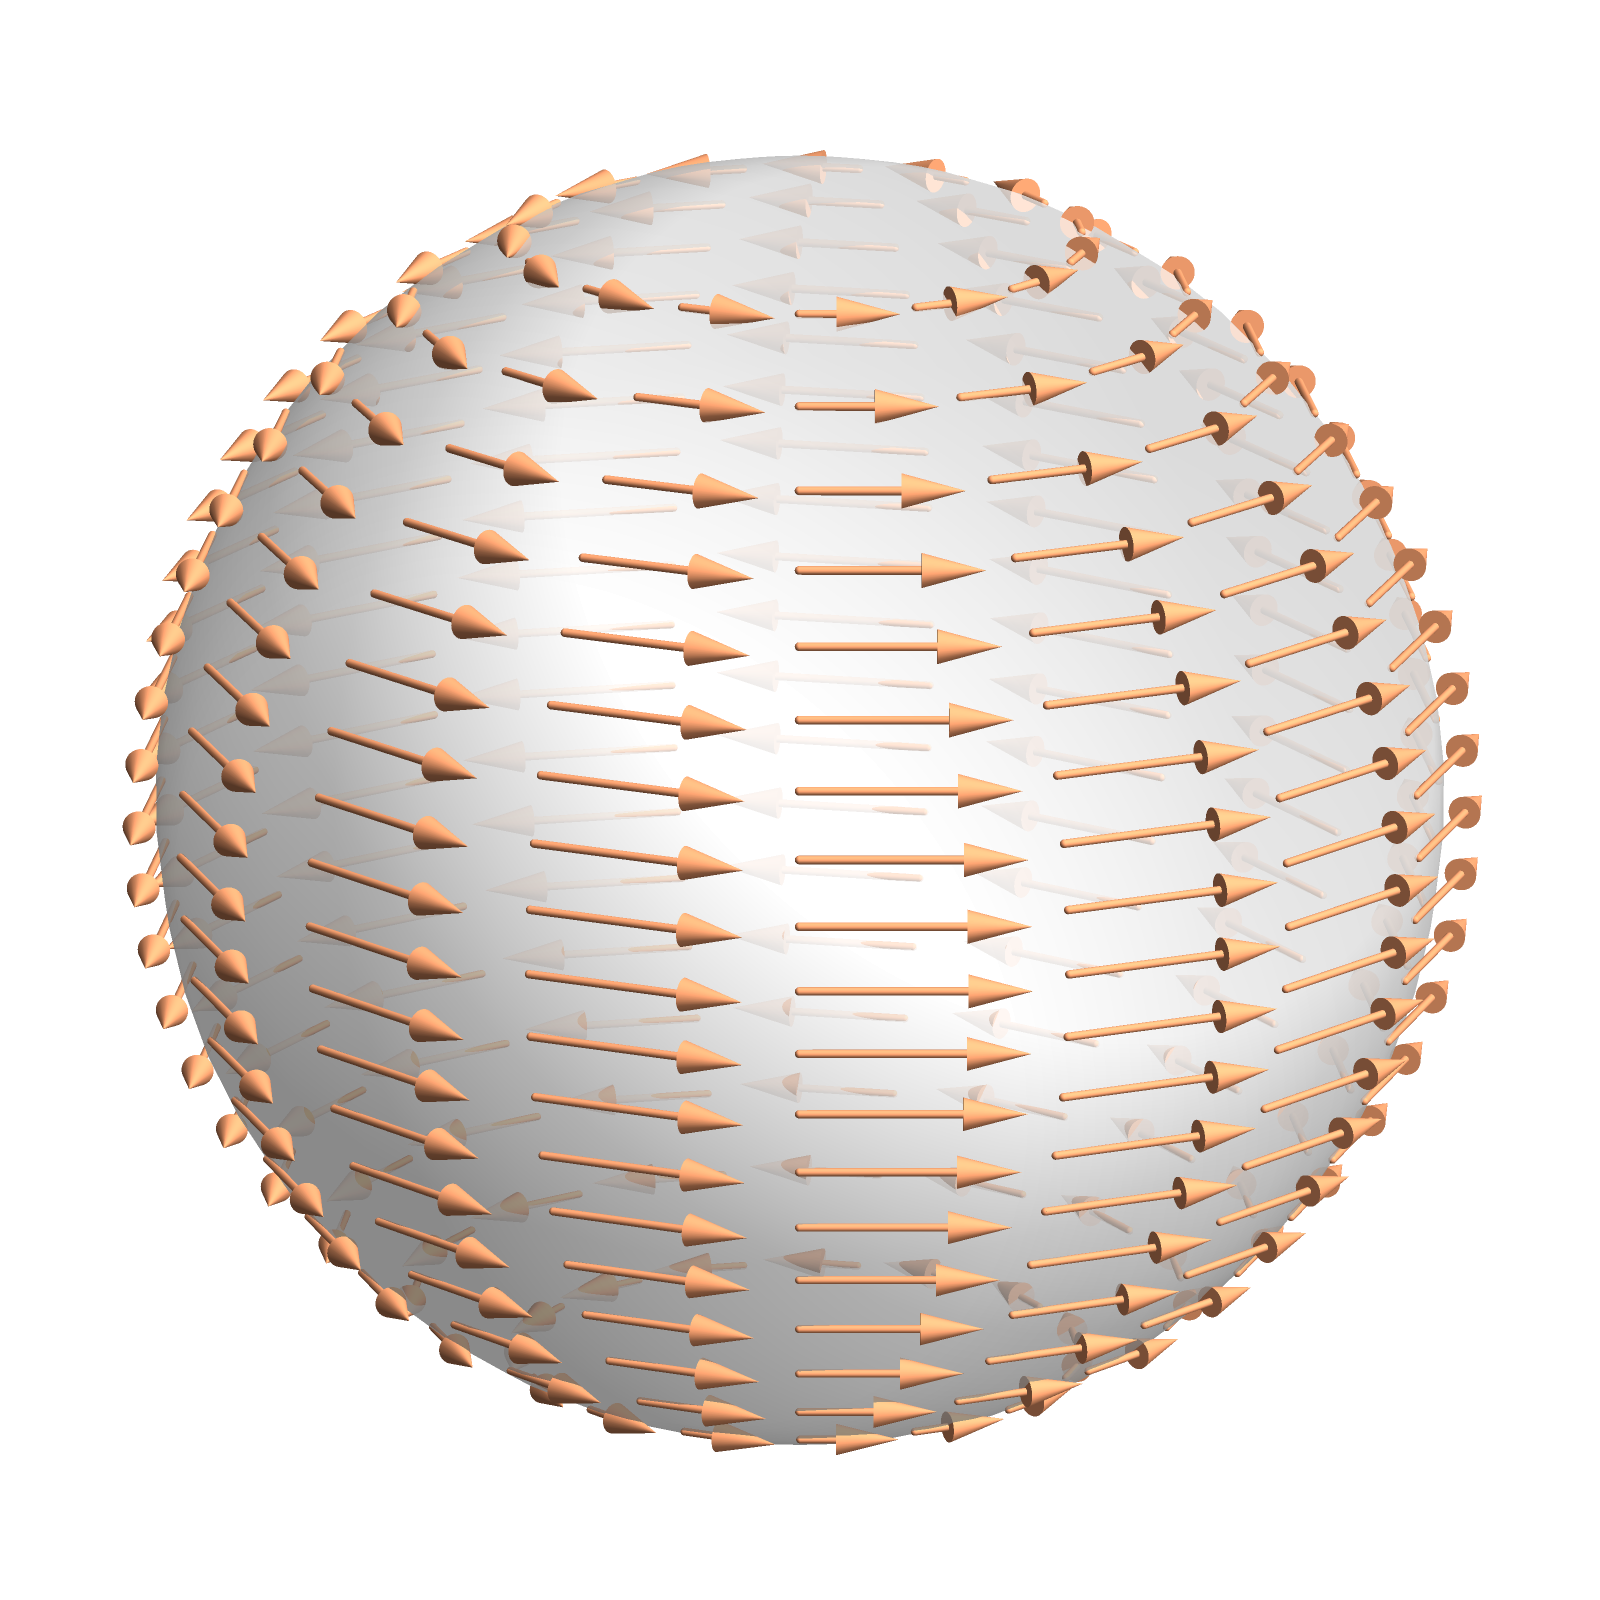
\includegraphics[height=2in]{dtheta} \qquad 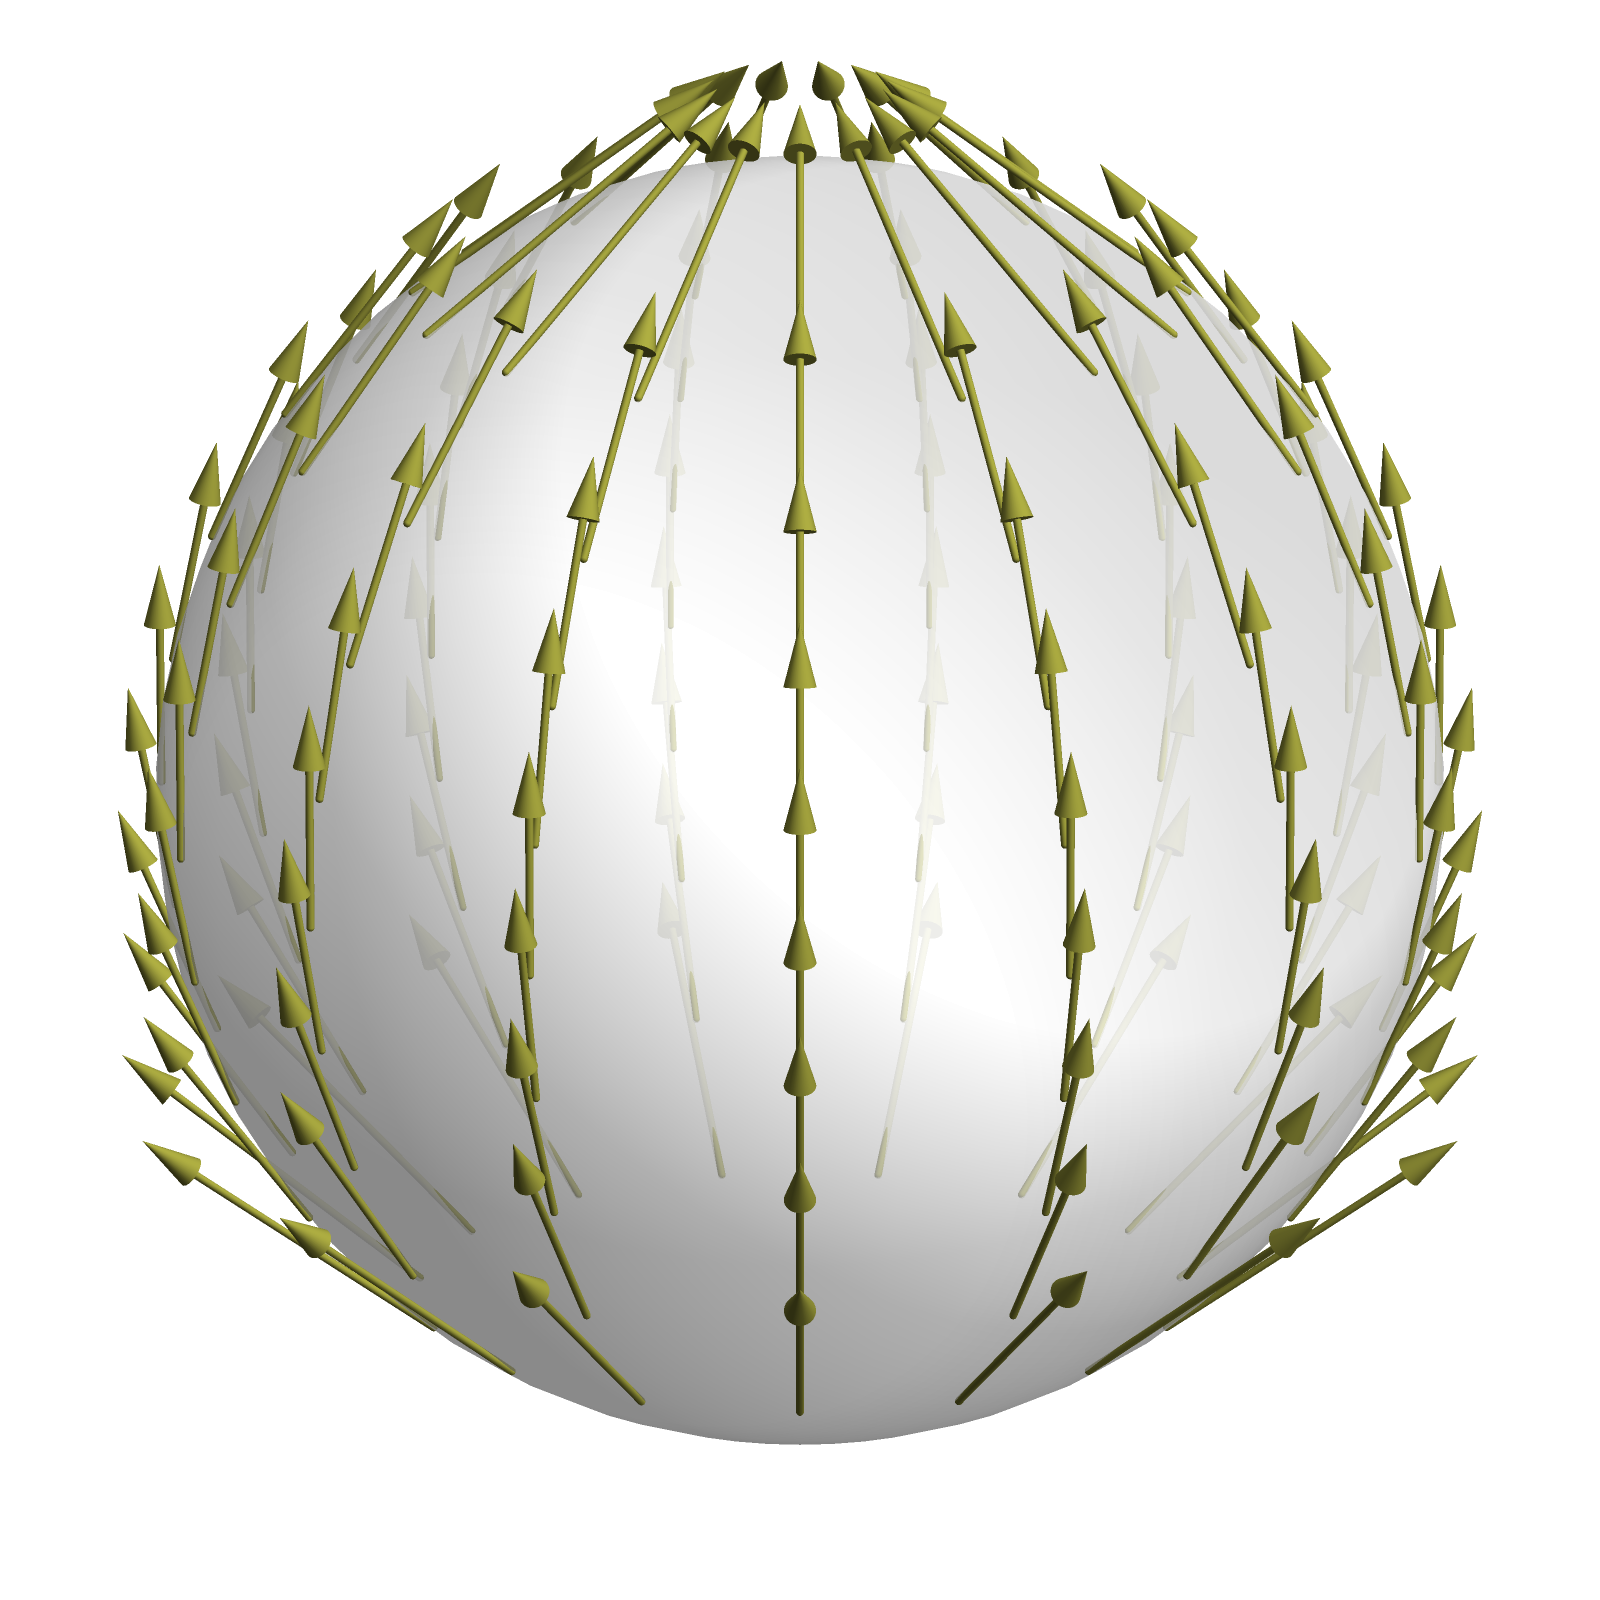
\includegraphics[height=2in]{dz}
		\caption{The vector fields $X = \frac{\partial}{\partial \theta}$ and $Y = \frac{\partial}{\partial z}$ on $S^2$.}
		\alttext{Two computer-generated semi-transparent gray spheres. On the left, a collection of orange arrows or shown on the sphere: the arrows point along circles of latitude: the lengths get shorter as they move away from the equator. On the right, there is a collection of green arrows on the sphere which point towards the north pole. The green arrows get longer as they get further from the equator.}
		\label{fig:dtheta and dz 2}
	\end{figure}
	
	In turn, this implies that the Riemannian metric $g$ is given by
	\begin{align*}
		g_p\left(a \frac{\partial}{\partial \theta} + b \frac{\partial}{\partial z}, c \frac{\partial}{\partial \theta} + d \frac{\partial}{\partial z}\right) & = \left[a\left(-\sqrt{1-z_0^2}\sin\theta_0, \sqrt{1-z_0^2}\cos \theta_0,z_0\right)+ b\left(-\frac{z_0 \cos \theta_0}{\sqrt{1-z_0^2}},-\frac{z_0 \sin \theta_0}{\sqrt{1-z_0^2}},1\right)\right) \\
		& \qquad \cdot \left[c\left(-\sqrt{1-z_0^2}\sin\theta_0, \sqrt{1-z_0^2}\cos \theta_0,z_0\right)+ d\left(-\frac{z_0 \cos \theta_0}{\sqrt{1-z_0^2}},-\frac{z_0 \sin \theta_0}{\sqrt{1-z_0^2}},1\right)\right]  \\
		& = \left(1-z_0^2\right) ac + \frac{1}{1-z_0^2} bd
	\end{align*}
	or, more symbolically,
	\[
		g_{(\theta,z)} = \left(1-z^2\right) d\theta \otimes d\theta + \frac{1}{1-z^2} dz \otimes dz.
	\]
	Notice that this only depends on $z$ and not on $\theta$, so we would expect that flowing by $\frac{\partial}{\partial \theta}$ should preserve this inner product; that is, $\frac{\partial}{\partial \theta}$ should be a Killing field. 
	
	Indeed, the local flow of $\frac{\partial}{\partial \theta}$ is given at a point $p = \phi(\theta_0,z_0)$ by
	\[
		\Phi_t(p) = \phi(\theta_0+t,z) = \left(\sqrt{1-z_0^2}\cos (\theta_0+t), \sqrt{1-z_0^2} \sin (\theta_0+t). z_0\right),
	\]
	Now, writing $\frac{\partial}{\partial \theta} = \alpha'(0)$ where $\alpha(s) = \phi(\theta_0+s,z_0)$, we see that
	\begin{align*}
		(d\Phi_t)_p\left(\left.\frac{\partial}{\partial \theta}\right|_{p}\right) = (d\Phi_t)_p\alpha'(0) & = \left. \frac{d}{ds} \right|_{s=0} (\Phi_t \circ \alpha)(s) \\
		& = \left. \frac{d}{ds} \right|_{s=0} (\Phi_t(\phi(\theta_0+s,z_0)) \\
		& =  \left. \frac{d}{ds} \right|_{s=0} \left(\sqrt{1-z_0^2}\cos (\theta_0+s+t), \sqrt{1-z_0^2} \sin (\theta_0+s+t), z_0\right)  \\
		& = \left(-\sqrt{1-z_0^2}\sin(\theta_0+t),\sqrt{1-z_0^2}\cos(\theta_0+t),0\right) \\
		& = \left. \frac{\partial}{\partial \theta}\right|_{\Phi_t(p)};
	\end{align*}
	i.e., the local flow of $\frac{\partial}{\partial \theta}$ preserves $\frac{\partial}{\partial \theta}$, as you might expect.
	
	On the other hand, $\frac{\partial}{\partial z} = \beta'(0)$ where $\beta(s) = \phi(\theta_0,z_0+s)$, so
	\begin{align*}
		(d\Phi_t)_p\left(\left.\frac{\partial}{\partial z}\right|_{p}\right) = (d\Phi_t)_p\beta'(0) & = \left. \frac{d}{ds} \right|_{s=0} (\Phi_t \circ \beta)(s) \\
		& = \left. \frac{d}{ds} \right|_{s=0} (\Phi_t(\phi(\theta_0,z_0+s)) \\
		& =  \left. \frac{d}{ds} \right|_{s=0} \left(\sqrt{1-(z_0+s)^2}\cos (\theta_0+t), \sqrt{1-(z_0+s)^2} \sin (\theta_0+t), z_0+s\right)  \\
		& = \left(-\frac{z_0 \cos(\theta_0+t)}{\sqrt{1-z_0^2}},-\frac{z_0 \sin(\theta_0+t)}{\sqrt{1-z_0^2}},1\right) \\
		& = \left. \frac{\partial}{\partial z}\right|_{\Phi_t(p)},
	\end{align*}
	so flowing by $\frac{\partial}{\partial \theta}$ also preserves $\frac{\partial}{\partial z}$.

	Therefore, for any $a \left.\frac{\partial}{\partial \theta}\right|_p + b \left.\frac{\partial}{\partial z}\right|_p\in T_pS^2$, we have
	\[
		(d\Phi_t)_p \left(a \left.\frac{\partial}{\partial \theta}\right|_p + b \left.\frac{\partial}{\partial z}\right|_p\right) = a \left.\frac{\partial}{\partial \theta}\right|_{\Phi_t(p)} + b \left.\frac{\partial}{\partial z}\right|_{\Phi_t(p)}.
	\]
	Since $p$ and $\Phi_t(p)$ have the same $z$-coordinate,
	\begin{multline*}
		g_{\Phi_t(p)} \left( a \left.\frac{\partial}{\partial \theta}\right|_{\Phi_t(p)} + b \left.\frac{\partial}{\partial z}\right|_{\Phi_t(p)}, c \left.\frac{\partial}{\partial \theta}\right|_{\Phi_t(p)} + d \left.\frac{\partial}{\partial z}\right|_{\Phi_t(p)}\right) = (1-z_0^2)ac + \frac{1}{1-z_0^2}bd \\
		= g_p\left(a \left.\frac{\partial}{\partial \theta}\right|_p + b \left.\frac{\partial}{\partial z}\right|_p,c \left.\frac{\partial}{\partial \theta}\right|_p + d \left.\frac{\partial}{\partial z}\right|_p\right).
	\end{multline*}
	Hence, for any $u,v \in T_p S^2$
	\[
		(\Phi_t^\ast g_{\Phi_t(p)})(u,v) = g_{\Phi_t(p)}((d\Phi_t)_pu,(d\Phi_t)_pv) = g_p(u,v)
	\]
	is independent of $t$, and we see that
	\[
		(\mathcal{L}_{\frac{\partial}{\partial \theta}} g)_p(u,v) = \left. \frac{d}{dt}\right|_{t=0} (\Phi_t^\ast g_{\Phi_t(p)})(u,v) = 0.
	\]
	Therefore, $\frac{\partial}{\partial \theta}$ is a Killing field on the sphere, which makes sense: the local flow is just rotation around the $z$-axis, which certainly preserves distances.
	
	
	On the other hand, 
	\[
		\Psi_t(p) = \phi(\theta_0,z_0+t) = \left(\sqrt{1-(z_0+t)^2}\cos\theta_0,\sqrt{1-(z_0+t)^2}\sin\theta_0,z_0+t\right)
	\]
	is the local flow of $\frac{\partial}{\partial z}$. So then
	\begin{align*}
		(d\Psi_t)_p\left(\left.\frac{\partial}{\partial \theta}\right|_{p}\right) = (d\Psi_t)_p\alpha'(0) & = \left. \frac{d}{ds} \right|_{s=0} (\Psi_t \circ \alpha)(s) \\
		& = \left. \frac{d}{ds} \right|_{s=0} (\Psi_t(\phi(\theta_0+s,z_0)) \\
		& =  \left. \frac{d}{ds} \right|_{s=0} \left(\sqrt{1-(z_0+t)^2}\cos (\theta_0+s), \sqrt{1-(z_0+t)^2} \sin (\theta_0+s), z_0+t\right)  \\
		& = \left(-\sqrt{1-(z_0+t)^2}\sin\theta_0,\sqrt{1-(z_0+t)^2}\cos\theta_0,0\right) \\
		& = \left. \frac{\partial}{\partial \theta}\right|_{\Psi_t(p)}
	\end{align*}
	and
	\begin{align*}
		(d\Psi_t)_p\left(\left.\frac{\partial}{\partial z}\right|_{p}\right) = (d\Psi_t)_p\beta'(0) & = \left. \frac{d}{ds} \right|_{s=0} (\Psi_t \circ \beta)(s) \\
		& = \left. \frac{d}{ds} \right|_{s=0} (\Psi_t(\phi(\theta_0,z_0+s)) \\
		& =  \left. \frac{d}{ds} \right|_{s=0} \left(\sqrt{1-(z_0+s+t)^2}\cos \theta_0, \sqrt{1-(z_0+s+t)^2} \sin \theta_0, z_0+s+t\right)  \\
		& = \left(-\frac{(z_0+t) \cos\theta_0}{\sqrt{1-(z_0+t)^2}},-\frac{(z_0+t) \sin\theta_0}{\sqrt{1-(z_0+t)^2}},1\right) \\
		& = \left. \frac{\partial}{\partial z}\right|_{\Psi_t(p)},
	\end{align*}
	so flowing by $\frac{\partial}{\partial z}$ also preserves the coordinate vector fields, but the coordinate vector fields do not have constant length on $S^2$. 
	
	We see that 
	\begin{multline*}
		(\Psi_t^\ast g_{\Psi_t(p)})\left(a \left.\frac{\partial}{\partial \theta}\right|_p + b \left.\frac{\partial}{\partial z}\right|_p, c \left.\frac{\partial}{\partial \theta}\right|_p + d \left.\frac{\partial}{\partial z}\right|_p\right) =  g_{\Psi_t(p)}\left(a \left.\frac{\partial}{\partial \theta}\right|_{\Psi_t(p)} + b \left.\frac{\partial}{\partial z}\right|_{\Psi_t(p)}, c \left.\frac{\partial}{\partial \theta}\right|_{\Psi_t(p)} + d \left.\frac{\partial}{\partial z}\right|_{\Psi_t(p)}\right)  \\
		= (1-(z_0+t)^2)ac + \frac{1}{1-(z_0+t)^2}bd,
	\end{multline*}
	and hence
	\begin{multline*}
		(\mathcal{L}_{\frac{\partial}{\partial z}} g)_p\left(\left.\frac{\partial}{\partial \theta}\right|_p,\left.\frac{\partial}{\partial \theta}\right|_p\right) = \left. \frac{d}{dt}\right|_{t=0} (\Psi_t^\ast g_{\Psi_t(p)})\left(\left.\frac{\partial}{\partial \theta}\right|_p,\left.\frac{\partial}{\partial \theta}\right|_p\right) = \left. \frac{d}{dt}\right|_{t=0} \left[(1-(z_0+t)^2)ac + \frac{1}{1-(z_0+t)^2}bd\right] \\
		= -2z_0 ac + \frac{2z_0}{(1-z_0^2)^2}bd;
	\end{multline*}
	that is,
	\[
		\mathcal{L}_{\frac{\partial}{\partial z}} g = -2z\, d\theta \otimes d\theta + \frac{2z}{(1-z^2)^2}dz \otimes dz,
	\]
	which is no longer positive-definite (and hence not a Riemannian metric), but is still a symmetric $(0,2)$-tensor field on $S^2$ which captures how $g$ changes as we flow in the $\frac{\partial}{\partial z}$ direction.
\end{example}

One of the most important formulas in differential geometry is:
\begin{theorem}[Cartan's Magic Formula]\label{thm:cartan}
	If $\omega \in \Omega^k(M)$ and $X \in \mathfrak{X}(M)$, then
	\[
		\mathcal{L}_X \omega = \iota_X d\omega + d \iota_X \omega.
	\]
\end{theorem}
Here $\iota_X$ is the \emph{contraction operator} (or \emph{interior product}) defined as follows: for $\omega \in \Omega^k(M)$ and $X \in \mathfrak{X}(M)$, $\iota_X\omega$ is the $(k-1)$-form defined by
\[
	(\iota_X\omega)_p(v_1, \dots , v_{k-1}) = \omega_p(X(p),v_1, \dots , v_{k-1})
\]
for any $v_1, \dots , v_{k-1} \in T_pM$. This is sometimes also denoted by $X \lrcorner \omega$. This is an antiderivation of degree $-1$.

The reason Cartan's magic formula is so important is that it is one of the most useful tools out there for computing exterior derivatives.

\begin{example}\label{ex:cartan and S^3}
	Remember \cref{sec:S^3 example}, where we computed Lie brackets on $S^3$. As a reminder, we had mutually perpendicular vector fields $X,Y,Z \in \mathfrak{X}(S^3)$ defined by
	\[
		X(p) = pi, \qquad Y(p) = pj, \qquad Z(p) = pk
	\]
	for all $p \in S^3$ thought of as unit quaternions, and showed that
	\[
		[X,Y]=2Z, \qquad [Y,Z] = 2X, \qquad [Z,X] = 2Y.
	\]
	Let $\alpha, \beta, \gamma$ be the dual 1-forms; that is, $\alpha(X) = 1$, $\alpha(Y) = 0 = \alpha(Z)$ and similarly for $\beta$ and $\gamma$. Then, using Cartan's magic formula,
	\[
		d\alpha(Y,Z) = (\iota_Y d\alpha)(Z) = (\mathcal{L}_Y\alpha)(Z) - d(\iota_Y\alpha)(Z) = (\mathcal{L}_Y\alpha)(Z) -d(\alpha(Y))(Z) = (\mathcal{L}_Y\alpha)(Z)
	\]
	since $\alpha(Y) = 0$.
	
	The Lie derivative turns out to be a derivation, so it obeys a Leibniz rule:
	\[
		\mathcal{L}_U(\omega(Y_1, \dots , Y_k)) = (\mathcal{L}_U\omega)(Y_1, \dots , Y_k) + \sum_{j=1}^k \omega(Y_1, \dots , \mathcal{L}_U Y_j, \dots , Y_k).
	\]
	In particular,
	\[
		0 = \mathcal{L}_Y(0) = \mathcal{L}_Y(\alpha(Z)) = (\mathcal{L}_Y \alpha)(Z) + \alpha(\mathcal{L}_YZ) = (\mathcal{L}_Y \alpha)(Z) + \alpha([Y,Z]) = (\mathcal{L}_Y \alpha)(Z) + \alpha(2X) = (\mathcal{L}_Y \alpha)(Z) + 2,
	\]
	so we conclude that
	\[
		d\alpha(Y,Z) = (\mathcal{L}_Y\alpha)(Z) = -2.
	\]
	By analogous calculations, we can show that $d\alpha(X,Y) = 0 = d\alpha(Z,X)$, so we conclude that
	\[
		d\alpha = -2 \beta \wedge \gamma,
	\] 
	and similarly one can show that $d\beta = 2\gamma \wedge \alpha$ and $d\gamma = -2 \alpha \wedge \beta$.
	
	This implies, in particular, that $\alpha \wedge d\alpha = -2 \alpha \wedge \beta \wedge \gamma$ is never zero, so $\alpha$ is an example of what is called a \emph{contact form} on $S^3$.
\end{example}

Notice, in particular, that we never had to work in local coordinates in \cref{ex:cartan and S^3}, which is one of the great virtues of Cartan's magic formula: it is one of the few tools that allows one to compute without using coordinates.

Hopefully this gives you some reason to believe that Cartan's magic formula is useful, so let's try to prove it:

\begin{proof}[Proof of \cref{thm:cartan}]
	If $u \in \Omega^0(M) = C^\infty(M)$, then $\mathcal{L}_Xu = X(u)$ by \cref{lem:Lie derivative of function} and
	\[
		\iota_X du + d\iota_Xu = du(X) + 0 = du(X) = X(u) = \mathcal{L}_Xu ,
	\]
	so the formula holds for 0-forms.
	
	Now consider a 1-form $\omega$ which is the differential of a 0-form: $\omega = du$. If $Y \in \mathfrak{X}(M)$, then, by \cref{def:Lie derivative of differential form},
	\[
		(\mathcal{L}_X\omega)_p(Y) = (\mathcal{L}_xdu)_p(Y) = \left. \frac{d}{dt} \right|_{t=0} \Phi_t^\ast(du_{\Phi_t(p)})(Y) = (\mathcal{L}_xdu)_p(Y) = \left. \frac{d}{dt} \right|_{t=0} du_{\Phi_t(p)}((d\Phi_t)_p(Y))
	\]
	using the definition of pullback (\cref{def:pullback}). In turn, the chain rule tells us that the right hand side is equal to
	\[
		\left. \frac{d}{dt} \right|_{t=0} d(u \circ\Phi_t)_p(Y) = \left. \frac{d}{dt} \right|_{t=0} Y(u \circ\Phi_t)(p)
	\]
	by \cref{lem:vector fields and differentials}. Since $Y$ is independent of $t$, the (1-dimensional) chain rule tell us that this is equal to
	\[
		Y \left( \left. \frac{d(u \circ \Phi_t)}{dt} \right|_{t=0}\right)(p) = Y(X(u))(p).
	\]
	
	So we have shown that $(\mathcal{L}_X\omega)_p(Y) = Y(X(u))(p)$.
	
	On the other hand, $\iota_X d\omega = \iota_X d(du) = 0$ and
	\[
		d(\iota_X\omega)(Y) = d(\iota_X du)(Y) = d(du(X))(Y) = d(X(U))(Y) = Y(X(U)) = (\mathcal{L}_X\omega)_p(Y)
	\]
	by repeatedly using \cref{lem:vector fields and differentials}. Hence, the formula holds for differentials.
	
	Finally, then, if $\omega \in \Omega^k(M)$ and we write $\omega = \sum_I a_I dx_I$ in local coordinates, then
	\begin{equation}\label{eq:cartan in local coords1}
		\mathcal{L}_X\omega = \sum_I \left[ (\mathcal{L}_X a_I)dx_I + a_I \mathcal{L}_X(dx_I)\right].
	\end{equation}
	The $k=0$ argument above implies that 
	\begin{equation}\label{eq:carten in local coords2}
		\mathcal{L}_X a_I = (\iota_X d + d \iota_X)a_I.
	\end{equation} 
	
	On the other hand, again using the fact that the Lie derivative is a derivation, we have
	\begin{multline*}
		\mathcal{L}_X (dx_{i_1} \wedge \dots \wedge dx_{i_k}) = \sum_{j=1}^k dx_{i_1} \wedge \dots \wedge \mathcal{L}_X dx_{i_j}  \wedge \dots \wedge  dx_{i_k} = \sum_{j=1}^k dx_{i_1} \wedge \dots \wedge (\iota_X d + d \iota_X) dx_{i_j}  \wedge \dots \wedge dx_{i_k} \\
		= (\iota_X d + d \iota_X)(dx_{i_1} \wedge \dots \wedge dx_{i_k})
	\end{multline*}
	since each $dx_{i_j}$ is a differential.
	
	Combining this with \eqref{eq:cartan in local coords1} and \eqref{eq:carten in local coords2} implies that 
	\[
		\mathcal{L}_X\omega = \sum_I \left[ ((\iota_X d + d \iota_X) a_I)dx_I + a_I (\iota_X d + d \iota_X)(dx_I)\right] = (\iota_X d + d \iota_X)\sum_I a_I dx_I = (\iota_X d + d \iota_X)\omega,
	\]
	as desired.
\end{proof}
% % !TEX root = ../dg.tex

\section{De Rham Cohomology}
\label{sec:de Rham}

Recall that we have the cochain complex
	\begin{center}
	\begin{tikzcd}
		\Omega^0(M) \arrow[r,"d_0"] & \Omega^1(M) \arrow[r,"d_1"] &  \dots \arrow[r,"d_{n-2}"] & \Omega^{n-1}(M) \arrow[r,"d_{n-1}"] & \Omega^n(M) 
	\end{tikzcd}
	\end{center}
where the subscript $k$ indicates that $d_k$ is the restriction of $d$ to $\Omega^k(M)$.

\begin{definition}\label{def:de Rham cohomology}
	The \emph{$k$th de Rham cohomology group} of $M$ is
	\[
		\hdr^k(M) := \frac{\ker d_k}{\im d_{k-1}}.
	\]
\end{definition}

\begin{example}\label{ex:closed not exact 2}
	We saw in \Cref{ex:closed not exact} that the 1-form $\omega = \frac{x\, dy - y\, dx}{x^2 + y^2} \in \Omega^1(\R^2 -\{0\})$ is \emph{closed} (in the kernel of $d$), but not \emph{exact} (in the image of $d$), so it represents a non-trivial element of $\hdr^1(\R^2 - \{0\})$.
\end{example}

De Rham cohomology is a homotopy invariant of manifolds, meaning that homotopy equivalent manifolds have identical de Rham cohomology groups. 

If $\omega \in \Omega^k(M)$ and $\eta \in \Omega^\ell(M)$ are closed (i.e., $d \omega = 0$ and $d\eta = 0$), meaning that they represent de Rham cohomology classes in $\hdr^k(M)$ and  $\hdr^\ell(M)$, respectively, then
\[
	d(\omega \wedge \eta) = d\omega \wedge \eta + (-1)^k \omega \wedge d\eta = 0 \wedge \eta + (-1)^k \omega \wedge 0 = 0,
\]
so $d(\omega \wedge \eta)$ is also closed, and hence represents a class in $\hdr^{k+\ell}(M)$. This means that
\[
	\hdr^\ast(M) := \bigoplus_k \hdr^k(M)
\]
forms a (graded) ring, the \emph{de Rham cohomology ring}, with the operation induced by $\wedge$.

\begin{theorem}[de Rham theorem]\label{thm:de Rham}
	There exists a vector space isomorphism
	\[
		\hdr^k(M) \to H_k(M;\R)^\ast \cong H^k(M;\R),
	\]
	where $H_k(M;\R)$ and $H^k(M;\R)$ are the singular (or simplicial) homology and cohomology groups.
\end{theorem}

In fact, even more is true: the de Rham cohomology ring is isomorphic to the singular cohomology ring with real coefficients.

In \Cref{ex:closed not exact 2}, $H^1(\R^2 -\{0\};\R) \cong H^1(S^1;\R) \cong \R$, so the 1-form $\omega = \frac{x\, dy - y\, dx}{x^2 + y^2} \in \Omega^1(\R^2 -\{0\})$ is a generator of $\hdr^1(\R^2-\{0\})$.

We won't give all the details of the proof of de Rham's theorem, but the basic idea is that a closed form defines a linear functional on homology classes by integration. More precisely, the mapping $I \from \hdr^k(M) \to H_k(M;\R)^\ast$ is defined as follows: if $[\omega] \in \hdr^k(M)$ is represented by the closed form $\omega \in \Omega^k(M)$, then $I([\omega]) \in H_k(M;\R)^\ast$ is given by
\[
	I([\omega])([C]) := \int_C \omega
\]
for any $[C] \in H_k(M;\R)$ which is represented by the cycle $C \subset M$. It's (hopefully!) clear that $I([\omega])$ is a linear functional (provided the integral here is anything sensible), but probably less obvious that $I$ is well-defined and an isomorphism. Of course, to even make sense of the definition of $I$, we need to talk about integration.

\section{Integration on Manifolds}
\label{sec:integration_on_manifolds}

As suggested in \Cref{sec:informal def of forms}, the point of defining differential forms as alternating, multilinear gadgets is because they transform in the right way. 

\subsection{Digression on Differentials, Pullbacks, and Dual Maps} 
\label{sub:digression_on_differentials_pullbacks_and_dual_maps}

First, a quick refresher on \emph{dual maps} or \emph{algebraic adjoints}:

Given vector spaces $U$ and $V$ and a linear map $h \from U \to V$, there is an associated dual map $h^\ast \from V^\ast \to U^\ast$ defined as follows: if $\alpha \in V^\ast$, then $h^\ast(\alpha)$ is supposed to be an element of $U^\ast$; that is, a linear functional on $U$, meaning that we can specify it by specifying what it does to an arbitrary element $u \in U$:
\[
	h^\ast(\alpha)(u) := \alpha(h(u)).
\]
In other words, $h^\ast \alpha = \alpha \circ h$. It's easy to check that $h^\ast$ is linear since $h$ is.

Moreover, when $U$ and $V$ are finite-dimensional with chosen bases $u_1, \dots , u_m$ for $U$ and $v_1, \dots , v_n$ for $V$, then the matrix for $h^\ast$ with respect to the dual bases $u_1^\ast, \dots , u_m^\ast$ for $U^\ast$ and $v_1^\ast , \dots , v_n^\ast$ for $V^\ast$ is equal to the transpose (or conjugate transpose, for complex vector spaces) of the matrix for $h$ with respect to the given bases for $U$ and $V$. This explains the ``algebraic adjoint'' terminology, since the transpose (or conjugate transpose) is the usual adjoint, at least when the chosen bases are orthonormal. (And I claim it is occasionally useful to think about transpose in these terms, even though in applications we often think about the transpose as just a map $V \to U$.)

Now, consider a smooth map $g \from M \to N$ and let $p \in M$. Then the differential $dg_p \from T_pM \to T_{g(p)}N$ must have an associated dual map $(dg_p)^\ast \from (T_{g(p)}N)^\ast \to (T_pM)^\ast$.

First of all, notice that $\left(T_{g(p)}N\right)^\ast = \ext{1}\left(\left(T_{g(p)}N\right)^\ast\right)$ and $\left(T_pM\right)^\ast = \ext{1}\left(\left(T_pM\right)^\ast\right)$, so the pullback (at $p$)
\[
	g_p^\ast \from \ext{1}\left(\left(T_{g(p)}N\right)^\ast\right)\to \ext{1}\left(\left(T_pM\right)^\ast\right)
\]
has the same domain and range as $(dg_p)^\ast$.

Moreover, by definition of the dual map, for a linear functional $\alpha \in (T_{g(p)}N)^\ast$ and a tangent vector $v \in T_pM$,
\[
	(dg_p)^\ast (\alpha)(v) = \alpha(dg_p(v)).
\]
But this is exactly how we defined the pullback, where we now think of $\alpha = \omega_{g(p)}$, the value of the 1-form $\omega$ at $g(p)$.

In other words, $g^\ast$ as defined in \Cref{sec:pullbacks} is the same as the dual map $(dg)^\ast$ associated to the differential $dg$.

\subsection{How Differential Forms Transform} 
\label{sub:how_differential_forms_transform}

The goal is to see that transformations of differential forms under changes of coordinates are just like transformations of integrands under changes of coordinates.

As in \Cref{sec:informal def of forms}, let $g \from B \to A$ be a diffeomorphism of open subsets of $\R^n$ and let $f \from A \to \R$ be a smooth function. Define
\[
	\omega = f dx_1 \wedge \dots \wedge dx_n \in \Omega^n(A),
\]
which pulls back to
\[
	g^\ast \omega = (f \circ g) g^\ast (dx_1) \wedge \dots \wedge g^\ast(dx_n) = (f \circ g) (dg)^\ast (dx_1) \wedge \dots \wedge (dg)^\ast (dx_n),
\]
where here $(dg)^\ast$ means the dual of the differential $dg$. By Homework 2, Problem 1(c), the above is equal to 
\[
	(f \circ g) (\det (dg)^\ast) dy_1 \wedge \dots \wedge dy_n,
\]
where we recall that $y_1, \dots , y_n$ were just the names of the coordinates on $B$. Since determinants are invariant under taking transposes, $\det(dg)^\ast = \det dg = \det Jg$, so this parallels the usual vector calculus change of variables formula, at least when $f$ is smooth.

In other words, differential forms transform in the right way to serve as integrands.

\begin{example}
	Let $M = (0, +\infty) \times (-\pi, \pi)$, $N = \R^2$, and the map $g\from M \to N$ given by
	\[
		g(r, \theta) := (r \cos \theta, r \sin \theta).
	\]
	In other words, this is the change of variables map between polar coordinates $(r, \theta)$ and Cartesian coordinates $(x,y)$ on the plane.
	
	Now, consider the standard area form $\omega = dx \wedge dy$ on $N$ and we want to work out $g^\ast \omega$ from the definition. 
	
	By definition of the differential (\Cref{def:differential}), we have that, for $p = (\theta_0, r_0) \in M$, 
	\begin{multline*}
		dg_p\left(\frac{\partial}{\partial \theta} \right) = \left. \frac{d}{dt} \right|_{t=0} g(\theta_0+t,r_0) = \left. \frac{d}{dt} \right|_{t=0} r_0(\cos(\theta_0+t),\sin(\theta_0+t)) \\
		= r_0(-\sin\theta_0,\cos\theta_0) = r_0\left(-\sin\theta_0 \frac{\partial}{\partial x} + \cos \theta_0 \frac{\partial}{\partial y}\right)
	\end{multline*}
	where I move back and forth between tuple representations and local coordinate basis representations. Similarly,
	\begin{multline*}
		dg_p\left(\frac{\partial}{\partial r} \right) = \left. \frac{d}{dt} \right|_{t=0} g(\theta_0,r_0+t) = \left. \frac{d}{dt} \right|_{t=0} (r_0+t)(\cos\theta_0,\sin\theta_0) \\
		= (\cos\theta_0,\sin\theta_0) = \cos\theta_0 \frac{\partial}{\partial x} + \sin \theta_0 \frac{\partial}{\partial y}.
	\end{multline*}
	
	Therefore,
	\begin{align*}
		(g^\ast \omega)_p\left(a \frac{\partial}{\partial \theta} + b \frac{\partial}{\partial r}, c \frac{\partial}{\partial \theta} + d \frac{\partial}{\partial r}\right) & = \omega_{g(p)} \left(dg_p\left(a \frac{\partial}{\partial \theta} + b \frac{\partial}{\partial r}\right), dg_p\left(c \frac{\partial}{\partial \theta} + d \frac{\partial}{\partial r}\right)\right) \\
		& = dx \wedge dy \left((b \cos\theta_0 - a r_0\sin\theta_0) \frac{\partial}{\partial x} + (b\sin \theta_0 +ar_0\cos \theta_0) \frac{\partial}{\partial y}, \right. \\
		& \qquad \qquad \qquad \left. (d \cos\theta_0 - c r_0\sin\theta_0) \frac{\partial}{\partial x} + (d\sin \theta_0 +cr_0\cos \theta_0) \frac{\partial}{\partial y}\right) \\
		& = (b \cos\theta_0 - a r_0\sin\theta_0)(d\sin \theta_0 +cr_0\cos \theta_0) \\
		& \qquad \qquad - (b\sin \theta_0 +ar_0\cos \theta_0)(d \cos\theta_0 - c r_0\sin\theta_0) \\
		& = r(bc-ad).
	\end{align*}
	On the other hand,
	\[
		dr \wedge d\theta \left(a \frac{\partial}{\partial \theta} + b \frac{\partial}{\partial r}, c \frac{\partial}{\partial \theta} + d \frac{\partial}{\partial r}\right) = bc-ad,
	\]
	so we can conclude that $g^\ast \omega = r\, dr \wedge d\theta$.
	
	Since the composition of the constant function 1 (on $N$) with $g$ is just the constant function 1 (on $M$), the above discussion implies that
	\[
		g^\ast \omega = g^\ast(dx \wedge dy) = (\det Jg) dr \wedge d\theta,
	\]
	where $\det Jg$ is the Jacobian determinant
	\[
		\begin{vmatrix} \frac{\partial g_1}{\partial r} & \frac{\partial g_1}{\partial \theta} \\ \frac{\partial g_2}{\partial r} & \frac{\partial g_2}{\partial \theta} \end{vmatrix} = \begin{vmatrix}\cos\theta & -r \sin \theta  \\ \sin \theta  & r \cos \theta\end{vmatrix} = r \cos^2\theta+r\sin^2\theta  = r.
	\]
	So the above discussion of how differential forms transform matches up to the standard vector calculus fact that the Cartesian area element $dx\, dy$ transforms to the polar area element $r\, dr \, d\theta$.
\end{example}

\subsection{Definition of the Integral}
\label{sub:definition_of_the_integral}

First, we define integration of forms on open sets in $\R^n$: if $A \subset \R^n$ is open, then any $\omega \in \Omega^n(A)$ can be written as
\[
	\omega = f\, dx_1 \wedge \dots \wedge dx_n,
\]
where $f$ is a smooth function on $A$. Define
\[
	\int_A \omega = \int_A f \, dx_1 \cdots dx_n,
\]
where the integral on the right is just the usual Riemann integral of the (smooth) function $f$ over $A$.

By the previous discussion, if $g \from B \to A$ is an orientation-preserving diffeomorphism, then $\det Jg > 0$, so
\begin{multline*}
	\int_A \omega = \int_A f \, dx_1 \cdots dx_n = \int_B(f \circ g) |\det Jg| \, dy_1 \cdots dy_n = \int_B (f \circ g) (\det Jg) \, dy_1 \cdots dy_n \\
	 = \int_B(f \circ g) (\det Jg) dy_1 \wedge \dots \wedge dy_n = \int_B g^\ast \omega.
\end{multline*}
In other words, our definition is actually coordinate-independent, as you would hope.

If $g$ is orientation-reversing, then we get
\[
	\int_A \omega = -\int_B g^\ast \omega.
\]

Since we have no standard coordinates on an arbitrary manifold, these transformations are essential to defining integrals on manifolds.

Suppose next that we have an $n$-dimensional manifold $M$ and the support of $\omega \in \Omega^n(M)$ is contained in a single coordinate chart $(U,\phi)$ so that $\phi \from U \to \phi(U)$ is orientation-preserving. Then $\phi^\ast \omega \in \Omega^n(U)$, which we know how to integrate, so define
\[
	\int_M\omega = \int_U \phi^\ast \omega.
\]

\begin{proposition}\label{prop:local integral well-defined}
	The above is well-defined.
\end{proposition}

\begin{proof}
	We need to check that, if the support of $\omega$ is also contained in some other coordinate chart $(V, \psi)$ so that $\psi \from V \to \psi(V)$ is orientation-preserving, then we get the same answer whether we compute $\int_M \omega = \int_U \phi^\ast \omega$ or $\int_M \omega = \int_V \psi^\ast \omega$.
	
	We can move between $U$ and $V$ by way of the map $\psi^{-1} \circ \phi \from U \to V$, which is orientation-preserving, so
	\[
		\int_V \psi^\ast \omega = \int_U(\psi^{-1} \circ \phi)^\ast \psi^\ast \omega = \int_U \phi^\ast (\psi^{-1})^\ast \psi^\ast \omega = \int_U \phi^\ast (\psi \circ \psi^{-1})\ast \omega = \int_U \phi^\ast \omega ,
	\]
	where I'm using the previously unstated fact that, for maps $f \from A \to B$ and $g \from B \to C$, $(g \circ f)^\ast = f^\ast g^\ast$, which follows from the chain rule.
\end{proof}

So we've now succeeded in defining the integral of a form contained entirely in a single local coordinate chart. But what about arbitrary forms?

First of all, to avoid worrying about convergence issues, let's restrict to \emph{compactly supported} forms: that is, those forms whose support (the set of points on which they are non-vanishing) is contained in some compact subset of $M$. Of course, if $M$ is itself compact, this is no restriction at all.

So now suppose we have a compactly supported form $\omega \in \Omega^n(M)$. To define $\int_M \omega$, we will use a partition of unity argument.

\begin{definition}\label{def:partition of unity}
	Let $T$ be a topological space and let $\{W_\alpha\}_{\alpha \in \mathcal{I}}$ be an open cover of $T$, where $\mathcal{I}$ us some indexing set. A \emph{partition of unity} subordinate to $\{W_\alpha\}_{\alpha \in \mathcal{I}}$ is a collection $\{\rho_\alpha\}_{\alpha \in \mathcal{I}}$ of continuous functions $\rho_\alpha \from T \to [0,1]$ so that $\operatorname{supp}(\rho_\alpha) \subset W_\alpha$ (i.e., $\rho_\alpha(x) = 0$ for all $x \notin W_\alpha$) and, for all $x \in T$,
	\begin{itemize}
		\item there exists a neighborhood of $x$ on which all but finitely many of the $\rho_\alpha$ are identically zero and
		\item $\sum_{\alpha \in \mathcal{I}} \rho_\alpha(x) = 1$ (note that the previous condition ensures this sum is finite and hence converges).
	\end{itemize}
\end{definition}

These always exist in reasonable topological spaces:

\begin{theorem}\label{thm:existence of partitions of unity}
	Every open cover on a paracompact Hausdorff space has a subordinate partition of unity.
\end{theorem}

Since manifolds are second countable and Hausdorff, they are paracompact, so this implies (after modifying the proof to make the $\rho_\alpha$ smooth):

\begin{corollary}\label{cor:existence of partitions of unity on manifolds}
	Every manifold has a partition of unity subordinate to its coordinate atlas so that the functions are smooth.
\end{corollary}

Now, finally, we can define integration of compactly-supported forms on manifolds:

\begin{definition}\label{def:integration}
	Let $M$ be an $n$-dimensional manifold and let $\omega \in \Omega^n(M)$ be compactly supported. Let $\{\rho_\alpha\}$ be a partition of unity subordinate to the (maximal) atlas $\{(U_\alpha, \phi_\alpha)\}$ on $M$ and define
	\[
		\int_M \omega = \sum_{\alpha} \int_M \rho_\alpha \omega.
	\]
\end{definition}

\begin{remark}
	\begin{enumerate}
		\item $\rho_\alpha \omega$ is only non-vanishing inside the support of $\rho_\alpha$, which is contained in some coordinate neighborhood $\phi_\alpha(U_\alpha)$, so the integrals inside the sum are well-defined.
		\item The local finiteness of the partition of unity guarantees only finitely many terms are nonzero on the compact support of $\omega$, so the sum converges.
		\item If $\omega$ is already contained in some coordinate chart $(\phi, U)$, then this definition agrees with the previous one: since $\sum_\alpha \rho_\alpha(p) = 1$ for each $p \in M$, we have that $\sum_\alpha \rho_\alpha \omega = \omega$, so using the previous definition
		\[
			\int_M \omega = \int_U \phi^\ast \omega = \int_U \phi^\ast(\sum_\alpha \rho_\alpha \omega) = \sum_\alpha \int_U \phi^\ast(\rho_\alpha \omega) = \sum_\alpha \int_M \rho_\alpha \omega
		\]
		by linearity of pullback and of integration on $\R^n$.
		\item If $\{\sigma_\alpha\}$ were a different subordinate partition of unity, then the previous observation implies that, or each $\alpha$,
		\[
			\int_M \rho_\alpha \omega = \sum_\beta \int_M \sigma_\beta \rho_\alpha \omega
		\]
		and similarly for each $\beta$
		\[
			\int_M \sigma_\beta \omega = \sum_\alpha \int_M \rho_\alpha \sigma_\beta \omega,
		\]
		so
		\[
			\sum_\alpha \int_M \rho_\alpha \omega = \sum_\alpha \sum_\beta \int_M \sigma_\beta \rho_\alpha \omega = \sum_\beta \sum_\alpha \int_M \rho_\alpha \sigma_\beta \omega = \sum_\beta \int_M \sigma_\beta \omega,
		\]
		which means we get the same value for $\int_M \omega$ no matter which partition of unity we use.
		\item Integration is a linear operator: for $a \in \R$ and $\omega, \eta \in \Omega^n(M)$, $\int_M (\omega + a \eta) = \int_M \omega + a \int_M \eta$.
		\item If $\omega \in \Omega^n(M)$ and $g \from N \to M$ is an orientation-preserving diffeomorphism, then
		\[
			\int_M \omega = \int_N g^\ast \omega.
		\]
	\end{enumerate}
\end{remark}

\begin{example}\label{ex:integrating along a curve}
	Let $\gamma \from [a,b] \to M$ be a smooth curve with $\gamma(a) = p$ and $\gamma(b) = q$. Assume $f \in C^\infty(M)$ and $\omega = df \in \Omega^1(M)$. Then I claim that
	\[
		\int_{[a,b]} \gamma^\ast \omega = f(q) - f(p).
	\]
	This is just a computation:
	\begin{multline*}
		\int_{[a,b]} \gamma^\ast \omega = \int_{[a,b]}\gamma^\ast(df) = \int_{[a,b]} d (\gamma^\ast f) = \int_{[a,b]} d(f \circ \gamma) = \int_{[a,b]}(f \circ \gamma)'(t)dt \\
		= (f \circ \gamma)(b) - (f\circ \gamma)(a) = f(q)-f(p)
	\end{multline*}
	where the second equality follows from \Cref{prop:pullbacks commute with exterior derivative}, the third from \Cref{ex:pullbacks of functions are compositions}, and the fifth from the fundamental theorem of calculus.
\end{example}

\begin{example}\label{ex:line integral}
	Suppose $\gamma \from S^1 \to M$ is smooth and $\omega \in \Omega^1(M)$. Then we define the \emph{line integral} of $\omega$ around $\gamma$ to be
	\[
		\oint_\gamma \omega := \int_{S^1} \gamma^\ast \omega.
	\]
	Now suppose $M = \R^n$, so that $\omega = a_1 \, dx_1 + \dots + a_n \, dx_n$. Letting $\left\{\frac{\partial}{\partial \theta}\right\}$ be the local coordinate basis for the tangent space $T_t S^1$ at a point $t \in S^1$ and writing $\gamma(t) = (\gamma_1(t), \dots , \gamma_n(t))$, we can compute
	\[
		(\gamma^\ast dx_i)_t \left(b \frac{\partial}{\partial \theta} \right) = (dx_i)_{\gamma(t)} \left(d\gamma_t\left(b \frac{\partial}{\partial \theta}\right)\right) = b (dx_i)_{\gamma(t)} \left(d\gamma_t\left(\frac{\partial}{\partial \theta}\right)\right) = b (dx_i)_{\gamma(t)} \left(\frac{\partial}{\partial \theta}(\gamma)(t)\right) 
	\]
	using \Cref{lem:vector fields and differentials}. But then
	\[
		\frac{\partial}{\partial \theta}(\gamma)(t) = \gamma_1'(t) \frac{\partial}{\partial x_1} + \dots + \gamma_n'(t) \frac{\partial}{\partial x_n},
	\]
	so we see that 
	\[
		(\gamma^\ast dx_i)_t \left(b \frac{\partial}{\partial \theta} \right) = b \gamma_i'(t)
	\]
	or, in other words, $(\gamma^\ast dx_i)_t = \gamma_i'(\theta)d\theta$. Therefore,
	\[
		(\gamma^\ast \omega)_t = (\gamma^\ast a_1)_t (\gamma^\ast dx_1)_t + \dots + (\gamma^\ast a_n)_t (\gamma^\ast dx_n)_t = \left[a_1(\gamma(t)) \gamma_1'(t) + \dots + a_n(\gamma(t))\gamma_n'(t)\right] d\theta.
	\]
	Notice that the coefficient is just $A(\gamma(t))\cdot \gamma'(t)$, where the vector field $A = (a_1, \dots , a_n)$ is dual to $\omega$. Of course, this is the sort of expression you usually see in the Multivariable Calculus definition of a line integral.
\end{example}

Putting \Cref{ex:integrating along a curve,ex:line integral} together, notice that if $\omega = df \in \Omega^1(M)$, then $\oint_\gamma \omega = 0$ for all closed curves $\gamma$ in $M$.

\begin{proposition}\label{prop:integrate to 0 => exact}
	The converse is true. That is, any $\omega \in \Omega^1(M)$ with the property that $\oint_\gamma \omega = 0$ for all closed curves $\gamma$ in $M$ is exact.
\end{proposition}

\begin{exercise}
	Prove this.
\end{exercise}




\bibliography{dg}

\end{document}
